\documentclass[10pt,a4paper]{article}
%DIF LATEXDIFF DIFFERENCE FILE
%DIF DEL old.tex   Sat Nov  7 15:21:29 2026
%DIF ADD new.tex   Sat Nov  7 15:21:29 2026
\usepackage[margin=23mm]{geometry}
\usepackage{nature_reading}
\usepackage{longtable}
% Generated from pinned audit evidence.
\newcommand{\TrainSeconds}{361.6}
\newcommand{\TrainMemory}{0.543}
\newcommand{\FirstIdentity}{1.17}
\newcommand{\FirstShuffled}{1.17}
\newcommand{\FirstZero}{0.00}
\newcommand{\BlockIdentity}{0.586}
\newcommand{\BlockGain}{0.098}
\newcommand{\BlockLow}{0.000}
\newcommand{\BlockHigh}{0.307}
\newcommand{\BlockFone}{0.320}
\newcommand{\RunDecision}{reject}

% Generated from the pinned V54 audit; no fitted presentation values.
\newcommand{\DensitySeconds}{207.8}
\newcommand{\DensityMemory}{0.400}
\newcommand{\DensityNll}{15.219}
\newcommand{\DensityShuffledNll}{15.254}
\newcommand{\DensityAdvantage}{0.0355}
\newcommand{\DensityLow}{-0.1014}
\newcommand{\DensityHigh}{0.1693}
\newcommand{\DensityIdentity}{1.562}
\newcommand{\DensityFone}{0.350}
\newcommand{\DensityCopyFone}{0.99949}
\newcommand{\DensityDecision}{reject}

% Generated from the locked V55 matched audit.
\newcommand{\JointNll}{7.026}
\newcommand{\ControlNll}{7.579}
\newcommand{\JointNllGain}{0.553}
\newcommand{\JointNllLow}{0.450}
\newcommand{\JointNllHigh}{0.665}
\newcommand{\JointTime}{342.4}
\newcommand{\ControlTime}{218.0}
\newcommand{\JointMemory}{0.648}
\newcommand{\ControlMemory}{0.400}
\newcommand{\JointSampleFone}{0.362}
\newcommand{\JointPrefixGain}{0.185}
\newcommand{\JointDecision}{reject}

% Generated from unchanged V56 report.
\newcommand{\BeamAccuracy}{11.621}
\newcommand{\BeamShuffled}{9.863}
\newcommand{\GreedyAccuracy}{8.252}
\newcommand{\BeamGain}{3.369}
\newcommand{\BeamGainLow}{2.351}
\newcommand{\BeamGainHigh}{4.412}
\newcommand{\BeamHistoryGain}{1.758}
\newcommand{\BeamHistoryLow}{0.966}
\newcommand{\BeamHistoryHigh}{2.552}
\newcommand{\BeamRepeat}{25.446}
\newcommand{\TargetRepeat}{0.112}
\newcommand{\BeamSeconds}{269.3}
\newcommand{\BeamMemory}{0.154}
\newcommand{\BeamDecision}{reject\_decoder}

% Generated from the completed V57 audit.
\newcommand{\QaExact}{3.906}
\newcommand{\QaFone}{15.718}
\newcommand{\QaBlankExact}{0.391}
\newcommand{\QaBlankFone}{5.553}
\newcommand{\QaControlExact}{0.000}
\newcommand{\QaControlFone}{6.582}
\newcommand{\QaQuestionGain}{10.165}
\newcommand{\QaQuestionLow}{7.043}
\newcommand{\QaQuestionHigh}{13.371}
\newcommand{\QaPairExact}{0.254}
\newcommand{\QaMotor}{100.000}
\newcommand{\QaSeconds}{278.572}
\newcommand{\QaMemory}{1.053}
\newcommand{\QaControlSeconds}{269.126}
\newcommand{\QaControlMemory}{1.049}
\newcommand{\QaDecision}{reject\_reading\_model}

% Generated from the fixed autonomous verification receipt.
\newcommand{\CodecLanguageFOne}{32.671}
\newcommand{\CodecLanguageBlankFOne}{19.508}
\newcommand{\CodecLanguageQuestionGain}{13.163}
\newcommand{\CodecLanguageCILow}{10.933}
\newcommand{\CodecLanguageCIHigh}{15.730}
%DIF PREAMBLE EXTENSION ADDED BY LATEXDIFF
%DIF CFONT PREAMBLE %DIF PREAMBLE
\RequirePackage{color}\definecolor{RED}{rgb}{1,0,0}\definecolor{BLUE}{rgb}{0,0,1} %DIF PREAMBLE
\DeclareOldFontCommand{\sf}{\normalfont\sffamily}{\mathsf} %DIF PREAMBLE
\providecommand{\DIFadd}[1]{{\protect\color{blue} \sf #1}} %DIF PREAMBLE
\providecommand{\DIFdel}[1]{{\protect\color{red} \scriptsize #1}} %DIF PREAMBLE
%DIF SAFE PREAMBLE %DIF PREAMBLE
\providecommand{\DIFaddbegin}{} %DIF PREAMBLE
\providecommand{\DIFaddend}{} %DIF PREAMBLE
\providecommand{\DIFdelbegin}{} %DIF PREAMBLE
\providecommand{\DIFdelend}{} %DIF PREAMBLE
\providecommand{\DIFmodbegin}{} %DIF PREAMBLE
\providecommand{\DIFmodend}{} %DIF PREAMBLE
%DIF IDENTICAL PREAMBLE %DIF PREAMBLE
\providecommand{\DIFaddFL}[1]{\DIFadd{#1}} %DIF PREAMBLE
\providecommand{\DIFdelFL}[1]{\DIFdel{#1}} %DIF PREAMBLE
\providecommand{\DIFaddbeginFL}{\DIFaddbegin} %DIF PREAMBLE
\providecommand{\DIFaddendFL}{\DIFaddend} %DIF PREAMBLE
\providecommand{\DIFdelbeginFL}{\DIFdelbegin} %DIF PREAMBLE
\providecommand{\DIFdelendFL}{\DIFdelend} %DIF PREAMBLE
%DIF COLORLISTINGS PREAMBLE %DIF PREAMBLE
\RequirePackage{listings} %DIF PREAMBLE
\RequirePackage{color} %DIF PREAMBLE
\lstdefinelanguage{DIFcode}{ %DIF PREAMBLE
%DIF DIFCODE_CFONT %DIF PREAMBLE
  moredelim=[il][\color{red}\scriptsize]{\%DIF\ <\ }, %DIF PREAMBLE
  moredelim=[il][\color{blue}\sffamily]{\%DIF\ >\ } %DIF PREAMBLE
} %DIF PREAMBLE
\lstdefinestyle{DIFverbatimstyle}{ %DIF PREAMBLE
	language=DIFcode, %DIF PREAMBLE
	basicstyle=\ttfamily, %DIF PREAMBLE
	columns=fullflexible, %DIF PREAMBLE
	keepspaces=true %DIF PREAMBLE
} %DIF PREAMBLE
\lstnewenvironment{DIFverbatim}[1][]{\lstset{style=DIFverbatimstyle}}{} %DIF PREAMBLE
\lstnewenvironment{DIFverbatim*}[1][]{\lstset{style=DIFverbatimstyle,showspaces=true}}{} %DIF PREAMBLE
\lstset{extendedchars=\true,inputencoding=utf8}

%DIF END PREAMBLE EXTENSION ADDED BY LATEXDIFF

\begin{document}
\noindent{\color{blue}\footnotesize Change-marked copy: additions relative to the V68 conditional-writing baseline are blue.}\par\medskip

\renewcommand{\thefigure}{S\arabic{figure}}
{\sffamily\bfseries\Large Supplementary Information\par}
\medskip\noindent\textbf{Learning conditional language in continuous image space}\par
\medskip\noindent Imagized Language Model Project

\section*{Supplementary Note 1: experimental question and scope}
The target is an independent visual language model whose runtime consumes
writing images and generates writing images. Encoded text and local language
models may prepare data offline. They cannot supply the answer during model
inference. The present experiment isolates canonical Chinese continuation as
one prerequisite. It does not cover the complete instruction-following or
historical-script objective.

The repository retains the earlier 96-page research record in its legacy
image-native publication folder. That record documents prior
experiments without treating every rejected architecture as a contribution to
the compact article. This supplement specifies the directly conditional
block test, the subsequent exact-raster density and the distinction between
ranking and generation.

\section*{Supplementary Note 2: conditional uncertainty}
Let $H$ denote a visible history and $X$ the next writing image. Under squared
pixel loss, the optimum $f^*(H)=\mathbb{E}[X\mid H]$ can mix valid glyphs.
Under independent Bernoulli loss, each marginal equals
$\Pr(X_p=1\mid H)$, which likewise does not specify joint stroke identity.
An image distribution is consequently required for stochastic writing.

Selection and sampling have different expected identity accuracy. If a
model exactly recovers the true next-form distribution $p(x\mid H)$,
deterministic top-1 identity has conditional accuracy
$\max_x p(x\mid H)$. Independently sampling one future and comparing it to
one observed continuation has expected accuracy $\sum_x p(x\mid H)^2$.
Neither quantity is a general measure of semantic correctness. Thus the
reader's 19.97\% top-1 cannot be used as the expected accuracy of a correct
stochastic writer. Paired context controls, sampled probabilities, direct
readability and meaningful longer continuations are needed together.

\section*{Supplementary Note 3: raster transform and gradients}
For signed ink image $S=2X-1$ and a $32\times32$ orthonormal basis $B$, the
visual coordinate is
\begin{equation}
\phi(S)=\frac{\operatorname{vec}(BSB^{\mathsf T})}{\|\operatorname{vec}(BSB^{\mathsf T})\|_2}.
\end{equation}
For binary observed images this matches the reader's field. For soft predicted
images it must be computed directly on $S$. Applying the reader's input
threshold inside this training objective would cut all pixel gradients.
The pretraining inspection found and corrected that defect. A regression test
confirms a finite, nonzero gradient from the field cosine alone to the predicted
pixels and equality with the reader transform on binary inputs.

The transform is a full spatial coordinate, not a learned visual vocabulary.
Its background contribution also limits its interpretation as a perceptual
identity metric. A high cosine can accompany an incorrect glyph.

\section*{Supplementary Note 4: directly conditional architecture}
The frozen reader has 16,277,249 parameters. Its final 384-dimensional hidden
state and 1,024-dimensional anchor form a continuous condition. A 5,899,970-
parameter U-Net receives a complete $32\times128$ future strip. Three spatial
scales have 64, 128 and 256 channels. Each residual scale receives the projected
condition and a sinusoidal time embedding. Additional input channels carry the
first-cell predicted plan, a horizontal coordinate and the cell noise levels.

At the bottleneck, four pooled cell vectors enter four-head attention and a
512-wide MLP. A zero-initialized scalar gates the spatial mixer residual.
The output channel predicts velocity over four visible cells. The total
runtime contains 22,177,219 parameters. The prior checkpoint only initializes
matching U-Net weights. An epsilon predictor is not thereby a qualified
velocity predictor, so all copied layers are fine-tuned under the new loss.

\section*{Supplementary Note 5: data and optimization}
The corpus manifest SHA-256 is
\begin{quote}\small\ttfamily
76048753b52735d14c98f0d9e4eb8d751401fe8810e82eaaaebff517f6866c03.
\end{quote}
Source identifiers define deterministic splits before rendering. Original and
OpenCC-simplified views inherit the same split. Data generation samples
65-cell segments with a saved dataset seed. Only the first 64 cells are used
in this test. A training example has 60 context and four target cells. A
symbolic character identifier is never an input or target to a model method.

On odd updates, the four future positions receive one level from each of
0--24, 25--59, 60--89 and 90--99 under a random permutation. On even updates,
one uniformly sampled level from 0--99 applies to all four future cells.
The latter pretraining amendment supplies synchronous noise patterns like
those encountered during sampling. It was frozen before optimization.

Ten percent of rows drop the condition. All-dropped batches have zero order
loss. The foreground loss weights pixels by $1+2X$. The complete objective is
\begin{align}
L={}&L_v+0.10L_{fg}+0.10L_{dice}+0.10L_{field}\nonumber\\
&+0.10L_{repr}+0.25L_{order},\\
L_{order}={}&\mathbb{E}_{t\geq60}\operatorname{softplus}
\left[0.02-(c_{ordered}-c_{shuffled})\right].
\end{align}
Only rows with an available condition enter the order loss. The reader remains
frozen. Noise, drop masks and data offsets derive from saved RNG states.
The run uses seed 20265310, dataset seed 20265311, AdamW with
$\beta=(0.9,0.95)$, weight decay 0.01, gradient norm clip 1, EMA decay 0.999,
batch eight and 8,000 updates. The full run consumes 64,000 context segments
and 256,000 supervised future cells. These are sampled segments rather than
64,000 independent source records.

\section*{Supplementary Note 6: locked audit and uncertainty}
The audit seed is 20265320. It uses 512 fixed development windows for
denoising, 256 for direct generation and 64 for two-block visible feedback.
The first 60 cells form the context and the remaining four context-window
cells form the first target block. The four subsequent continuation cells
form the second block. Denoising probes use levels 75 and 95, with identical
noise under all conditions. Prefix shuffling preserves the final four visible
cells. The zero condition removes all reader state and plan channels.

The 1,024-image bank is rendered after every denoising and generation call.
Every primary output is the first sample. Nearest-bank identity is evaluator
metadata, not an image replacement or glyph selected by the model. Per-position
coverage records how many true targets appear in the bank. All out-of-bank
targets receive zero exact-identity credit. The rendered output remains the
actual model image even when a bank identity is assigned.

Bootstrap uncertainty resamples source identifiers, retaining all correlated
windows from a record together, with 2,000 resamples. Paired differences keep
the same starting noise. The intervals do not include training-seed variation.
There is one primary trained seed and no sealed generalization result.

\section*{Supplementary Table 1: direct visual block audit}
\begin{center}\begin{tabular}{lrrrr}\toprule
Condition & First identity (\%) & Block identity (\%) & Pixel F1 & Isolated ink \\
\midrule
Ordered & 1.172 & 0.586 & 0.3198 & 0.0050 \\
Shuffled & 1.172 & 0.488 & 0.3176 & 0.0053 \\
Zero condition & 0.000 & 0.195 & 0.3018 & 0.0053 \\
\bottomrule\end{tabular}\end{center}
All 256 prefixes contribute one four-cell sample. Target coverage in the Han bank is 60.94, 58.98, 64.45 and 68.36\% by position. No out-of-bank target receives identity credit.


\section*{Supplementary Note 7: numerical and compute receipts}
Training takes \TrainSeconds\ seconds and peaks at \TrainMemory\ GiB of
allocated CUDA memory on GPU 0, an RTX 4090 D. These figures describe the
bounded experiment. They exclude prior foundation training, data preparation,
idle GPU memory, operating-system memory and evaluation. They are not an
estimate of the cost of a broadly capable language model. The independent
reader and prior training costs remain in their original run reports.

The continuous versus interrupted four-step smoke check compares every
denoiser and EMA tensor and the saved training generator. All match exactly.
Production checkpoints save optimizer groups, CPU/CUDA/Python/NumPy RNGs and
the deterministic data offset. Foundation, data, source and protocol hashes
are checked before scoring. No other project's GPU service is part of this run.

\section*{Supplementary Note 8: limitations and next evidence}
The post-result motor diagnostic uses the first 64 fixed prefixes and paired
noise. Replacing the first plan with the exact target raster gives F1 0.4586.
Replacing both plan and visual anchor gives F1 0.4594 and identity 5/64,
compared with F1 0.3775 and identity 1/64 for the predicted condition. An exact
inverse-transform control has F1 1.0. Only 60.94\% of these targets occur in
the Han identity bank, so its 60.94\% identity is the available ceiling for
perfect copies. The target-supplied test was designed after the locked audit
and does not change its decision. It isolates a remaining motor limitation.

Reliable autonomous continuation, calibrated conditional sequence likelihood,
held-out short answers, font transfer, independent seed replication and
capability-matched text baselines remain outstanding. No selected gallery can
substitute for these tests. Future teacher-generated exercises must retain
source provenance and separate prompt/answer splits. A deployed teacher or
an image-bank lookup would change the model contract.

The older guided model's terminal-signal observation is a mathematical limit,
not a proven failure explanation. Correct conditional diffusion also starts
from a context-independent noise law. Direct interventions on trained
conditional scores and matched initialization are needed to distinguish weak
condition learning from a defective sampling trajectory.

\section*{Supplementary Note 9: normalized raster density}
The exact-density model (V54) freezes the same 16,277,249-parameter reader.
A row transformer has width 192, four layers, six heads, MLP ratio three and
zero dropout. Its inputs are shifted earlier rows, a projection of the aligned
32-pixel plan row, spatial row positions and a projected continuous condition
(hidden384 plus field1024). A MADE with two 256-wide SiLU layers masks pixels
within each row. Its output mask is strict: pixel $c$ cannot see pixel $c$ or
any later pixel. Earlier rows may be observed in full. Gradients with respect
to forbidden pixels vanish even with nonzero randomized output weights.
Enumeration of all 16 four-bit outcomes gives total probability one.

The inverse reader field, scaled by 32 and clipped to $[-2,2]$, supplies an
aligned logit at scale six. Residual output weights start at zero. Thus a
supplied binary image has greedy reconstruction exactly equal to itself at
initialization. This copy path does not learn language and is not a lookup
bank. It applies to arbitrary supplied binary rasters. The experiment measures
whether optimization retains that path while learning natural continuation.

Each update samples eight streams and 16 causal positions per stream, four
from each quarter, including the last position. Of the resulting 128 target
images, 25\% in expectation receive their actual image field and a zero hidden
state as explicit motor exercises. The remainder receive frozen predicted
states. Antialiased target images are thresholded at 0.5 before unweighted
Bernoulli NLL; soft labels are rejected by the loss. There is no additional
foreground, contrastive or guidance objective. Seeds are 20265410 for training
and 20265411 for data. AdamW uses learning rate $2\times10^{-4}$,
$\beta=(0.9,0.95)$, weight decay 0.01, 400 warmup updates, cosine decay to
10\%, norm clip one, BF16 and EMA 0.999. The run makes 1,024,000 selected-image
presentations over 8,000 updates; these are not independent records.

Training completes in \DensitySeconds\ s with \DensityMemory\ GiB peak allocated
CUDA memory. The runtime has 18,711,841 parameters, of which 2,434,592 are
new density parameters. The 52.16-second audit peaks at 0.231 GiB allocated
CUDA memory. Neither timing includes earlier reader training. Source hashes,
the corpus hash, optimizer, all RNGs and the dataset offset are saved. An
interrupted-versus-continuous smoke run matches every model and EMA tensor and
the training RNG exactly. The production checkpoint SHA-256 is
\begin{quote}\small\ttfamily
f2c3fab74981541243a963c8cffab6bbbd8c7f9d051512b228347db04a57a9ee.
\end{quote}

\section*{Supplementary Note 10: exact-density audit and decision}
Audit seed 20265420 selects 512 development windows from 169 source records
for exact target NLL. Pixel autoregression is teacher forced only for this
likelihood calculation. The paired earlier-history shuffle preserves the last
four visible cells. Ordered NLL is \DensityNll\ nats per image and shuffled
NLL is \DensityShuffledNll. Their advantage is \DensityAdvantage, with interval
[\DensityLow, \DensityHigh] from 2,000 source-record draws (bootstrap seed
20265519). The zero-condition NLL is 47.930 nats; zeroing is an
out-of-distribution control, not an optimized unconditional model.

Generation uses 256 prefixes with paired Bernoulli uniforms. Within each
image, 32 row-transformer and 1,024 masked-head evaluations produce pixels
without rejection or reranking. All generated images precede evaluator-bank
construction. The bank combines all distinct training-form rasters with every
target raster from generation, motor and feedback tests. Pixel deduplication
gives 9,932 entries and full target coverage, including punctuation. Its
nearest identity remains a proxy and can credit a malformed image. It differs
from the 1,024-Han bank used in earlier experiments.

\section*{Supplementary Table 2: exact raster density audit}
\begin{center}\begin{tabular}{lrrrr}\toprule
Condition & Identity (\%) & Exact image (\%) & Pixel F1 & Ink ratio \\
\midrule
Ordered sample & 1.562 & 0.781 & 0.35033 & 0.945 \\
Shuffled sample & 1.172 & 0.391 & 0.35124 & 0.945 \\
Zero-condition sample & 0.000 & 0.000 & 0.19715 & 0.435 \\
Ordered greedy & 5.469 & 5.469 & 0.21454 & 0.330 \\
Supplied image, sample & 100.000 & 81.250 & 0.99949 & 1.000 \\
Supplied image, greedy & 100.000 & 100.000 & 1.00000 & 1.000 \\
Deranged image, greedy & 0.391 & 0.391 & 0.35769 & 1.000 \\
\bottomrule\end{tabular}\end{center}
Each row uses 256 images. The evaluator bank contains 9,932 distinct rasters and covers every target. Supplied-image rows reveal the intended image and are motor controls, not language results.


The paired ordered-minus-shuffled identity difference is 0.391 percentage
points with interval [0, 1.210], using 134 source records. Four-step visible
feedback on 64 prefixes reaches mean identity 4.297\% versus 3.125\% shuffled.
Ordered step-wise identity is 4.688, 4.688, 4.688 and 3.125\%; shuffled values
are 4.688, 1.563, 3.125 and 3.125\%. These secondary measurements do not
repair the failed primary context effect.

Four of eight preregistered gates pass: runtime boundary, motor copying,
positive feedback difference, and finite/resource checks. Ordered likelihood,
ordered sampled identity, sampled quality and isolated-ink surface gates fail.
The primary sample has isolated-ink fraction 0.01404, above the 0.01 limit.
The decision remains \texttt{\DensityDecision}. No sealed evaluation or
independent training-seed replication is reported.

\section*{Supplementary Note 11: independent inference export}
An inference-only checkpoint embeds the reader, row model, masks and
configuration. It loads without original foundation checkpoints. An aligned
32-pixel image grid is the native prompt interface; optional host text rendering
does not pass symbolic identities into the network. Eight-cell greedy output
from the exported checkpoint is pixel-identical to the training checkpoint's
output with the same prompt. The native motor CLI also matches the binarized
input exactly. The export is a 75,225,847-byte research artifact, not a
qualified conversational model. General instruction following, open-script
language generation and etymology remain unestablished.

\section*{Supplementary Note 12: exploratory context attribution}
A plan written after the locked result specifies a read-only likelihood
diagnostic on the same 512 windows. It leaves the checkpoint, primary audit
and rejection unchanged. Ordered and earlier-shuffled NLL reproduce the saved
per-example values within $7.63\times10^{-6}$ nat. To derange the complete
condition, windows are sorted by source record and the index list is shifted
by half its length. Every donor source differs from its target source. Both
hidden state and predicted field come from that donor. No image bank or
optimization enters this intervention.

Complete-condition derangement raises NLL from 15.219 to 20.630 nats/image.
The paired ordered advantage is 5.411 nats, with source-record bootstrap
95\% interval [4.514, 6.416]. Earlier-history shuffling, which retains the
final four cells, still gives the unresolved 0.0355-nat difference. The density
therefore uses the visual condition; its earlier-history ordering effect
remains weak. Short-suffix or order-insensitive features are compatible
explanations, not an established exclusive mechanism. The 512-image
answer-supplied NLL is 0.190 nat; deranging that supplied image raises NLL to
1,954.872 nats. These answer-revealing controls describe the motor path.

The first eight image rows contain 8.644 of 15.219 ordered nats. Whole-context
derangement adds 2.365 nats in that band and 1.530, 1.127 and 0.390 in the
remaining eight-row bands (Fig.~\ref{fig:context-attribution}). Earlier-shuffle
effects vary in sign across bands. No band-wise significance claim or
multiple-comparison-adjusted result is made. These model-specific likelihood
interventions are not calibrated mutual-information estimates. They do not
establish autonomous coherent writing. The next mechanism must retain this
context sensitivity while selecting globally coherent future forms.

\begin{figure}[htbp]
\centering
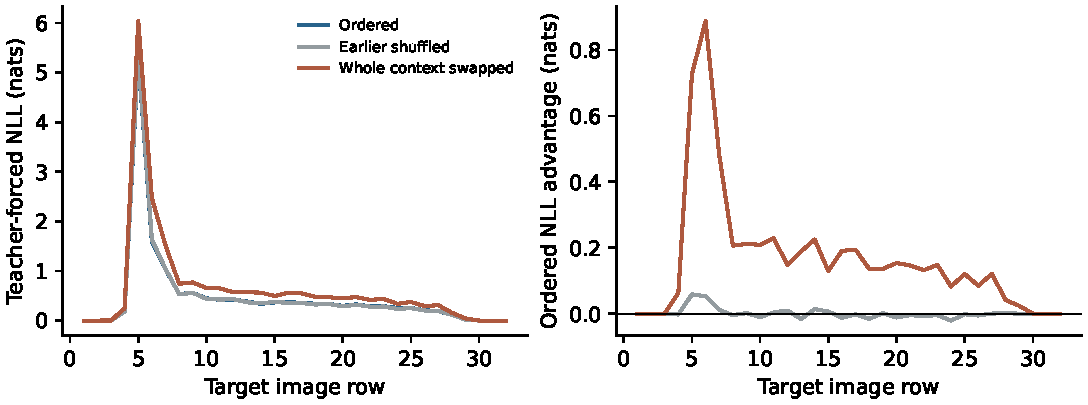
\includegraphics[width=\textwidth]{figures/Figure_S1_context_attribution.pdf}
\caption{\textbf{Exploratory row-wise attribution of raster likelihood.}
Left, teacher-forced NLL by target-image row for ordered, earlier-shuffled and
completely deranged conditions on 512 windows. Right, ordered advantage
relative to each control. Earlier target pixels are legitimately observed by
the image density, so low later-row NLL cannot itself establish language
information from the prompt. Curves are descriptive means; whole-image
uncertainty is reported in Supplementary Note 12.}
\label{fig:context-attribution}
\end{figure}

\section*{Supplementary Note 13: matched joint likelihood learning}
The joint experiment (V55) retains the exact V54 network and probability law.
Both arms initialize from its EMA, with new optimizers and EMA copies. The
frozen control trains only the 2,434,592 density parameters. The joint candidate
also trains reader parameters through the exact image likelihood, for
18,711,840 participating parameters. The unused scalar contrastive temperature
is fixed. Runtime size stays 18,711,841 in both. Reader dropout remains disabled
in both arms, independently of gradient flow. The deployed student continues
to receive and generate image tensors, without a vocabulary or external model.

Each arm makes 8,000 updates with eight streams and 16 selected causal
positions per stream, using 25\% supplied-image motor exercises. Training seed
20265510 and dataset seed 20265511 give matched new draws from the same public
corpus. Both final training-generator states match exactly. The frozen reader
is bit-identical to initialization; the joint reader changes. Reader likelihood
gradients are finite and nonzero only in the joint arm. A four-step interrupted
smoke reproduces every model and EMA tensor, plus CPU/CUDA/training RNG states.
Reader gradients cannot pass through answer-supplied motor rows because those
replace the natural state with a zero hidden vector and a fixed observed field.

The density learning rate is $2\times10^{-4}$ in both arms; joint reader rate
is $2\times10^{-5}$. Other optimizer, warmup, cosine, clipping, BF16 and EMA
settings match the earlier density experiment. The control takes
\ControlTime\ s at \ControlMemory\ GiB allocated CUDA memory; the joint arm
takes \JointTime\ s at \JointMemory\ GiB. Both run sequentially on physical
GPU 0. These costs exclude V42/V54 pretraining and data preparation.

Both checkpoints finish before either development result opens. The same
512 NLL windows, 256 generation/motor prefixes and 64 four-step feedback
streams use audit seed 20265420. Joint ordered NLL is \JointNll\ nats per
image versus \ControlNll\ for the matched frozen control. The paired gain is
\JointNllGain\ nat, interval [\JointNllLow, \JointNllHigh]. The joint-minus-control
sample identity gain is 1.172 percentage points, interval [-0.397, 2.893].
All intervals use 2,000 source-record bootstrap draws. Joint earlier-history
advantage is 0.185 nat [0.128, 0.244], versus 0.119 [0.052, 0.186] for the
continued frozen arm. Extra training accounts for part of the likelihood
progress; the matched gain isolates the reader update's additional benefit.

\section*{Supplementary Table 3: matched learning audit}
\begin{center}\begin{tabular}{lrrrr}\toprule
Arm / decoding & Identity (\%) & Exact image (\%) & Pixel F1 & Isolated ink \\
\midrule
Frozen / ordered & 2.344 & 1.953 & 0.3643 & 0.0070 \\
Frozen / shuffled & 2.344 & 1.953 & 0.3638 & 0.0071 \\
Frozen / greedy & 6.641 & 6.641 & 0.2296 & 0.0028 \\
Joint / ordered & 3.516 & 3.516 & 0.3620 & 0.0074 \\
Joint / shuffled & 3.125 & 3.125 & 0.3625 & 0.0065 \\
Joint / greedy & 7.422 & 7.422 & 0.2230 & 0.0024 \\
\bottomrule\end{tabular}\end{center}
Both arms use 256 paired prefixes and the same post-generation evaluator bank. No sampled output is selected or replaced.


Both arms preserve exact greedy copying on 256/256 targets. Stochastic-copy
F1 is 0.99993 frozen and 0.99994 joint; exact-image match is 96.875\% and
97.266\%, respectively. Joint four-step feedback identity is 3.125\% ordered
and 1.563\% shuffled; control values are 2.344\% and 2.734\%. The joint arm
passes six of eight unchanged gates, failing sampled quality and the ordered
generation advantage. The control passes five, additionally failing feedback.
The matched decision remains \texttt{\JointDecision}. Neither the primary
development reuse nor the paired intervals establish independent seed or
sealed-partition generalization.

\begin{figure}[htbp]
\centering
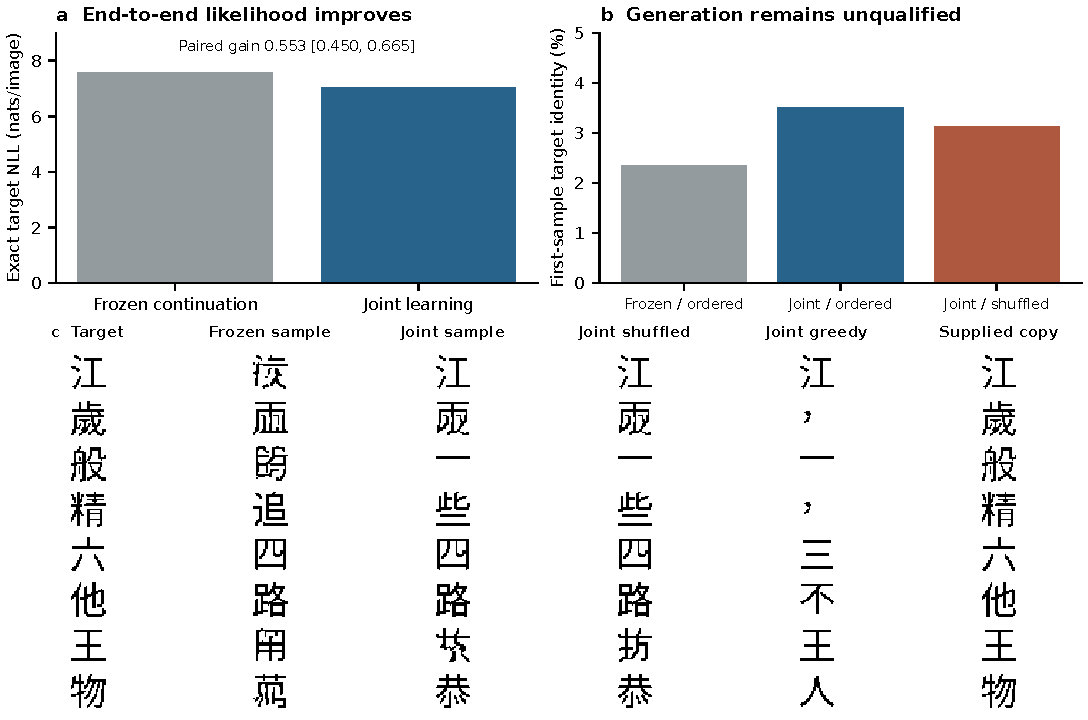
\includegraphics[width=\textwidth]{figures/Figure_S2_joint_learning.pdf}
\caption{\textbf{Matched end-to-end learning of exact raster probability.}
\textbf{a}, Joint reader--density training improves target NLL over the matched
frozen-reader continuation; annotation gives the paired source-record interval.
\textbf{b}, First-sample identity on 256 prefixes remains low under ordered
and earlier-shuffled conditions. \textbf{c}, First eight fixed audit rows:
target, frozen sample, joint sample, joint shuffled sample, joint greedy output
and answer-supplied copying. All outputs are raw model rasters, without
selection, bank replacement or OCR repair. The image panels expose errors that
the likelihood improvement alone cannot resolve.}
\label{fig:joint-learning}
\end{figure}

\section*{Supplementary Note 14: form validity after joint learning}
A post-result diagnostic compares saved images with the same 9,932 distinct
canonical rasters used for evaluation. Exact membership asks whether an output
is a known form; exact target match asks whether it equals the observed next
image. Neither uses nearest-neighbour replacement. The bank is confined to
evaluation and never enters decoding. These descriptive measurements reuse
development outputs and do not change any original decision.

Among 256 first samples, exact known-form membership rises from 9.375\% in
V54 to 33.594\% in the continued frozen arm and 43.750\% in the joint arm.
The paired joint-minus-frozen gain is 10.156 percentage points, with 95\%
source-record interval [4.219, 16.240]. Exact observed-target matches are
0.781, 1.953 and 3.516\%, respectively. In four-step feedback, joint form
membership is 46.875\% versus 38.672\% frozen; the paired gain is 8.203 points
[1.230, 14.683]. The first-sample joint greedy output has 98.438\% membership
but only 7.422\% exact target match and 34 distinct forms, compared with 78
distinct stochastic outputs. Form coherence and linguistic choice remain
separate requirements (Fig.~\ref{fig:form-validity}).

\begin{figure}[htbp]
\centering
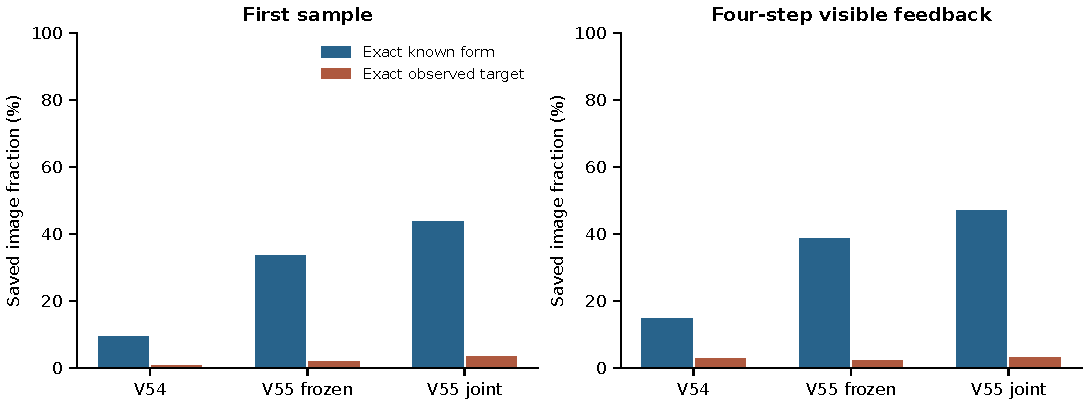
\includegraphics[width=\textwidth]{figures/Figure_S3_form_validity.pdf}
\caption{\textbf{Exact canonical form does not imply correct continuation.}
Saved first samples and four-step feedback images are compared with a fixed
canonical raster bank. Blue bars require exact pixel equality with any known
form; brown bars require equality with the observed future image. All three
checkpoints use the same bank. The paired uncertainty is stated in Note 14;
the bars are descriptive fractions, not independent replications.}
\label{fig:form-validity}
\end{figure}

\section*{Supplementary Note 15: raw-pixel beam decoding}
The V56 decoder changes search alone. V55 joint weights and the complete
binary-image law remain fixed. A beam of eight prefixes expands the next
binary pixel to ink or background, adds its exact conditional log probability
and retains the eight best scores. The row model observes preceding rows;
the masked within-row head observes preceding pixels. Parent gathering keeps
row history and row conditions aligned. Stable ties prefer ink and then the
earlier parent. Width one reproduces the original greedy rule. No persistent
glyph inventory, target identity, image replacement, rejection filter or
external model enters the decoder. Beam eight is approximate mode search,
not exact global maximization over all $2^{1024}$ images.

A two-image numerical preflight found that the original high matmul precision
gave incremental/parallel score differences above the frozen $10^{-3}$-nat
tolerance. An amendment recorded before production sets both beam and greedy
controls to highest FP32 matmul precision. It changes no weights, windows,
beam width, tolerance or quality gate. Production maximum score discrepancy
is $2.10\times10^{-5}$ nat and the width-one equality check passes.

The fixed audit uses 2,048 development windows, seed 20265620, 64 visible cells
and eight future targets. Exact next-image matches are 238/2,048 for ordered
beam, 202/2,048 for earlier-shuffled beam and 169/2,048 for ordered greedy:
\BeamAccuracy, \BeamShuffled\ and \GreedyAccuracy\%, respectively. Shuffling
preserves the final four visible cells. The paired beam-minus-greedy gain is
\BeamGain\ points [\BeamGainLow, \BeamGainHigh]; ordered-minus-shuffled is
\BeamHistoryGain\ points [\BeamHistoryLow, \BeamHistoryHigh]. Intervals use
2,000 source-record bootstrap draws, seed 20265719, with 188 source records.
All ordered and shuffled beam outputs exactly match a known canonical form.
The post-generation bank has 9,934 distinct rasters and covers every target;
it is descriptive, not the search space. Beam emits 127 distinct first forms,
versus 116 greedy. Its mean self NLL is 3.108 versus 3.508 nats/image; this
scores the selected output, not the true target, and is not a training gain.

Visible feedback uses the first 128 prefixes for eight steps. Exact observed
image matches are 68/1,024 ordered beam, 51/1,024 shuffled beam and 50/1,024
greedy. The beam-minus-greedy difference is 1.758 points [0, 3.770], with 89
source records. Adjacent image repetition is 228/896 transitions
(\BeamRepeat\%) for beam, versus one transition (\TargetRepeat\%) in the
observed streams. Shuffled beam repeats 32.366\% and greedy 17.746\%.
Mean distinct images per eight-step stream are 4.711 beam and 7.789 observed.
Thus search improves immediate conditional choice while longer output remains
repetitive (Fig.~\ref{fig:pixel-beam}). Five of six gates pass; feedback
repetition fails and the decision is \texttt{\BeamDecision}.

All 256 supplied motor images still copy exactly. The audit takes
\BeamSeconds\ s with \BeamMemory\ GiB peak allocated CUDA memory on GPU 0,
excluding previous training and data preparation. No new training or sealed
evaluation is performed. This bounded search result does not establish
question answering, instruction following, historical-script generation or
capability-matched efficiency against a text language model.

\begin{figure}[htbp]
\centering
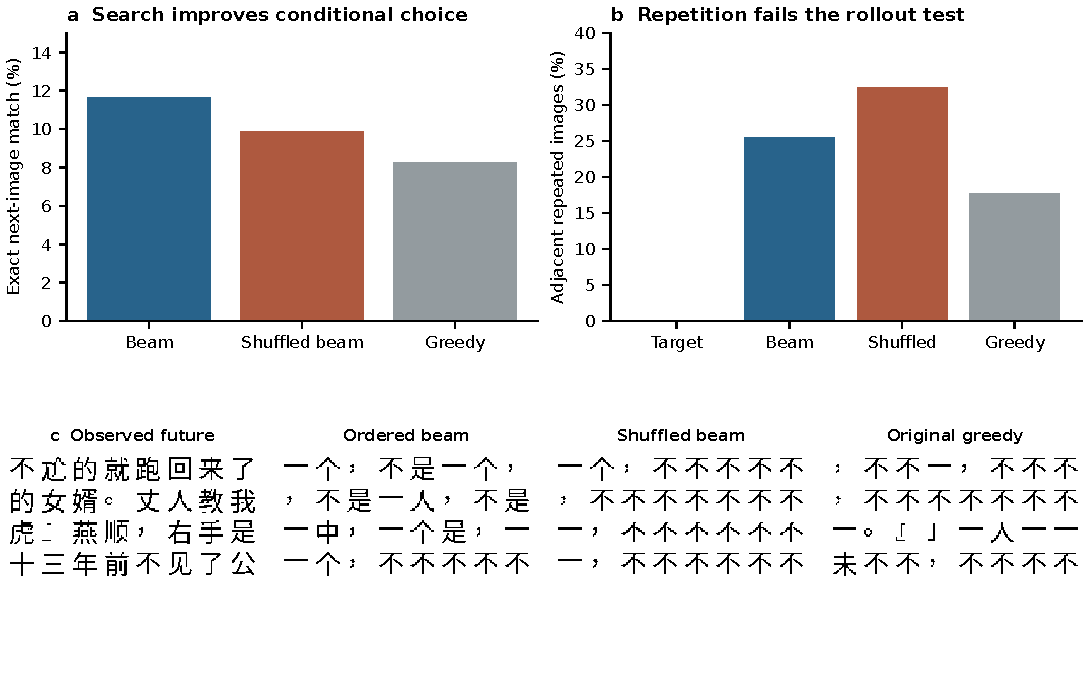
\includegraphics[width=\textwidth]{figures/Figure_S4_pixel_beam.pdf}
\caption{\textbf{Pixel search improves next-image choice but fails rollout.}
\textbf{a}, Exact target-image matches on 2,048 fixed prefixes, with unchanged
weights across ordered beam, earlier-shuffled beam and greedy controls.
\textbf{b}, Adjacent raster repetition over eight-step feedback, compared
with observed future streams. \textbf{c}, First four fixed audit streams:
observed future and raw generated images. No examples are selected or repaired.
Paired intervals are reported in Note 15; the feedback failure remains the
decoder's qualification decision.}
\label{fig:pixel-beam}
\end{figure}

\section*{Supplementary Note 16: grounded image-answer learning}
The V57 model retains the V55 joint reader and exact raster writer, extending
the allowed causal context from 64 to 512 cells. Parameter-free rotary
positions require no weight-shape change; this extension does not itself
establish trained long-context competence. Two $384\times384$ projections
produce source-position attention from the final causal query and observed
prompt states. A linear copy gate and a linear stop head give 295,682 new
parameters, for 19,007,523 runtime parameters. The contrastive temperature
remains unused and fixed. Both reader and density continue learning.

For observed source images $X_i$, attention $a_{ti}$ and copy gate
$\lambda_t$, the continued image distribution is
\begin{equation}
q_t(Y)=\lambda_t\sum_i a_{ti}\mathbf{1}[Y=X_i]
       +(1-\lambda_t)r_t(Y).
\end{equation}
Here $r_t$ is the normalized exact raster density. Duplicate source images
contribute summed mass. Equality uses lossless bit packing of observed binary
pixels; there is no persistent symbolic identity or writing bank. A query
cannot attend to source positions later than itself, including when natural
training sequences are packed together. With stop hazard $s_t$,
$p_t(\mathrm{stop})=s_t$ and
$p_t(Y,\mathrm{continue})=(1-s_t)q_t(Y)$. Training includes the terminal stop
event after a reference answer. Reference length determines supervision masks,
not a deployed input. Runtime receipts retain an inherited Bernoulli-density
description; it describes $r_t$ alone, not the complete mixture/event law.

CMRC 2018 supplies natural questions over Wikipedia paragraphs\cite{cmrc}.
Pinned source revision and original annotation offsets are checked during data
preparation. Whitespace is removed consistently, unsupported font forms are
excluded, full rendered prompts are limited to 480 cells and retained answers
to 16. No answer-centred crop is used. Answers must match the source substring
and not occur verbatim in the question. The result contains 3,211 training
questions over 1,134 paragraphs and 1,321 development questions over 421
paragraphs. Article-title and context-hash overlap are zero across splits.
The data retain CC-BY-SA-4.0 attribution. Canonical rendering and thresholding
match V55. No symbolic label is passed to a student method.

Both arms initialize from the same V55 EMA, train for 4,000 updates with batch
four and use identical data RNGs. Three of four updates draw uniform training
questions with replacement; the fourth retains 16 causal positions per natural
stream, including 25\% supplied-image motor conditions. Motor conditions use
zero hidden states and exact observed fields, bypass copying and omit the stop
loss. The no-copy arm fixes $\lambda=0$; its source-attention heads are frozen.
The first retained answer supervises event likelihood, while evaluation accepts
every retained reference. Loss is mean exact event NLL over valid image and
stop events, without the earlier image-only $1/1024$ rescaling.

AdamW rates are $3\times10^{-5}$ for the reader, $10^{-4}$ for the density and
$3\times10^{-4}$ for new heads; betas are (0.9,0.95), weight decay 0.01,
warmup 200 updates, cosine decay to 10\%, norm clip one and EMA 0.999. BF16
training uses deterministic CUDA algorithms, math SDPA and fixed cuBLAS
workspace configuration; reader dropout stays disabled. A four-update smoke
matches interrupted two-plus-two training exactly for all model/EMA tensors
and data, training, CPU and CUDA RNG states. A masked-copy backward regression
test covers matches occurring only at forbidden future positions. Copy and
no-copy training take \QaSeconds\ and \QaControlSeconds\ s, with
\QaMemory\ and \QaControlMemory\ GiB peak allocated CUDA memory on GPU 0.
These costs exclude previous foundation training and preparation.

Both final EMA checkpoints complete before development opens. Primary IDs are
256 samples without replacement from sorted development records, seed
20265720. The decoder stops at hazard $\geq0.5$; otherwise it selects the copy
component at gate $\geq0.5$, sums attention over equal observed rasters and
emits the largest-mass image. The free component uses pixel beam eight. This
is hierarchical greedy decoding, not global mixture-mode search. The 17-cell
safety cap is recorded separately from stopping. No answer location, reference
length or candidate answer list is available at inference.

Exact answer match requires every output image, its order and learned stop to
match a retained reference. Raster F1 measures multiset overlap of exact
rasters, maximizing over references. It can credit reordered images and is
not the official word-segmented CMRC metric. Primary copy exact match is
10/256 (\QaExact\%), versus 1/256 with question pixels blanked and 0/256 no-copy. Copy F1 is
\QaFone\%, versus \QaBlankFone\% and \QaControlFone\%. Its paired gain over
blanking is \QaQuestionGain\ points [\QaQuestionLow, \QaQuestionHigh]; over
no-copy it is 9.136 [5.879, 12.483]. Intervals use 2,000 source-article draws,
seed 20265819, retaining related questions together (198 primary articles).
The blanking intervention removes question ink while retaining passage and
framing; it is not an in-distribution alternative natural question.

All 393 shared-paragraph/disjoint-answer question pairs are also tested.
Only one has both answers exactly correct (\QaPairExact\%). Mean primary
answer length is 10.457 cells, and 58/256 cases reach the safety cap.
Every primary copy-arm image uses copying, with no free-branch emission.
Teacher-forced mean event NLL across all 1,321 development questions is
1.329 copy versus 12.025 no-copy; mean sequence NLL is 8.377 versus 91.477.
All 256 V55 supplied motor images remain exact. The full audit takes
1,117.1 s and peaks at 0.140 GiB allocated CUDA memory, including the slower
2,106-image free-writing control. Four of seven gates pass: boundary, clean
split/resources, motor and question-dependent F1. Exact answers, absolute F1
and paired-question correctness fail. The decision is \texttt{\QaDecision}.

A post-result, zero-model-call diagnostic on the saved primary outputs finds
43/256 correct first images. Only 10/43 of those become exact complete answers;
14/256 outputs contain a complete reference prefix followed by unwanted
additional images. Mean aligned correct prefix length is 0.750 cells; adjacent
repetition is 2.230\%. These descriptive observations do not alter the locked
decision. They motivate testing answer-level structure alongside better
evidence selection. All results remain limited to canonical, answerable,
short-paragraph reading; independent seed replication, raw page segmentation,
historical writing and general language generation are unestablished.

\section*{Supplementary Note 17: complete observed image blocks}
V58 continues the completed V57 copy EMA with a normalized distribution over
all contiguous observed prompt blocks $X_{i:j}$, where $1\leq j-i+1\leq16$.
For causal states $h_i$ and final prompt state $h_L$, define
\[
 s_{ij}=\frac{(W^s_qh_L)^\top W^s_kh_i+
                   (W^e_qh_L)^\top W^e_kh_j}{\sqrt{384}}+b_{j-i+1},
 \qquad \pi_{ij}=\frac{e^{s_{ij}}}{\sum_{uv}e^{s_{uv}}}.
\]
The answer-image law is
\[
 p(Y\mid X)=\sum_{ij:\,X_{i:j}=Y}\pi_{ij}.
\]
Equality is lossless raster equality, computed from binary pixels; indices
address only the current prompt. There is no persistent glyph inventory.
Training minimizes exact negative log block mass, divided by reference cell
count plus one boundary event across the batch. Annotated source offsets do
not enter the loss. Mode decoding sums mass over equal sequences and chooses
the most probable sequence, with first-source tie breaking. No reference
length, answer list, OCR or output repair enters generation. The predicted
end boundary terminates a nonempty block; the 16-cell support is fixed before
training. The retained copy/free/stop continuation path remains separate.

Four new 384-by-384 projections and sixteen length biases bring the runtime
to 19,597,363 parameters. Projection pairs initialize from V57 copy attention;
the matched glyph control constructs and freezes the same new heads. Both
start from identical V57 copy EMA weights and make 4,000 updates, batch four,
using the previous three-to-one QA/natural-motor schedule, optimizer rates
and deterministic settings. Seeds are 20265810 (training) and 20265811 (data).
A four-update uninterrupted versus two-plus-two resumed GPU run matches all
model/EMA tensors and data, training, CPU and CUDA RNG states exactly.
Block training takes 210.995 s, 0.967 GiB peak allocated memory; the glyph
control takes 302.237 s, 1.056 GiB. Earlier foundation costs are excluded.

Both final checkpoints precede development inspection. Primary IDs are the
same 256 as V57, explicitly reused development, not a sealed final test.
Exact answers are 25/256 (9.766\%) block, 3 blank-question and 21 matched glyph control.
F1 is 27.033\%, 9.169\% and 22.140\%. Article-grouped bootstrap uses 2,000
draws, seed 20265919. Block-minus-control F1 is 4.893 points [0.469, 9.047];
exact match is 1.563 [-1.509, 4.652]. Normal-minus-blank F1 is 17.864
[13.438, 22.289]. Only 4/393 pairs have both answers correct; the paired gate
fails and the registered decision remains \texttt{reject\_reading\_model}.
All 256 supplied motor images remain exact. Mean conditional block sequence
NLL is 6.505, versus 9.552 for glyph-event sequence likelihood; these laws have
different supports and must not be treated as interchangeable language
perplexities. The audit takes 98.951 s at 0.142 GiB allocated memory.
The 78,772,107-byte inference-only export reproduces native prompt-PNG
answers and events exactly. Raw first audit failures appear in Figure 5.

\section*{Supplementary Note 18: frozen visual foundation probe}
V59 pins MIXAR-477M stage-2 revision
\texttt{c5d5bcfbad2f290296fd83810558f396c6a6333a}, reusing its shared
Apache-2.0 checkpoint. Author-reported multilingual pretraining and its
four-H200 compute are external work, not part of single-4090 training here.
Both it and the frozen V58 reader consume identical Noto CJK 26-pixel glyphs
inside binary 32-pixel cells. This differs from MIXAR's native rendering.
An odd-length prompt gets a blank final cell for two-cell pairing; readout
candidates exclude that extra cell. Both encoders supply states after each
complete pair, repeated over its two source cells.

A fixed CPU-QR semi-orthogonal projection maps MIXAR's 896 states to 384
coordinates, seed 20265900; student states already have width 384. Both append
128 projected normalized-DCT coordinates, seed 20265901, plus two within-pair
phase channels. Semantic and fine-image parts are separately RMS-normalized.
The 514-dimensional features are quantized to FP16 for caching and readout.
All train, development and blank-question features are prepared without
reading answer annotations. Recomputed quantized features agree exactly.

Each fresh head has four 514-to-384 projections and sixteen biases, totaling
789,520 learned parameters. Both train 4,000 updates, batch eight, with seeds
20265910/20265911, AdamW rate $3\times10^{-4}$, betas (0.9,0.95), decay 0.05,
norm clip one, warmup 200, cosine to 10\%, and EMA 0.999. Frozen encoders and
native free writers are unchanged. An interrupted/resumed GPU preflight
matches weights, EMA and RNG states exactly. Features take 184.781 s and
1.906 GiB; student and MIXAR readouts take 106.593 and 109.257 s, each at
0.170 GiB. These resource numbers exclude external pretraining.

Both completed heads precede inspection of the same reused 256 development
IDs and 393 pairs. Student exact/F1 scores are 9.375/25.340\%; MIXAR scores
2.344/11.588\%. MIXAR-minus-student F1 is $-13.752$ points
[$-18.247$,$-9.094$], using 2,000 article draws, seed 20266019.
Normal-minus-blank F1 is 2.246 [0.415,4.378] for MIXAR, versus 18.343
[13.949,22.519] for the student. Both questions are exact in zero versus
twelve pairs. Three of seven gates pass; the frozen-foundation probe fails.
The 117.085-s, 0.094-GiB audit uses cached readouts and excludes online encoder
inference. Figure S5 reports all four conditions. Capacity, pretraining,
prior task training and rendering differ; this is a scoped foundation probe,
not a general ranking of encoders or native-font MIXAR competence.

\plate{Figure_S5_frozen_foundations}{\textbf{Frozen pretrained features do not
improve this reading interface.} Identical learned block heads consume frozen
student or MIXAR features, with normal and blank-question prompts. All scores
use the fixed 256 questions. External pretraining and rendering shift prevent
a causal attribution to capacity or pretraining alone.}{fig:frozen-foundations}

\section*{Supplementary Note 19: question-first causal reading}
V60 tests whether passage states should be conditioned on the question before
evidence selection. The context-first host layout places passage $X$ before
question $Q$; the intervention reverses these two blocks, yielding causal
passage states $h_i=f(Q,X_{\leq i})$. Framing and total visible length are
unchanged. Both models start from identical V58 block EMA weights and retain
the 19,597,363-parameter architecture, block law, image-only supervision,
mode decoder and continuation writer. All visible prompt positions remain
candidates. There is no answer offset or answer-aware cropping.

Each arm makes 4,000 updates with the same V58 batch-four schedule, optimizer
rates, warmup, cosine, clipping, EMA and deterministic BF16/math-SDPA regime.
Training/data seeds are 20266010/20266011. The new prompt-order helper is
tested for exact preservation of source characters and correct blanking
positions. An uninterrupted versus two-plus-two resumed GPU preflight
matches all model/EMA tensors and RNG states exactly. Both production arms
finish before their development scores open. Context-first and question-first
training take 214.699 and 225.207 s, each at 0.966 GiB peak allocated CUDA
memory. Cost remains incremental to the same previously trained foundation.

The same 256 primary IDs and 393 paragraph pairs are explicitly reused.
Question pixels are blanked at each arm's actual question positions, retaining
the paragraph, length and framing. Exact answers are 27 context-first and
21 question-first, versus three and two for the corresponding blank controls.
F1 is 26.908\% and 23.765\%, versus 7.572\% and 9.098\% blanked. With 2,000
article-grouped bootstrap draws, seed 20266119, question-first minus
context-first F1 is $-3.143$ points [$-6.544$,0.446]; exact match is
$-2.344$ [$-5.490$,0.810]. Neither difference resolves zero. The question-first
normal-minus-blank F1 gain is 14.667 [10.873,18.809]. Both answers are exact in
5/393 question-first pairs, versus 16/393 context-first pairs.

All 256 supplied motor images remain exact for both arms. The complete audit
takes 192.723 s at 0.184 GiB allocated CUDA memory. Four of eight registered
gates pass: boundary, clean split/resources, question-dependent F1 and motor.
The gain, absolute accuracy, absolute F1 and paired-question gates fail, so
the decision is \texttt{reject\_question\_first\_intervention}. This is one
matched training seed and a task-trained, context-first foundation; neither a
universal ordering result nor a final generalization test is established.

\plate{Figure_S6_question_first}{\textbf{Changing input order is insufficient.}
Matched models receive the same source writing with the question before or
after the passage. Question blanking uses each layout's actual positions.
The question-first F1 difference is unresolved and its registered reading
criteria fail.}{fig:question-first}

\section*{Supplementary Note 20: full native pixel-language adaptation}
The complete released MIXAR-477M\cite{mixar} image-language model is adapted
using the pinned release identified by its full revision, weight SHA-256 and
architecture-code hashes in the accompanying evidence. This is
supervised adaptation of external pretraining, not local foundation training
from scratch. All 477,145,984 contextual and image-output parameters train.
The source data are the same 3,211 training and 1,321 development questions
used for the preceding reading experiments, with no article or context-hash
overlap. Development is explicitly reused. Complete prompts contain at most
480 cells and first-reference training answers at most 16 cells.

Noto CJK glyphs at 26 pixels occupy 32-pixel binary cells, a rendering shift
from the author's native bundled-font interface. Odd prompt/answer lengths
receive one blank cell for alignment to 32-by-64 native blocks. Two all-white
blocks follow each target answer. Native input uses white $+1$ and ink $-1$;
the target Bernoulli probability describes white pixels. Spatial prompt bounds
are known, but strings, codepoint IDs and source-answer offsets never enter
the actor. The causal answer-only objective is
\begin{equation}
\mathcal L=-\frac{1}{|A|P}\sum_{t\in A}\sum_{i=1}^{P}
\left[y_{ti}\log\sigma(a_{t-1,i})+(1-y_{ti})\log(1-\sigma(a_{t-1,i}))\right],
\end{equation}
where $P=2048$, $A$ contains answer and termination blocks, and state $t-1$
depends only on preceding physical images. Prompt labels contribute no loss.

The registered run uses 1,000 updates, microbatch one accumulated eight times,
uniform replacement sampling, AdamW $2\times10^{-5}$, betas $(0.9,0.95)$,
weight decay 0.01, warmup 50, cosine decay to 10\%, norm clip one and EMA
0.99. Seeds are 20266110 for training and 20266111 for data. FP32 weights,
optimizer and EMA coexist with BF16 forward/backward, deterministic algorithms,
math attention and nonreentrant activation checkpointing. The final EMA is
used without development checkpoint selection. A real four-update interrupted
preflight reproduces model, EMA, optimizer and all RNG states exactly, with
finite gradients throughout. Altering future answer pixels changes earlier
logits by exactly zero in the recorded causality check.

Training through the final update takes 1,501.138 s, with 9.912 GiB peak
allocated memory; loading takes 2.525 s. Cache preparation, final serialization
and external pretraining are separate. All work uses physical GPU 0. Greedy
decoding thresholds each white logit at zero, feeds back the generated image
and stops at the first exactly white block, otherwise capping at ten new
blocks. Only terminal blocks and entirely blank trailing cells are removed.
No malformed image is repaired or snapped to a character.

The locked audit compares adapted and released-base actors with normal and
blank-question inputs on the same 256 primary IDs, and tests all 393
shared-paragraph question pairs for the adapted actor. All 1,321 development
examples contribute likelihood. Pixel NLL decreases from 0.684156 to
0.154814 nats, yet exact answers are zero and exact-raster multiset F1 is
0.149\%. Foreground F1 is 12.264\%, compared with 8.473\% blanked and zero
for the released base under this shifted interface. Article-grouped bootstrap
with 2,000 draws, seed 20266219, gives the adapted-minus-blank foreground
difference as 3.791 points [2.521,5.056]. The exact-raster F1 difference is
0.149 [0,0.372], unresolved. Both-correct pair accuracy is 0/393.

No primary output is empty or capped for the adapted actor; the released base
returns an empty answer on every normal primary prompt. The adapted mean
length is 3.047 cells. Five of ten gates pass: image-only runtime, clean
split/finite resources, full backward/resume/causality, independent replay,
and capped-output rate. Exact answers, raster F1, adaptation gain,
question-dependent raster F1 and paired correctness fail. Audit time is
145.690 s excluding loading, at 1.832 GiB allocated memory. The registered
decision is \texttt{reject\_native\_free\_reading}.

A learned-weight deployment bundle includes configuration and local custom
architecture code. A fresh offline process with empty model and code caches
reproduces actual answer tensors, PNG bytes and stopping events. It loads no
original release weights and calls no external model, tokenizer or OCR.
Exact replay is an implementation result, separate from language quality.

An auxiliary transcription plan was registered before development outputs
were inspected. CPU Tesseract 5.3.4 receives anonymous answer-only images,
enlarged fourfold with a white margin, without questions, references or model
names. It recognizes only 40/256 retained reference images exactly, a 15.625\%
calibration rate. No generated answer is transcribed exactly, but the poor
reference calibration precludes treating this as a reliable semantic score.
The primary raw-image failure and strict gates remain unchanged. One seed,
the shifted font interface, limited training data and absent general-language
evaluation constrain the interpretation.

\section*{Supplementary Note 21: conditional whole-image density}
The matched experiment tests a latent expert shared across a complete native
image block. Let $h_t$ be the visual transformer's causal state after the
visible prefix and let $y\in\{0,1\}^{2048}$ denote the next $32\times64$
bitmap, with one denoting white in this native interface. The normalized law is
\begin{equation}
 p_\theta(y\mid h_t)=\sum_{k=1}^{K}\pi_{\theta k}(h_t)
 \prod_{i=1}^{2048}q_{\theta ki}(h_t)^{y_i}
 [1-q_{\theta ki}(h_t)]^{1-y_i},
 \qquad q_{\theta ki}=\sigma(a_{\theta ki}),
\end{equation}
where the gate is a softmax. Each expert is a neural function of the current
visual state, without a fixed character identity or stored target bitmap.
Marginalizing the expert retains a proper probability law. For distinct
pixels, conditional covariance is
\begin{equation}
 \operatorname{Cov}(Y_i,Y_j\mid h_t)
 =\sum_k\pi_k q_{ki}q_{kj}
 -\Bigl(\sum_k\pi_k q_{ki}\Bigr)\Bigl(\sum_k\pi_k q_{kj}\Bigr).
\end{equation}
It can be nonzero even though pixels are independent within one expert.
This elementary property permits coherent alternatives; it does not prove
that training discovers valid writing or useful answers.

The objective is exact negative log joint likelihood, computed with
\texttt{logsumexp}, divided by 2,048 physical pixels. It averages only
answer and two blank termination blocks within each example, then averages
over accumulated examples. Teacher forcing uses the same one-block causal
shift as Note 20. Prompt pixels enter the context without a prompt loss.
There is no transcript, answer-span offset or Unicode target inside the actor.

The single-head control has 477,145,984 parameters; eight experts have
489,998,208. Both initialize from the same externally pretrained MIXAR
revision and use the unchanged Noto-26 cell interface, 3,211 training
questions and 1,321 article-disjoint development questions. The eight-head
projection repeats the released head with zero-mean perturbations of scale
0.01, seed 20266210, and a zero-initialized gate. Every backbone and head
parameter receives gradients. The comparison matches examples, optimization
and update budget, rather than parameter count or output computation.

Each arm uses 1,000 updates, microbatch one, accumulation eight, AdamW at
$2\times10^{-5}$ with betas $(0.9,0.95)$, decay 0.01, 50-update warmup,
cosine decay to 10\%, norm clip one and EMA 0.99. Weights, optimizer and EMA
are FP32; forward/backward use BF16 with deterministic algorithms, eager/math
attention and nonreentrant activation checkpointing. Training and data seeds
are 20266220 and 20266221. Complete sampled-example orders must match exactly.
Only the final EMA is audited. Both arms run sequentially on physical GPU 0,
under a 20 GiB allocated-memory and four-hour ceiling per phase.

Generation thresholds each expert into one complete candidate bitmap, scores
all candidates under the full mixture and emits the highest-scoring candidate.
Searching component modes is approximate MAP; it is not a guarantee of the
global mixture mode. Actual emitted pixels become subsequent context. The
first exactly white native block ends generation, otherwise ten blocks cap
the continuation. Only the detected terminal block and wholly blank trailing
cells are removed. Malformed nonblank strokes are preserved. The deployed
bundle has no tokenizer, OCR, glyph inventory or external language-model call.

The primary audit retains the fixed 256 questions, blank-question controls,
all 393 shared-paragraph pairs and all-development likelihood. Paired
intervals resample articles 2,000 times, seed 20266229. An intervention pass
requires positive lower intervals for both K8-minus-K1 strict-raster F1 and
K8 normal-minus-blank F1, fewer than 20\% capped outputs and all implementation
checks. Each arm's separate bounded reading gate requires at least 10\%
exact answers, 25\% raster F1, 2\% both-correct pairs, a positive question
effect, fewer than 20\% caps and implementation checks. Expert-use counts
and gate entropy are descriptive; they cannot select a new checkpoint or
change these gates. Reused development, one seed, the shifted font interface
and external pretraining limit the conclusions.

Both arms complete their registered budget and all replay checks. K=1 takes
1,887.5 s at 9.904 GiB peak allocated memory; K=8 takes 1,972.8 s at 10.174 GiB.
Their complete training-example orders match exactly. The locked audit takes
527.4 s excluding model loading, at 1.904 GiB allocated memory. Four-update
uninterrupted versus two-plus-resumed-two preflights match model, EMA,
optimizer and every RNG state exactly for each arm. Future-pixel changes
have zero effect on earlier predictions. Strict-FP32 cache errors remain
below $2.1\times10^{-5}$; larger TF32 discrepancies are retained separately
rather than hidden by changing the production recipe.

All-development NLL is 0.1542 for K=1 and 0.1248 for K=8. Primary strict-raster
F1 is 0.234\% versus 0.815\%, a 0.580-point gain [0.089, 1.094]. Foreground
F1 is 12.205\% versus 15.827\%, a 3.623-point gain [1.815, 5.554]. Both
arms have zero exact primary answers and zero both-correct pairs. K=8's
normal-minus-blank raster difference is 0.295 points [$-0.006$, 0.623]; its
foreground difference is $-0.044$ points [$-0.629$, 0.509]. Neither resolves
question dependence. Seven of eight intervention gates pass; both arms pass
six of ten bounded reading gates. The registered decision is
\texttt{reject\_density\_intervention}; neither arm qualifies as free reading.

K=8 selects experts 0, 1, 2, 4 and 7 on respectively 223, 4, 106, 605 and 3
primary generation steps, including termination. Mean gate entropy is 1.812
nats, compared with $\log 8=2.079$ for a uniform gate. The primary outputs all
terminate before the cap, while one blank-question output reaches the cap.
These descriptive observations do not identify semantic expert roles or
justify selecting different parameters. The result supports improved bitmap
fit at this budget, while the required question-dependent language remains
unestablished.

\subsection*{Auxiliary reader and post-hoc transcript sensitivity}
A separately preregistered, answer-only Qwen3-VL 8B reader transcribes
122/128 training-reference images exactly (95.313\%), returns every one of
16 blank and 16 random-ink controls empty, and produces valid JSON throughout
calibration. The fixed instruction and anonymous images disclose neither
questions nor reference answers to the reader. Three responses among 1,015
unique actor images are invalid, including two that reach the registered
256-output-token limit. The original diagnostic therefore reports
\texttt{invalid\_actor\_transcription}; it has no complete fixed-case score.

An explicitly post-hoc sensitivity analysis reuses the first responses
without retry, repair or new model calls. It retains all 256 cases in each
condition and assigns each invalid bounded score possible range $[0,1]$.
The resulting full-case means are below; ranges are identification intervals,
not confidence intervals. Exact text means normalized transcript agreement
with any retained reference. Character score is one minus normalized edit
error, clipped to $[0,1]$.
\begin{center}\small
\begin{tabular}{lrrr}\toprule
Condition & Valid / unknown & Exact text (\%) & Character score (\%)\\\midrule
K=1 & 254 / 2 & 0.781--1.563 & 1.388--2.169\\
K=1, blank Q & 255 / 1 & 0.000--0.391 & 0.186--0.577\\
K=8 & 256 / 0 & 0.000 & 2.806\\
K=8, blank Q & 256 / 0 & 0.000 & 2.945\\
\bottomrule\end{tabular}
\end{center}

K=8's normal-minus-blank character difference is $-0.139$ percentage points,
with article-bootstrap sensitivity envelope [$-0.962$, 0.638]. The envelope
uses 2,000 article resamples, seed 20266379, taking the lower endpoint's
2.5th percentile and upper endpoint's 97.5th percentile. It covers the
unknown-score assignments within this resampling scheme, not systematic
reader errors, training-seed variation or reused-development selection.
It establishes no new model qualification and changes neither failed decision.
The external reader makes 1,172 calls over 1,092.1 s of owned runtime including
cleanup; maximum resident GPU memory sampled after requests is 7,278 MiB.
These costs are separate from actor inference and training. The evaluator
server and runner exit, its port closes and GPU 0 memory is released.

\section*{Supplementary Note 22: matched question--answer assignment}
For two observed question images $x_0,x_1$ about the same paragraph and two
accepted answer-image streams $y_0,y_1$, define $e_{ij}$ as mean answer and
termination-pixel NLL for $y_j$ conditioned on $x_i$. Each actor scores all
four streams using the complete image generator. Let
\begin{align}
 D &= e_{01}+e_{10}-e_{00}-e_{11},\\
 \mathcal L_{\mathrm{positive}} &= (e_{00}+e_{11})/2,\\
 \mathcal L_{\mathrm{assign}} &= \tau\log(1+\exp[-D/\tau]),\qquad \tau=0.01,\\
 \mathcal L &= \mathcal L_{\mathrm{positive}}+\lambda\mathcal L_{\mathrm{assign}}.
\end{align}
Aligned uses $\lambda=1$ and control $\lambda=0$. Additive question-only and
answer-only energy offsets cancel from $D$. Different answer lengths receive
their own normalization, so $D$ is not a joint log-odds or mutual-information
estimate. The algebra does not identify linguistic meaning.

There are 3,793 training-only pairs from 939 paragraphs and 3,016 questions.
Accepted answer text sets and canonical reference images are distinct within
each pair; two pairs with shared references are excluded. Sampling chooses
paragraphs uniformly, then a pair within the paragraph. Both actors start
from the same learned V62 eight-expert EMA, retain 489,998,208 parameters and
use the unchanged Noto-26 interface and approximate component-mode decoder.
No reference bank, OCR or teacher is deployed. All 2,000 update journals,
containing four pair draws each, match byte for byte.

Microbatch is one pair with accumulation four. Each pair forms two positive
and two swapped likelihood streams. AdamW uses learning rate $2\times10^{-5}$,
betas $(0.9,0.95)$, decay 0.01, 100-update warmup, cosine decay to 10\%, clip
one and EMA 0.99. Model/optimizer/EMA weights are FP32; forward/backward use
BF16, deterministic eager/math attention and nonreentrant checkpointing.
Model and data seeds are 20266320 and 20266321. Only final EMA is audited.
Both arms execute sequentially on physical GPU 0 under eight-hour and
20-GiB allocated-memory ceilings per phase.

\begin{table}[htbp]\centering\small
\caption*{\textbf{Supplementary Table 4: completed question--answer assignment.} Image F1 values are percentages.}
\begin{tabular}{lrrrr}\toprule
Arm & Exact / 256 & Raster F1 & Foreground F1 & Both / 393\\\midrule
Control & 2 & 3.229 & 20.227 & 0\\
Aligned & 1 & 2.417 & 17.219 & 0\\\bottomrule
\end{tabular}
\end{table}

Control and aligned all-development NLLs are 0.113901 and 0.114186 nats per
pixel. Aligned minus control raster F1 is $-0.812$ points [$-1.504$,$-0.202$];
foreground F1 differs by $-3.008$ points [$-3.978$,$-2.014$]. Normal-minus-blank
raster effects are 1.765 points [0.504,3.251] for control and 1.677
[0.492,3.033] for aligned. All intervals resample source articles 2,000 times,
seed 20266329, over the same 256 primary cases from 198 articles.

Each actor passes seven of ten reading gates. Both fail the unchanged 10\%
exact-answer, 25\% raster-F1 and 2\% both-correct-pair requirements. Question
dependence, capped outputs and implementation checks pass. The intervention
requires an aligned reading pass and a positive lower interval for
aligned-minus-control raster F1; both requirements fail. The decision is
\texttt{reject\_assignment\_intervention}. No decoder, checkpoint selection,
threshold or primary case changes after scoring.

The separate accepted-reference diagnostic assigns the pair correctly in
324/393 cases for control and 330/393 for aligned. Both individual energy
ranks are correct in 82/393 and 109/393. These are descriptive comparisons
without registered difference intervals, and do not evaluate free writing.
Training takes 7,355.156 and 6,737.336 s at 10.301 GiB peak allocated memory.
The audit takes 582.104 s excluding loading, at 1.904 GiB. Timing excludes
loading, final serialization and external foundation pretraining.

The preflight passes exact uninterrupted/resumed optimizer, EMA and RNG
comparison, finite complete-backbone and assignment-only gradients, causal
masking and physical stream assembly. Largest-pair allocation is 9.197 GiB.
Same-shape future-pixel effects are zero; strict-FP32 cached-prefix error is
$6.485\times10^{-5}$ against a $2\times10^{-4}$ bound. Both standalone bundles
reproduce tensors, PNG bytes and stopping events with networking disabled,
empty caches and no repository source path. Reused development, one seed,
external pretraining and strict-raster limitations remain explicit. Sealed
final partitions are unopened.

\section*{Supplementary Note 23: inherited continuous writing actor}
A separately executed successor retains the existing authenticated Qwen3-VL
vision/contextual archive\cite{qwen3vl}, omits its vocabulary matrices and
attaches a continuous physical-image writer (Fig.~\ref{fig:grounded-actor}).
It has 7,548,043,521 parameters: 7,522,463,984 inherited/frozen and 25,579,537
trainable. The trainable subset includes rank-eight query/value/output
adapters in 36 contextual layers, two continuous writing queries, a
19,374,096-parameter six-layer flow writer and a binary stop classifier.
All 27 vision layers and three DeepStack feature sets remain present.
The actor accepts observed grayscale image tensors and completed
$32\times64$ blocks; it requires no character segmentation or alphabet.

Teacher forcing places each query pair before its answer image. The observed
prompt may be bidirectionally image-encoded, while each completed answer block
is an independent encoder image. A causal contextual mask prevents current
and future answer pixels from entering a prediction. Cached generation
rereads only completed generated blocks. Explicit spatial/temporal rotary
coordinates preserve image layout; sequential mask coordinates carry no
character identity.

The writer models all 2,048 pixels jointly. With Gaussian $U$, uniform $t$ and
signed target image $Y$, its flow objective is
\begin{equation}
 Y_t=(1-t)U+tY,\qquad
 \mathcal L_{\mathrm{flow}}=\mathbb E\Vert v_\theta(Y_t,t,h)-(Y-U)\Vert_2^2.
\end{equation}
Explicit midpoint integration gives a continuous raster; zero thresholding
produces binary output. A class-balanced binary stop objective is separate
from white-space generation. Its sigmoid score has no independent calibration.
No token IDs, OCR, font renderer, glyph bank or external model call enters
actor inference. Encoded text remains permissible in offline dataset creation.

All 19 complete-model execution checks pass on GPU 0 at 17.181 GiB allocated
and 18.053 GiB reserved peak memory. Geometry inspection covers 12,976 complete
training examples from CMRC and Dolly instructions\cite{cmrc,dolly}. The
largest contextual case has 918 positions, a $480\times1024$ prompt and
109 complete target blocks; the largest prompt is $512\times1024$.
Both receive full contextual backward with Adam moments allocated, while
16 uniformly sampled target blocks receive writer loss. No prompt or
answer history is truncated. Every trainable gradient is finite, and
nonzero gradients reach first/last contextual adapters and the writing head.
Restoring one saved optimizer update reproduces the next writer/adapters,
optimizer, sampling and global RNG states exactly. Same-shape future-image
and encoder-isolation interventions have exactly zero effect.

Two retained attempts fail cached/full-prefix comparison at relative maximum
errors 0.18524 and 0.09815. The accepted implementation keeps contextual weight
storage in BF16 but evaluates contextual projections, attention and residuals
in FP32. Layer checkpointing avoids retaining a full FP32 body. Vision
weights/computation are FP32; writer contractions may use BF16 autocast.
The complete contextual call disables ambient autocast, verified at actual
attention entry. Cached/full-prefix error becomes $3.910\times10^{-4}$
absolute and $1.210\times10^{-5}$ relative, below the unchanged 0.02 relative
bound. These casts do not recover precision lost in the source quantization.

A separate offline helper temporarily reads source token rows and an output
head to test the contextual initialization against the source engine. Across
eight short text-only prompts, it matches 8/8 initial and 9/9 returned token
choices, with mean KL 0.000264 nat after grouping reference top-ten tokens
and the outside mass. This limited check is not full engine equivalence or
image-language understanding. The helper vocabulary is never attached to
the actor, and its owned reference service exits before native model loading.
Its 103.832-s runtime and 18.701-GiB allocation include the temporary head
and are separate from the image-actor preflight.

The preflight contains two optimizer updates and replay; its output is noise.
It provides no writing or language quality score. A separate writer-only
curriculum then trains 19,374,096 parameters for 10,000 updates on balanced
Chinese/English blocks from 12,976 training examples. With the final EMA fixed,
128 development blocks yield foreground F1 of 34.000\% under correct visual
conditions and 21.420\% with cyclically shuffled conditions, a gain of 12.581
percentage points. Neither route produces an exact block. Both registered
component requirements, F1 at least 90\% and gain at least 20 points, fail.
Training peaks at 15.801 GiB; the resumed evaluation's separately reset peak
is 15.514 GiB. The first evaluation attempt stops before output because its
directory is missing. Creating that directory and resuming unchanged code at
update 10,000 leaves final weights and training journals byte-identical, with
no further learning. All 256 generated-image scores are recomputed from raw
pixels. These are source-image reconstruction measurements on reused
development data, not prompt-to-answer language. Independent autonomous
answers, historical-form behavior and capability-matched efficiency remain
required. External pretraining is inherited work, not training performed
from scratch on the local GPU.

\plate{Figure_S7_grounded_actor}{\textbf{An inherited image actor executes within one GPU, with language quality unqualified.}
Observed prompt images and independently encoded completed blocks enter the
retained visual/contextual body. Two continuous queries condition a flow over
physical writing pixels. Blue modules contain trainable components; the
contextual body also retains frozen inherited weights. A separate classifier
predicts stopping. Parameter counts and memory describe actual complete-model
execution. The diagram contains no generated-language example or quality claim.}{fig:grounded-actor}

\section*{Supplementary Note 24: matched writer-fitting diagnosis}
The failure in Note 23 motivates a factorial experiment on 64 fixed training
blocks. Each block is a physical $32\times64$ crop, which can contain partial
letters or characters. Conditions are either the inherited reader's two
4096-dimensional features or a lossless embedding of the actual target
pixels. The latter is an answer-supplying oracle control. Each condition is
crossed with Gaussian velocity learning or direct one-pass image MSE, using
the same writer architecture, initialization and 2,000-update batch exposure.
All four early optimizer/EMA/RNG replays pass.

\begin{center}\small
\begin{tabular}{lrrr}\toprule
Condition / objective & F1 (\%) & Exact / 64 & Shuffled F1 (\%)\\\midrule
Reader / flow & 34.567 & 0 & 26.716\\
Reader / direct & 99.995 & 63 & 27.466\\
Pixels / flow & 33.648 & 0 & 26.581\\
Pixels / direct & 100.000 & 64 & 27.464\\\bottomrule
\end{tabular}
\end{center}
All 512 main generated-image scores and all 8,000 batch draws are independently
verified against the original training pixels. The fitting result rejects an
immediate flow-writing explanation at this configuration; it does not prove
generalization from inherited features. Source-feature extraction peaks at
15.251 GiB. Subsequent writer fits peak near 0.66 GiB after the unused semantic
body is released, so the latter is not complete language-model memory.

An auxiliary native-codec comparator initially uses the wrong image polarity,
giving F1 81.364\%. That original report is retained and invalidated. The
codec was trained with white-positive input. A separately recorded correction
using its actual convention reconstructs all 64 training images exactly.
Both comparator outputs and the correction are independently verified. The
fixed raw rows in main-text Fig.~9 remain unmodified.

\section*{Supplementary Note 25: broad direct writing and a fixed output codec}
The broader direct writer retains the full inherited actor in memory but
trains only its 19,374,096 writer parameters. It initializes from Note 24's
reader/direct EMA, then makes 10,000 additional updates on balanced
Chinese/English physical-block draws. Independent replay confirms 160,000
draws and 12,972 distinct consumed examples out of a 12,976-example pool.
All 256 final correct/shuffled output scores are recomputed from raw images.
Aligned foreground F1 is 56.563\%, shuffled 18.520\%, and exact counts are
3/128 and 0/128. Each route contains two blank blocks. The 38.043-point
conditioning gain exceeds 20 points, but the unchanged 90\% fidelity gate
fails. The run is complete and rejected as a writing component.

Training peaks at 15.804 GiB. The recorded 1,555.127-s interval includes
training, checkpointing and evaluation after restoration, excluding initial
loading; it is not full wall-clock or from-scratch language training. The
fixed fitting-stage initialization and different objective prevent treating
this as a matched broad-corpus flow comparison.

The next audit uses the existing V34 continuous glyph codec with its original
6,000-update EMA, 7,423,361 frozen parameters and no additional optimization.
Each target block is split into left/right $32\times32$ tiles. Its native
white-positive encoder produces two continuous 768-vectors; the fixed decoder
reassembles signed physical pixels. There is no quantization, character index,
font renderer or stored-form lookup in this decoder. On the identical 128
reused-development blocks, aligned F1 is 99.998\%, with 126 exact and no blank
blocks. Shuffled codes give 21.413\% F1, zero exact and no blank blocks.
The 78.584-point gain and 90\% fidelity requirements both pass.

The original source images, native codes and all 256 native decoder outputs
are independently verified. The CPU audit takes 1.684 s, excluding earlier
codec training and inherited foundation pretraining. This establishes a
faithful supplied-code output representation. The target encoder sees the
answer image, so the audit contains no autonomous semantic prediction.

\section*{Supplementary Note 26: separate writing coordinates in a complete actor}
The complete candidate retains all 27 vision and 36 contextual layers and
replaces the failed reader-feature inverse with the fixed output codec
(Fig.~\ref{fig:codec-actor}). A shared $4096\to768$ projection predicts each
of two writing vectors. Rank-eight query/value/output adapters, two structural
queries, the stop classifier and output projection contain 9,351,937 trainable
parameters in a 7,539,239,282-parameter actor. The remaining 7,529,887,345
parameters, including the entire codec, are frozen. No language vocabulary is
materialized in this actor. Offline image rendering may use source strings;
actor generation receives observed pixels alone.

All 24 actual complete-model checks pass at 16.953 GiB allocated and 17.381 GiB
reserved peak memory. Adam-state backward executes both the 918-position,
109-answer-block witness and the $512\times1024$ prompt witness. Finite,
nonzero gradients reach the projection, queries, stop head and first/last
contextual adapter outputs. Frozen parameters receive no gradients. A future
image intervention has exactly zero effect on earlier contextual states,
predicted writing codes and stop logits. Independent reader-image isolation
is also exact. Cached/full contextual relative maximum error is
$1.292\times10^{-5}$; predicted-code error is $1.903\times10^{-5}$, both below
the unchanged 0.02 requirement. Restored parameters, optimizer, sampling and
global RNG states replay exactly across a real optimizer update.

Setup takes 68.949 s and the complete preflight 78.022 s. Its two generated
blocks are finite and deterministic with actual image feedback, but only two
distinct optimizer updates precede them. Their strokes are fragmented and no
language score is evaluated. A CPU source-bound receipt checks the committed
implementation and GPU-report consistency; it is not a second GPU execution.

A separate registered CPU diagnostic tests local code perturbations on the
same 64 training images as Note 24. Four seeded tangent directions per image
give 256 evaluations at each scale. Codes are re-normalized after perturbation;
the scale is not their resulting latent RMS error. The original codes and
all 1,536 perturbed native outputs are retained and independently replayed.
\begin{center}\small
\begin{tabular}{rrrr}\toprule
Scale & Mean latent MSE & F1 (\%) & Exact / 256\\\midrule
0 & $1.23\times10^{-9}$ & 100.0000 & 256\\
0.01 & $1.00\times10^{-4}$ & 100.0000 & 256\\
0.03 & $8.99\times10^{-4}$ & 100.0000 & 256\\
0.1 & $9.93\times10^{-3}$ & 99.9986 & 253\\
0.3 & $8.43\times10^{-2}$ & 99.7517 & 73\\
1.0 & $5.86\times10^{-1}$ & 88.3693 & 0\\\bottomrule
\end{tabular}
\end{center}
The diagnostic takes 4.577 s on four CPU threads, excluding Python startup.
It measures sampled local stability, not worst-case error, intrinsic dimension
or semantic sufficiency. In particular, high foreground F1 can conceal a low
exact-block rate. Learned prediction errors and free-running history need
their own evaluation. For small continuous error $\delta$, the familiar local
expansion
\begin{equation}
 \|D_w(z+\delta)-D_w(z)\|^2
 =\delta^{\mathsf T}J_{D_w}(z)^{\mathsf T}J_{D_w}(z)\delta
 +o(\|\delta\|^2)
\end{equation}
explains why equal latent error can cause unequal pixel damage; it supplies
no global guarantee, especially after thresholding.

The implemented conditional-learning stage uses the complete CMRC/Dolly
training corpus with detached codec labels, decoded-image loss and balanced
structural stopping. Its completed autonomous audit is reported in
Supplementary Note 27; no evolving training loss is treated as a language
result. Useful language, historical forms, final held-out evaluation and
standalone deployment remain unqualified. Inherited semantic pretraining is
external.

\plate{Figure_S8_codec_actor}{\textbf{A fixed writing decoder separates physical rendering from conditional code prediction.}
Blue modules contain trainable components. Prompt and completed generated
images enter the retained reader/contextual body; a small projection produces
continuous writing coordinates. The output encoder supplies detached labels
only during training. Gradients through the fixed decoder train the predicted
codes and contextual adapters. The displayed parameter and resource counts
come from actual complete-model execution, without a trained-language claim.}{fig:codec-actor}

\section*{Supplementary Note 27: complete instruction learning and autonomous rejection}
The separate-space actor starts from the authenticated inherited archive and
the original fixed codec, without the failed earlier writer or preflight
adaptation. All 27 visual and 36 contextual layers remain present. Only
9,351,937 adapter, query, projection and stop parameters train; the language
vocabulary module remains absent. Fused AdamW uses peak learning rate
$10^{-4}$, betas $(0.9,0.95)$, weight decay 0.01, gradient clipping at one,
500-update warmup and cosine decay to one tenth of peak. There is no EMA or
development-based checkpoint selection.

Every one of the 12,976 admitted training examples occurs once in the first
seeded permutation; 7,024 unique draws follow from a fresh second permutation.
The complete run records 20,000 draws: 4,926 Chinese and 15,074 English.
Independent CPU checks reproduce all data-order entries, target block counts,
sampled block indices, final cursor and data-generator state. The final
adaptation equals the update-10,000 checkpoint's trainable tensors. All saved
trainable and optimizer values are finite. The registered early production
replay independently checks one update's parameters, optimizer and RNG states
exactly; the later journal audit does not recompute all 10,000 gradients.

Training-stage time is 16,773.459 seconds, including checkpoint and registered
replay work, with separate initialization time 82.717 seconds. Peak allocated
memory is 16.965 GiB on physical GPU 0. These costs exclude data preparation,
prior codec learning and external foundation pretraining. They establish local
adaptation feasibility rather than foundation training from scratch or a
matched efficiency advantage.

The source-frozen development audit contains 128 Chinese questions from
64 distinct two-question articles and 64 English instructions, eight per
category. All 384 normal/control streams use a common cap of 128 physical
blocks and learned stopping. Generation receives owning prompt pixels alone,
without target length, reference codes, source strings or case metadata.
Before generation, an input-layout correction removes reflow from 31 Chinese
and one English blank control. The corrected controls reuse the normal
prompt's exact fold ranges; all normal pixels, cases, references and gates
remain unchanged. Independent NumPy reconstruction checks all 384 layouts.

Exact reference agreement requires correct stopping and identical full
physical dimensions, including ordinary white padding. F1 counts all
predicted/reference ink, with intersections only in the overlapping width;
extra or missing ink contributes error. Alternative recorded references are
accepted only when fully rendered by the fixed layout. Resampling uses
64 source articles, 2,000 draws and seed 20266831.

\begin{center}\small
\begin{tabular}{lrrl}
\toprule
Chinese criterion & Observed & Required & Decision\\
\midrule
Exact answers & $0/128$ & $\geq50\%$ & Fail\\
Foreground F1 & $\CodecLanguageFOne\%$ & $\geq80\%$ & Fail\\
Both-correct pairs & $0/64$ & $\geq35\%$ & Fail\\
Question F1 gain & $\CodecLanguageQuestionGain$ pp & $\geq10$ pp & Pass\\
Gain interval lower bound & $\CodecLanguageCILow$ pp & $>0$ & Pass\\
Learned stopping & $128/128$ & $\geq90\%$ & Pass\\
\bottomrule
\end{tabular}
\end{center}

All 192 original first references and 384 raw outputs are independently
checked, including input geometry, PNG/tensor agreement, stopping and grouped
aggregation. Chinese question-blank F1 is \CodecLanguageBlankFOne\%; the
question effect has interval [\CodecLanguageCILow, \CodecLanguageCIHigh] pp.
English normal F1 is 9.763\%, versus 3.963\% blank, with no exact recorded
reference in either route and normal stopping on 54/64 cases. These English
figures are reference agreement, not exhaustive semantic correctness.
Generation sums to 783.228 seconds, with 65.599 seconds setup and 851.764
seconds total audit time; inference peaks at 15.685 GiB allocated memory.
All data are reused development, the sealed final split remains unopened,
and no failed output is repaired or replaced.

\section*{Supplementary Note 28: exact-history prediction remains poor}
The frozen final actor is measured on 32 source-bound cases, without
optimization: eight Chinese and eight English training examples sampled from
sorted admitted files with Python seed 20266840; the first eight Chinese
audit cases; and the first lexicographic audit case in each English category.
Selection does not use output scores. CPU preparation preserves every
prompt/reference pixel, discards only the training cache's two explicit
termination blocks, and fixes the sample identities before model calls.

Supplied-code reconstruction encodes and decodes each reference image through
the fixed writing codec. Exact-history prediction instead uses the actor's
actual cached contextual path, appending a reference block only after its
own next-block prediction has been recorded. The driver continues to the
reference length even after a predicted stop. This supplies history and
length and is an assisted diagnostic. The 16 training autonomous streams use
the original uniform 128-block cap; the 16 development streams are reused
exactly from the locked audit.

\begin{center}\small
% Generated from the fixed diagnostic measurement receipt.
\begin{tabular}{lrrrr}
\toprule
Group & Supplied codes & Exact history & Autonomous & Code MSE \\
\midrule
Training, Chinese & 99.947 & 35.554 & 30.005 & 1.0635 \\
Training, English & 100.000 & 21.805 & 8.145 & 1.2776 \\
Development, Chinese & 99.987 & 29.131 & 25.632 & 1.2329 \\
Development, English & 100.000 & 24.444 & 10.542 & 1.2260 \\
\bottomrule
\end{tabular}

\end{center}

F1 columns are case averages in percent, with eight cases per row. Exact
history includes reference-width assistance, so its advantage over autonomous
F1 is not a pure history effect. No first predicted block, or block predicted
with exact history, is exact. Initial stop probabilities and first physical
blocks match between paths on all 32 identical starting prompts. This
localizes a failure preceding generated-history drift, including on training
examples, while leaving feature information, readout, loss and optimization
as possible causes.

For reference signs $y_i\in\{-1,+1\}$ and supplied code $z^*$, define the
decoded margin $m=\min_i y_iD_w(z^*)_i$. A positive margin and
$\|D_w(\widehat z)-D_w(z^*)\|_\infty<m$ suffice for matching binary pixels.
No recorded prediction satisfies this sufficient condition. This numerical
comparison on retained scores supplies no global latent-space certificate.
Code MSE normalizes both two-vector writing states as in the training
comparison.

The diagnostic takes 208.112 seconds including actor initialization and peaks
at 15.816 GiB allocated memory. Offline CPU verification reloads all source
pixels and recomputes physical scores, margins and aggregation, including
exact reuse of development streams. It does not independently replay the
native neural forward pass. No optimizer update, OCR, source-model service
call, vocabulary inventory or sealed example is used. The original
autonomous language decision remains rejection.

\plate{Figure_S9_prediction_diagnosis}{\textbf{Conditional writing fails with exact reference history.}
\textbf{a}, Case-averaged foreground F1 for eight fixed cases in each
split/source group. Supplied codes reconstruct the images faithfully, while
the actor predicts poor writing even on training cases with correct history.
The exact-history route also supplies length and forces continuation.
\textbf{b}, The first 32-by-64 block of the first fixed Chinese training and
development cases, displayed explicitly as block excerpts. Supplied-code
reconstruction preserves the source marks; the initial prediction is already
incorrect before generated history. All 32 initial predicted blocks match
the autonomous path and none is exact. No image is repaired.}{fig:prediction-diagnosis}

\DIFaddbegin \section*{\DIFadd{Supplementary Note 29: visual reading through numeric controls}}
\DIFadd{The complete imported vision/contextual body retains its original
authenticated Qwen3-VL 8B initialization and zero-output contextual adapters.
Its language embedding module is absent. A one-time compiler converts the
source chat/task frame into fixed numeric vectors; their deployed payload
contains floating vectors only. These controls surround physical visual
features and retain the image-specific rotary coordinates and DeepStack
features. No source response or development answer enters an optimizer.
}

\DIFadd{The first eight Chinese questions from the existing audit are checked at
original scale and with a declared factor-32 observer. The latter uses
minimum area 1,048,576 and maximum area 4,194,304, with Pillow RGB bilinear
interpolation followed by grayscale conversion. Matched controls erase only
question ink while preserving the original wrap coordinates. A fifth route
uses matched source text. There are 40 helper generations in total.
}

\begin{center}\small
\begin{tabular}{lrrr}\toprule
\DIFadd{Route }& \DIFadd{Exact / 8 }& \DIFadd{Character accuracy (\%) }& \DIFadd{Stopped / 8}\\\midrule
\DIFadd{Original image }& \DIFadd{1 }& \DIFadd{59.721 }& \DIFadd{8}\\
\DIFadd{Original, question erased }& \DIFadd{0 }& \DIFadd{6.057 }& \DIFadd{6}\\
\DIFadd{Native-budget image }& \DIFadd{4 }& \DIFadd{69.354 }& \DIFadd{8}\\
\DIFadd{Native-budget, question erased }& \DIFadd{0 }& \DIFadd{3.561 }& \DIFadd{7}\\
\DIFadd{Matched source text }& \DIFadd{3 }& \DIFadd{77.110 }& \DIFadd{8}\\\bottomrule
\end{tabular}
\end{center}

\DIFadd{Supplementary Fig.~\ref{fig:visual-semantics} separates the measured counts
from the symbolic helper boundary.
The source vocabulary projection and tokenizer are local variables in the
separate diagnostic helper, never registered on the image actor. The helper
decodes at most 64 source positions per answer with greedy source termination.
Independent CPU verification checks all 32 source/transformed images and
replays all 742 retained hidden-state projections. All argmax decisions agree,
with no near-tie disagreement; maximum selected-logit error is
$1.526\times10^{-5}$. This does not replay the entire visual/contextual forward
pass. It also does not establish equality to native C++ resized pixels.
Generation takes 232.533 seconds including 126.192 seconds of setup, with
18.983 GiB peak allocated memory including the temporary diagnostic head;
CPU verification takes 38.511 seconds. No optimizer update or image answer
is produced. The source-bound receipt is
}\path{references/evidence/native_visual_transfer_v71_result.json}\DIFadd{.
}

\DIFadd{Literal exact matching penalizes some valid aliases and formatting changes.
Reference inclusion is not a semantic correctness measure. The eight reused
cases do not support population estimates, and changes in observer scale and
task framing are not an isolated causal intervention. The result motivates
testing a complete image writer rather than qualifying one.
}

\plate{Figure_S10_visual_semantics}{\textbf{Numeric image controls retain bounded reading in the inherited body.}
\textbf{a}, Literal exact answers among the same eight reused Chinese questions
for original images, matched question erasure, declared native-budget images,
their erased controls and a matched source-text helper. All counts use the
same denominator; no population accuracy or causal scale advantage is claimed.
\textbf{b}, The vocabulary-free image interface produces continuous states.
Only the separate diagnostic helper applies symbolic source decoding.
All 32 source/transformed images and 742 retained projection decisions verify;
the complete neural forward pass is not independently replayed. No image
answer is generated in this diagnostic.}{fig:visual-semantics}

\section*{\DIFadd{Supplementary Note 30: causal joint flow in writing coordinates}}
\DIFadd{Supplementary Fig.~\ref{fig:continuous-writing} shows training and deployment.
The completed successor fails the language audit. For physical prompt $X$, let
}\begin{align}
 M &= \operatorname{sg}(F_{\rm frozen}(E_r(R(X));C)),\\
 h_t &= T_\theta(M,b,E_w(Y_{<t})),\qquad z_t=\operatorname{sg}(E_w(Y_t)).
\end{align}
\DIFadd{Here $R$ is the declared observer, $C$ the numeric task frame, $b$ a learned
structural start vector, and $M$ all 52 final task-frame contextual states.
Memory is retained in BF16 in both caching and inference. The causal writer
has width 512, eight layers, eight heads and feed-forward width 2,048.
Layer-normalized memory and prior image codes project into its writing
sequence with fixed sinusoidal positions. Query $t$ cannot attend to target
block $t$ or any subsequent block. There is no character embedding table.
}

\DIFadd{Each $z_t$ comprises two continuous 768-vectors. With independent Gaussian
$e$ and uniform time $u$, train the joint velocity law
}\begin{align}
 z_u&=(1-u)e+uz_t,\\
 \mathcal L_{\rm flow}&=\mathbb E\|v_\theta(z_u,u,h_t)-(z_t-e)\|_2^2.
\end{align}
\DIFadd{The implemented MSE averages coordinates and up to 16 uniformly sampled
blocks within each complete example, then averages examples. A balanced
continue/terminal logistic loss has equal weight. The velocity head has width
768 and three residual MLP blocks. At inference, 32 explicit midpoint steps
produce a joint block code. Non-affine LayerNorm restores the codec's
zero-mean, unit-variance coordinates; unit Euclidean normalization would use
the wrong scale. Physical decoding and feedback are
}\begin{equation}
 \widehat Y_t=\operatorname{threshold}(D_w(N(\widehat z_t))),
 \qquad \widetilde z_t=E_w(\widehat Y_t).
\end{equation}
\DIFadd{Only $\widetilde z_t$, encoded from actual emitted pixels, enters history.
The learned stop head uses threshold 0.5 and a uniform 128-block capacity.
No reference length, code, OCR, tokenizer, persistent glyph inventory or
teacher service enters autonomous inference. External source pretraining and
the earlier fixed codec remain part of the provenance.
}

\DIFadd{All 12,976 admitted complete CMRC/Dolly training images are retained. The
cache removes only two explicit white termination blocks; ordinary padding
and every real answer block remain. Prompt-only memory is computed before
answer labels are loaded, and every source/cache payload is hashed. The
first 128 examples of a fixed full-corpus permutation supply an execution
preflight. Across 33 optimizer updates, future-target exclusion and exact
optimizer/RNG/data-cursor resume pass. A separately forced continuation branch
verifies re-encoding of actual emitted pixels and receives no quality credit.
The 38,651,649-parameter writer peaks at 1.739 GiB in this execution check;
this excludes the frozen reader and is not full-model inference memory.
}

\DIFadd{The registered production schedule is 40,000 updates, batch 16, AdamW with
learning rate $10^{-4}$, 500-update warmup and cosine decay to one tenth,
betas $(0.9,0.95)$, weight decay 0.01 and gradient clipping at one. New
parameters and optimizer state are FP32; decoder contractions use BF16;
there is no EMA. Fresh full-corpus permutations support exact resume. This
exposure and objective differ from the failed earlier actor, so this
comparison cannot isolate one component's contribution. The full original
192-case audit and matched blank controls follow training automatically.
Sealed cases remain unopened because the development requirements fail.
Training, inference, scoring and independent verification use
}\path{scripts/run_semantic_ilm_v72.py}\DIFadd{,
}\path{scripts/infer_semantic_ilm_v72.py}\DIFadd{,
}\path{scripts/audit_semantic_ilm_v72.py} \DIFadd{and
}\path{scripts/verify_semantic_ilm_v72.py}\DIFadd{.
}

\DIFadd{All 12,976 examples are cached in 15,428.722 seconds. Training completes
40,000 updates, 640,000 draws and 49 complete corpus passes in 2,510.256
active seconds, peaking at 1.155 GiB allocated memory without the inherited
reader. The 384 normal/control autonomous answers take 853.492 seconds,
including 79.648 seconds setup, at 18.294 GiB with the reader. Earlier
codec learning and external foundation pretraining are excluded.
}

\DIFadd{Chinese original-image exact answers are 0/128, both-correct pairs 0/64,
and foreground F1 29.386\% versus 21.873\% when questions are erased.
The question gain is 7.513 points with 95\% article-bootstrap interval
}[\DIFadd{5.727,9.631}]\DIFadd{. Exact answers, absolute F1, both-correct pairs and minimum
question gain fail; the positive effect interval and learned stopping pass.
All normal Chinese outputs stop through the learned decision. English literal
reference F1 is 14.394\% versus 7.838\%, with 0/64 exact reference images;
these references do not exhaust semantically valid English answers.
Independent CPU scoring authenticates all 384 raw outputs and 12,976 cache
payloads, without replaying full neural generation. File-integrity success
does not change the language rejection.
}

\plate{Figure_S11_continuous_writer}{\textbf{Causal joint flow couples visual semantics to physical writing.}
\textbf{a}, Prompt-only frozen contextual states condition a causal writing
transformer. Detached image codes supply past history and a joint
flow-matching target. The causal mask excludes the current and later target
blocks; balanced structural-stop loss supervises termination.
\textbf{b}, Autonomous inference integrates 32 midpoint flow steps, applies
non-affine LayerNorm, decodes and thresholds physical output. Every emitted
block is encoded again before entering history. Learned stopping uses
threshold 0.5 and a uniform 128-block capacity. The writer has 38.65M trainable
parameters; the larger frozen externally pretrained reader remains part of
the complete actor. This diagram describes the completed velocity candidate,
which fails its autonomous language audit; it contains no successful generated
answer example.}{fig:continuous-writing}

\section*{\DIFadd{Supplementary Note 31: a denoising obstruction and clean writing}}
\DIFadd{Let $D=1536$ and write the original velocity projection as $v=Ah+b$, with
$A\in\mathbb R^{D\times768}$. For $S=\operatorname{span}(A,b)$ and the
orthogonal projector $Q$ onto $S^\perp$, $Qv=0$. Consequently an exact
trajectory obeys $Qz(u)=Qz(0)$ before its final LayerNorm. For an independent
standard Gaussian $e$ and clean target $y$, the coordinate-averaged expected
squared velocity error has the lower bound
}\begin{equation}
 \mathbb E\|v-(y-e)\|_2^2/D
 \;\geq\; \bigl(\mathbb E\|Qy\|_2^2+D-\dim S\bigr)/D.
\end{equation}
\DIFadd{This concerns a fixed affine velocity output span, not all narrow denoisers
or all image-language architectures. It does not prove that removing the
obstruction is sufficient for language learning.
}

\DIFadd{The trained BF16-rounded projection has affine rank 769, leaving 767
directions. On the first 128 sorted authenticated cache examples, containing
3,619 blocks and weighted equally per example, the noise-only floor is
0.499349 and target orthogonal energy 0.150753, giving 0.650102 in real
arithmetic. A QR-based CPU trajectory check uses the actual trained weights,
the first cached prompt, empty writing history and all 32 midpoint steps.
Orthogonal-noise RMS changes from 0.699684821 to 0.699684823 in FP32, with
drift RMS $1.10\times10^{-7}$. CPU BF16 gives 0.699627645 to 0.699614454,
with drift 0.0002073. Elementwise rounding breaks exact subspace invariance
slightly; these are CPU numerical checks, not GPU answer-generation replays.
}

\DIFadd{A fixed known-image control then trains narrow and full-dimensional velocity
heads for 4,000 updates, batch 64, using one original CMRC writing block.
On 64 fresh noise draws the full head gives 63 exact images, but worst F1
is 97.053\%, below the unchanged 99\% requirement. A registered precision/
integration diagnosis selects BF16 with 64 steps on those original draws.
On one fresh 128-draw confirmation it gives 116 exact images and worst F1
87.607\%, again failing. The confirmation is not used to select another
setting. These failed outcomes remain part of the evidence.
}

\DIFadd{The clean model instead predicts $d_\theta(z_u,u,h)\approx y$ directly,
following clean-data denoising work\cite{jit}. Its final projection executes
in FP32, rather than casting a BF16 result after rounding. With $K=32$,
sampling begins at $z_0=e$ and uses
}\begin{equation}
 z_{i+1}=\frac{K-i-1}{K-i}z_i+
 \frac{d_\theta(z_i,i/K,h)}{K-i},\qquad 0\leq i<K.
\end{equation}
\DIFadd{This integrates the linear contraction exactly if the clean estimate is
constant on the interval. The final update has zero old-state coefficient
and evaluates no division at $u=1$. A noise-dependent erroneous clean
estimate can still produce an erroneous endpoint; the formula itself is
not a fidelity guarantee. Decoding, thresholding and re-encoding actual
emitted pixels follow Note 30.
}

\DIFadd{The registered one-image clean control trains a fresh 36,403,200-parameter
head for 4,000 updates, batch 64, using the selected original 32-by-64 CMRC
block. The sampler receives noise, time and a zero continuous condition;
the clean code appears only as a supervised training label. All 256 fresh
draws reproduce the original binary image exactly: mean and worst F1 are
100\%. Independent CPU scoring and fixed-decoder replay agree for every
retained output. The phase takes 33.502 seconds after setup and peaks at
1.361 GiB, excluding earlier codec learning; it loads no inherited reader.
The complete causal clean writer has 64,520,193 parameters, but the one-image
control trains only its generation head. This result is known-image
generation, not conditional reading, generalization or unseen-script writing.
}

\DIFadd{Code and fixed protocols are retained in
}\path{scripts/diagnose_flow_rank_v72.py}\DIFadd{,
}\path{scripts/probe_glyph_denoising_v73.py}\DIFadd{,
}\path{scripts/probe_flow_precision_v73.py} \DIFadd{and
}\path{scripts/probe_clean_endpoint_v74.py}\DIFadd{.
}

\section*{\DIFadd{Supplementary Note 32: paired learning capacity}}
\DIFadd{A fixed training-only control selects 16 pairs from the admitted CMRC corpus.
Each pair has identical visible context but distinct questions, whitespace-
normalized reference answer texts and physical target digests. Groups are
sorted by visible-context SHA-256 and candidates by source name; the first
eligible pair in each of the first 16 groups supplies 32 seen examples.
Text and identifiers enter offline selection only, not model inputs.
}

\DIFadd{The complete 64,520,193-parameter clean writer starts afresh and trains for
4,000 updates at batch 16: 64,000 draws and 2,000 complete selected-set passes.
AdamW uses learning rate $10^{-4}$, 200-update warmup, cosine decay to one
tenth, betas $(0.9,0.95)$, weight decay 0.01 and gradient clipping at one.
Model, sampler and noise seeds are 20267410, 20267411 and 20267412.
For the clean predictor, time is $u=\operatorname{sigmoid}(-0.8+0.8g)$,
$g\sim\mathcal N(0,1)$, with the clipped velocity-weighted clean objective
}\begin{equation}
 \mathcal L_{\rm clean}=
 \mathbb E\frac{\|d_\theta((1-u)e+uy,u,h)-y\|_2^2/D}{\max(1-u,0.05)^2}.
\end{equation}
\DIFadd{Coordinate loss is averaged equally per example over at most 16 sampled
blocks; balanced continue/terminal logistic loss is added. The numerical
body, FP32 projection, physical feedback and sampler follow Note 31.
Future-target exclusion, exact optimizer/RNG/data-cursor restoration and a
forced physical-feedback execution branch pass before production. All model
and optimizer states and random streams are reset after that check.
}

\DIFadd{A fresh inference process receives actual prompt pixels for all 32 questions,
using seed 20267420 plus pair index, common within each pair. No answer
length, target code, character identity, OCR or teacher is supplied.
All actual reader memories exactly match their training-cache counterparts.
Generation finishes 29/32 original answer images exactly, with mean F1
99.9967\% and worst F1 99.9518\%. Against frozen supplied-code reference
images 31/32 are exact and 15/16 pairs have both answers exact. These exact
counts use different image references and must not be conflated. Every
answer stops by its learned decision. Mean owning-target F1 minus the
partner target's F1 is 77.6155 points. Cross scoring does not add model calls.
}

\DIFadd{The six fixed requirements are mean original F1 at least 99\%, every
original F1 at least 98\%, supplied-code exact fraction at least 90\%,
both-exact supplied-code pair fraction at least 87.5\%, learned stopping at
least 95\%, and owning-minus-partner F1 at least 10 points. All pass.
Training takes 174.653 active seconds at 1.163 GiB without the inherited
reader. Actual-image generation and evidence capture take 108.558 seconds,
including 65.923 seconds setup, at 17.742 GiB with the reader. Earlier codec
learning and external foundation pretraining are excluded.
}

\DIFadd{Independent CPU verification checks source input pixels, every raw output,
frozen-decoder references and physical scores. It does not replay full
neural generation or every feedback encoding. The model has repeatedly seen
every question; fitting them establishes learning capacity, not general
reading, language knowledge or unseen-form generation. The subsequent
full-corpus training and original full-answer audit are reported in Note 33.
The protocol, runner and standalone image interface are
}\path{references/clean_learning_v74_protocol.md}\DIFadd{,
}\path{scripts/run_clean_learning_v74.py} \DIFadd{and
}\path{scripts/infer_clean_ilm_v74.py}\DIFadd{.
}

\section*{\DIFadd{Supplementary Note 33: full clean writing and exact-history failure}}
\DIFadd{The full-corpus successor initializes all 64,520,193 writer parameters
afresh, independently of the fitted 32-question control. It reuses the
authenticated prompt-only feature cache for 3,193 CMRC and 9,783 Dolly
examples, the frozen image/contextual reader and the fixed writing codec.
Training completes 40,000 updates, 640,000 draws and 49 complete corpus
passes. Batch size is 16; at most 16 blocks per example contribute equally
weighted clean-code error. The logit-normal time law and clipped weighting
follow Note 32. AdamW uses peak $10^{-4}$, warmup 500, cosine decay to one
tenth, betas $(.9,.95)$, decay .01 and clipping one. Seeds for model, sampler
and noise are 20267500, 20267501 and 20267502. The body uses BF16 and the
final writing projection executes in FP32. Execution-only preflight verifies
future-target exclusion, exact optimizer/RNG resume and physical feedback;
its weights are discarded.
}

\DIFadd{The final audit retains all 384 autonomous normal/question-erased outputs
from the original 128 Chinese and 64 English requests, with seed 20267503
plus case index, shared by each normal/control pair. Only actual prompt
pixels enter the actor. It receives no target length, codes, character IDs,
OCR, language vocabulary head, glyph inventory or teacher service. The
unchanged 32-step clean sampler re-encodes each emitted binary image for
history, and the learned stop threshold is .5 with a 128-block safety cap.
}

\DIFadd{Chinese original-image F1 is 37.631\%, versus 23.609\% under question erasure;
exact answers are 2/128 versus 0/128. Both answers are exact in 0/64 shared-
passage pairs. The original minimum exact, absolute-F1 and both-correct-pair
requirements fail. Question gain is 14.023 points, with source-article
bootstrap interval }[\DIFadd{10.861, 17.487}]\DIFadd{; all normal Chinese outputs stop by the
learned rule. The original gain, positive-interval and stopping requirements
pass. English literal-reference agreement is 0/64 exact and 16.098\% F1;
the references do not enumerate every semantically valid English answer.
These are reused development examples, not sealed confirmation.
}

\DIFadd{A separate author-specified copy diagnostic fixes 12 new requests: four
Chinese, four English and four six-digit strings, arranged in six pairs.
Their exact prompt rasters are absent from the training inventory. All
12 actual-image calls stop, but none matches its requested output exactly.
Foreground F1 is 26.989\%, 15.925\% and 24.543\% in the three groups,
respectively. Owning-minus-partner reference F1 is only .123 points overall.
This small diagnostic is descriptive, not a new population benchmark.
}

\DIFadd{The same 32 training cases as Note 32 then diagnose the completed full-data
model. First, perform actual-image free generation with seed 20267420 plus
pair index. Only after each free call, use the true answer history and known
length to construct an assisted stream. A separate fixed-decoder control
receives the actual target codes. Free and assisted first blocks are equal
in all 32 cases, and all actual reader memories exactly match the cache.
}\begin{center}\small
\begin{tabular}{lrr}
\toprule
\DIFadd{Training-case route }& \DIFadd{Exact streams }& \DIFadd{Ink F1 (\%)}\\
\midrule
\DIFadd{Free generation }& \DIFadd{0/32 }& \DIFadd{45.771}\\
\DIFadd{Correct history and length }& \DIFadd{0/32 }& \DIFadd{58.045}\\
\DIFadd{Supplied writing codes }& \DIFadd{28/32 }& \DIFadd{99.9953}\\
\bottomrule
\end{tabular}
\end{center}
\DIFadd{Assisted and supplied-code counts measure physical stream agreement at
provided length, not learned stopping or autonomous answers. Free first-block
F1 is 59.929\%. These training failures precede corrupted long histories.
The earlier 32-case fit differs in exposure and initialization; the result
does not identify one unique cause of the full-data failure.
}

\DIFadd{A retained first-block probe uses $z_t=(1-t)e+ty$ with the true target $y$,
noise seed 20267597 and the owning prompt condition. At $t=31/32$, the direct
constructed input decodes to all 32 original blocks exactly. Denoiser
prediction reduces exactness to 6/32, at 99.1349\% F1. These are assisted
near-clean probes, not free sampler states; their small stroke errors cannot
by themselves explain the much larger free-generation deficit. At $t=1$,
the clean predictor still changes supplied codes. From complete sampler
metadata and authenticated answer lengths, training sampled 7,007,799 blocks.
Under its declared time law,
}\begin{equation}
 \Pr(t\geq31/32)=1-\Phi\!\left(\frac{\log 31+0.8}{0.8}\right)
 =6.0333\times10^{-8}.
\end{equation}
\DIFadd{The corresponding expected exposure is .423 blocks. This is a theoretical
expectation; the actual original tail draws have not been replayed.
}

\DIFadd{Full training takes 2,589.452 active seconds at 1.544 GiB without the
inherited reader. The 384-output audit takes 679.857 seconds, including
72.053 seconds setup, at 18.390 GiB including that reader. Original feature
caching, earlier codec learning and external foundation pretraining are
excluded. Independent CPU verification authenticates all source/output
files, reconstructs source references and recomputes physical metrics and
original gates. The training diagnosis re-decodes all 32 supplied-code
streams and recomputes retained latent errors. It does not replay the full
neural actor. All failed outputs remain unchanged; sealed data stays unopened.
The full-data, copy and diagnosis receipts are
}\path{references/evidence/clean_corpus_v75_result.json}\DIFadd{,
}\path{references/evidence/copy_transfer_v75_result.json} \DIFadd{and
}\path{references/evidence/corpus_fit_v75_result.json}\DIFadd{.
}

\section*{\DIFadd{Supplementary Note 34: broader time coverage does not repair answers}}
\DIFadd{A matched intervention starts both arms from the completed clean full-data
checkpoint. Only the existing 36,403,200-parameter flow head trains; the causal
body, condition projection, stop head and codec remain fixed. Each arm uses
all 12,976 training records for 4,000 updates at batch 16, with a fresh AdamW
optimizer, peak $10^{-4}$, warmup 100, cosine decay to one tenth, betas
$(.9,.95)$, decay .01 and gradient clipping one. Sample/noise seeds are
20267601 and 20267602. The control retains $t=\operatorname{sigmoid}(-.8+.8g)$;
the intervention uses $t=\Phi(g)$, clamped to $[10^{-6},1-10^{-6}]$.
The same Gaussian variates, noise, example indices and selected blocks are
used. Nine retained common-draw digests agree exactly across arms. Both
sample 700,759 writing blocks; the control realizes zero times at or above
$31/32$, versus 22,067 for the uniform law. Both time exposure and the
integrated objective weighting change; this is not an isolated sampler test.
}

\DIFadd{Each final head is assessed on the same 32 training questions using their
verified prompt-derived memory. These are cached-feature calls, with no new
inherited-reader execution. Free inference receives no answer length or
target codes and retains the original sampler, physical feedback, learned
stopping, cap and paired seeds. The separate near-clean diagnostic receives
noisy target codes and earns no autonomous credit.
}\begin{center}\small
\begin{tabular}{lrr}
\toprule
\DIFadd{Measure }& \DIFadd{Logit-normal }& \DIFadd{Uniform time}\\
\midrule
\DIFadd{Free exact answers }& \DIFadd{0/32 }& \DIFadd{0/32}\\
\DIFadd{Free ink F1 (\%) }& \DIFadd{48.726 }& \DIFadd{45.028}\\
\DIFadd{Learned stopping }& \DIFadd{32/32 }& \DIFadd{32/32}\\
\DIFadd{Near-clean exact blocks }& \DIFadd{5/32 }& \DIFadd{15/32}\\
\DIFadd{Near-clean ink F1 (\%) }& \DIFadd{99.0658 }& \DIFadd{99.8602}\\
\bottomrule
\end{tabular}
\end{center}
\DIFadd{Uniform-time refinement therefore improves target-assisted high-signal
reconstruction but lowers free-answer F1 by 3.698 points. It fails every
prespecified training-fit repair criterion: near-clean F1 at least 99.9\%,
free F1 at least 80\%, at least 16/32 exact free answers and free F1 gain
of at least five points over control. Neither head advances as a qualified
model. This failure rejects the bounded intervention, without identifying
all causes or ruling out different objectives, capacity or training budgets.
}

\DIFadd{The two training stages take 157.554 and 153.230 active seconds, respectively,
excluding previous writer training, feature preparation, codec learning and
external foundation pretraining. A discarded real-example execution check
verifies exact optimizer/RNG/cursor resume and frozen-body preservation.
Independent CPU verification reconstructs source references, authenticates
all 64 retained free streams, re-decodes near-clean predictions and checks
the frozen-body and common-draw hashes. It does not replay the whole neural
sampler. This experiment uses training examples and makes no unseen-language
claim. The protocol and result are
}\path{references/writing_time_coverage_v76_protocol.md} \DIFadd{and
}\path{references/evidence/writing_times_v76_result.json}\DIFadd{.
}

\section*{\DIFadd{Supplementary Note 35: content before the image writer}}
\DIFadd{The failed full-corpus image writer is compared with a separate offline source
decoder on exactly the same 12 copy requests and 32 fixed training questions.
Every source prompt and canonical reference re-renders to the original
physical strips exactly. The image helper receives the same folded prompt
pixels and the unchanged native-budget observer and numeric task controls.
The normal-image 52-state BF16 suffix exactly matches the original ILM reader
memory for all 44 cases. The first helper projection uses precisely its last
stored BF16 vector, without additional FP32 prefill precision.
}

\DIFadd{Each case has a normal-image and source-text helper route. The 12 copy
requests also have fully blanked prompt-image controls at the same geometry,
giving 100 fixed calls. Text controls use the owning source prompt and do not
append an answer. The source helper retains the frozen imported image/context
body with zero adapter outputs and no registered vocabulary embedding module.
Only this separate evaluator uses the authenticated source tokenizer, token
row lookup and temporary output projection. It performs greedy decoding with
a 64-source-token cap and authenticated source end IDs. Seed 20267710,
four CPU threads, deterministic cuDNN/math attention and no TF32 are fixed.
The temporary head is stored in BF16 and contracted in FP32. No optimizer
updates, new independent image-actor calls or sealed-data access occur.
}

\DIFadd{The image helper returns 8/12 exact copy answers, versus 6/12 for source-text
controls and 0/12 with all prompt ink blanked. All 12 normal copy responses
contain the owning reference while excluding the paired reference. Four are
not exact because additional material, including quotation marks, is retained
rather than removed by scoring. On the 32 training questions, the image helper
returns 19/32 exact canonical answers, versus 24/32 for source-text controls.
Owning-reference inclusion is 22/32 and 25/32, respectively. All 100 responses
stop by source end IDs. Exactness requires termination and canonical-answer
equality after outer whitespace trim; inclusion is a separate string measure,
not semantic accuracy. The original image writer remains at 0/12 and 0/32.
}

\DIFadd{On 22/32 training-image calls the first decoded source piece is a nonempty
prefix of the owning reference and not of the paired reference. This first
decision uses a vector already present in the compact ILM memory. It identifies
some available answer information, without proving complete answer sufficiency.
Subsequent source decoding retains the complete layerwise visual/context KV
cache, whereas the image writer sees only 52 final-layer states. Correct full
helper answers therefore cannot be attributed solely to the compact memory.
The cases are reused diagnostic/training examples and may have been exposed
to source pretraining; no new population language or learning claim follows.
}

\DIFadd{Independent CPU checks reconstruct all 56 physical/transformed image inputs,
recompile controls and authenticate every retained helper response. All 725
source projection decisions replay as exact argmax from retained hidden
states, within the fixed selected-logit and regret tolerances. The complete
vision/context forward pass is not independently replayed. The helper stage
takes 282.212 seconds, including 134.073 seconds setup, at 19.099 GiB allocated
memory on GPU 0. External pretraining, earlier feature preparation, codec
learning and ILM training are excluded. This is a capability diagnostic with
different decoding information, not an efficiency comparison.
The fixed protocol, raw-answer receipt and entry point are
}\path{references/reader_content_v77_protocol.md}\DIFadd{,
}\path{references/evidence/reader_content_v77_result.json} \DIFadd{and
}\path{scripts/probe_reader_content_v77.py}\DIFadd{.
}

\plate{Figure_S12_reader_content}{\textbf{Source-reader content and the image-writing boundary.}
\textbf{a}, Literal exact counts among the same 12 copy requests: original
ILM image output, source image helper, source text helper and fully blanked
image helper. \textbf{b}, The same comparison on 32 fixed training questions,
without a blank route. The original image scores are unchanged physical-raster
counts. The source decoder uses outer-whitespace-trimmed canonical text
equality, preserving extra quotations and explanations. \textbf{c}, All 44
normal-image suffix memories match the original BF16 bytes, but continuation
information differs: the source text helper retains full layerwise KV history,
whereas the image writer receives 52 final-layer states. No successful ILM
image generation or compact-memory sufficiency is inferred. Both count charts
and the information diagram are native editable PowerPoint objects.}{fig:s12-reader-content}

\section*{\DIFadd{Supplementary Note 36: context visibility and native image continuation}}
\DIFadd{The source-reader intervention repeats the 44 normal-image cases from Note 35
after identical prefill. All existing cache positions and native rotary
coordinates are retained, but subsequent queries can attend only to the last
52 task-frame keys and newly generated states. The first decision is supplied
by the same stored BF16 state. Thus the intervention changes key visibility,
without physically deleting cache entries or moving the remaining keys.
}

\begin{center}\small
\begin{tabular}{lrr}
\toprule
\DIFadd{Exact stopped helper answers }& \DIFadd{Full prompt KV }& \DIFadd{Suffix-visible KV}\\
\midrule
\DIFadd{Copy requests ($n=12$) }& \DIFadd{8 }& \DIFadd{0}\\
\DIFadd{Fixed training questions ($n=32$) }& \DIFadd{19 }& \DIFadd{2}\\
\bottomrule
\end{tabular}
\end{center}

\DIFadd{All 44 normal-image memory suffixes and first decisions match their full-cache
counterparts. Replacing the excluded keys and values with fixed poison values
leaves the masked next state identical. Allowing attention to those poisoned
keys changes the state, providing a positive control for actual mask exclusion.
The unpoisoned full-cache state matches its retained source reference exactly.
All 1,239 retained source projection choices replay as exact CPU argmax.
This verifies the recorded projection decisions and mask fixture, not an
independent replay of the entire visual/contextual model. The suffix occupies
15,335,424 bytes across 36 layers. All eight full-correct copy responses and
17 of 19 full-correct training responses are lost. The experiment rejects this
frozen suffix interface; it does not prove that a trained compressor must fail.
}

\DIFadd{The successor retains the complete native prompt KV, frozen inherited body and
qualified image codec. Let $E$ encode a physical answer block $Y_j$ into two
768-dimensional continuous tile vectors. A learned image encoder $A_\phi$
places those two observations into the frozen native contextual body $F_\psi$.
With prompt keys and values $K(X)$, the state after $j$ completed blocks is
}\[
 h_j=F_\psi\bigl(K(X),A_\phi(E(Y_1)),\ldots,A_\phi(E(Y_j))\bigr)_{2j}.
\]
\DIFadd{The first block uses the original initial reader state $h_0$, without another
cache query. Later blocks use the complete retained context. The causal mask
excludes future answer observations and right-padded prompt keys while each
example keeps its original rotary offset. The learned clean predictor outputs
all 1,536 coordinates; a separate learned stop determines variable length.
Decoded, thresholded physical pixels are re-encoded for subsequent inference.
No tokenizer, character inventory, language output projection, OCR or teacher
service enters this deployed image actor. External source pretraining remains.
}

\DIFadd{For $z=E(Y_j)$, the new clean prediction objective draws
$z_t=(1-t)\epsilon+tz$, $t\sim\mathcal U(0,1)$, and minimizes the mean coordinate
error divided by $\max(1-t,0.05)^2$. Its 32-step sampler uses
}\[
 z_{k+1}=\frac{r-1}{r}z_k+\frac{1}{r} C_\theta(z_k,k/32,h_j),\qquad r=32-k.
\]
\DIFadd{The last step removes the explicit prior-noise coefficient, not model error.
Neither this objective nor codec fidelity proves conditional language learning.
In particular, a correct first source piece need not imply that $h_0$ suffices
for a full multi-character image block. First-block and full-stream quality
therefore remain distinct requirements.
}

\DIFadd{Actual execution checks traverse all 36 native layers and yield zero forward
error against the retained reference, finite nonzero input gradients and no
change in frozen parameters or prefix KV. Checkpointed training gradients,
causal exclusion, padded-prefix equivalence and incremental continuation pass;
the maximum incremental-state difference is $8.40\times10^{-5}$ against a
$10^{-4}$ tolerance. Two untrained generated blocks are reread as actual images.
The complete model contains 7,582,980,210 parameters, including 46,899,713 new
trainable image-interface parameters. The execution peak is 16.638\,GiB.
}

\DIFadd{A supplemental verifier authenticates all retained execution artifacts,
reproduces the original two GPU feedback hashes exactly, and compares retained
GPU codec vectors with independent CPU encodings. Maximum absolute difference
is $2.98\times10^{-6}$ against a declared $10^{-4}$ tolerance. Numerical CPU/GPU
agreement is distinguished from bitwise same-device identity. Checks of retained
native tensors do not independently replay the full 36-layer forward/gradient
computation. Original execution and verification errors remain in the source
evidence record. No optimizer updates occur in these checks, and no trained
image-language result follows from them.
}

\plate{Figure_S13_native_context}{\textbf{Context visibility and an untrained
native image actor.} \textbf{a,b}, Exact canonical stopped source-helper answers
with full prompt KV or only suffix keys visible, on the same 12 copy requests
and 32 training questions. Original positions, first decisions and BF16 prefill
memories are unchanged. These are offline source-decoder diagnostics, not image
actor language scores. \textbf{c}, The successor retains the externally
pretrained native body and full context, learns continuous image input, writing
and stopping, and rereads emitted pixels. It has 7.583B complete parameters and
46.900M trainable interface parameters. The first output block still uses the
initial reader state. The 16.638\,GiB measurement qualifies actual execution,
with zero optimizer updates, not language quality. Both charts and the diagram
are native editable PowerPoint objects.}{fig:s13-native-context}

\clearpage
\section*{\DIFadd{Supplementary Note 37: completed native training and prediction failure}}
\DIFadd{The native-context actor in Note 36 subsequently completes the declared
40,000-update Chinese optimization. All 3,193 admitted CMRC training records
are used, with 160,000 example draws and 10,016 actual prompt prefills. The
complete trained actor contains 7,583,221,875 parameters, including 46,899,713
trainable image-input, writing and stopping parameters. The inherited visual
and contextual weights remain frozen and externally pretrained. This total
describes the complete trained actor; the earlier execution-fixture count
in Note 36 remains a distinct historical measurement. Active training time
is 45,426.51\,s, with 18.298\,GiB peak allocated memory on GPU0.
}

\DIFadd{The original complete image/code cache, codec and 32-step clean-code sampler
are unchanged. Training uses batch four, AdamW $(0.9,0.95)$, weight decay
0.01 and gradient norm clip one. Learning rate warms linearly to $10^{-4}$
over 500 updates and decays by cosine to $10^{-5}$. A shuffled source sampler
selects 32 prompt images per CPU RAM pool. Each is prefilled once, checked
against its original prompt-only memory, and reused for 128 updates with a
separately shuffled batch sampler. The final pool contributes 64 updates.
This bounded-memory reuse is not independent sampling from the whole corpus.
Only true preceding image codes enter the causal training history; the
current and future answer blocks are excluded from their own conditions.
Inference re-encodes the actual emitted pixels. Internal white answer regions
are retained, and only the two structural white termination blocks are removed.
}

\DIFadd{The original fixed development audit generates 384 streams: normal and
question-erased versions of 128 Chinese and 64 English questions. The control
uses the same random numbers and the normal prompt's layout. English examples
are excluded from this optimization and are reported as untrained transfer.
}

\begin{center}\small
\begin{tabular}{lrrr}
\toprule
\DIFadd{Question images }& \DIFadd{Exact images }& \DIFadd{Foreground F1 (\%) }& \DIFadd{Stopped (\%)}\\
\midrule
\DIFadd{Chinese normal ($n=128$) }& \DIFadd{0 }& \DIFadd{36.504 }& \DIFadd{100}\\
\DIFadd{Chinese question erased ($n=128$) }& \DIFadd{0 }& \DIFadd{25.404 }& \DIFadd{100}\\
\DIFadd{English normal ($n=64$) }& \DIFadd{0 }& \DIFadd{5.861 }& \DIFadd{100}\\
\DIFadd{English question erased ($n=64$) }& \DIFadd{0 }& \DIFadd{5.965 }& \DIFadd{100}\\
\bottomrule
\end{tabular}
\end{center}

\DIFadd{The Chinese both-correct count is 0/64 question pairs. Mean question gain is
0.111009, with 95\% article-bootstrap interval $[0.085778,0.140177]$, using
64 articles, 2,000 resamples and seed 20266831. The six unchanged gates require
exact-image rate at least 0.5, foreground F1 at least 0.8, both-correct rate
at least 0.35, question gain at least 0.1, a positive lower gain bound and
stopping rate at least 0.9. The first three fail; the remaining three pass.
The model therefore fails qualification. Stopping does not establish the
correct answer length, and question sensitivity does not establish a correct
answer. This development set has been reused; no sealed evaluation examples
are opened by this audit. Exact raster agreement and aligned ink overlap
are not independently measured semantic accuracy.
}

\DIFadd{The fixed-cohort diagnosis reuses all 32 training questions in the same
sixteen distinct-answer, same-passage pairs as Note 33. Actual prompt-prefill
memories and initial states match the authenticated training cache. Each free
call receives only its prompt prefix. Targets become available to the
correct-history and supplied-code controls after that free call finishes.
}

\begin{center}\small
\begin{tabular}{lrr}
\toprule
\DIFadd{Path on the 32 training questions }& \DIFadd{Exact images }& \DIFadd{Foreground F1 (\%)}\\
\midrule
\DIFadd{Autonomous writing }& \DIFadd{0 }& \DIFadd{46.235}\\
\DIFadd{Correct history and reference length supplied }& \DIFadd{0 }& \DIFadd{50.241}\\
\DIFadd{Target codes supplied to the fixed decoder }& \DIFadd{28 }& \DIFadd{99.9953}\\
\bottomrule
\end{tabular}
\end{center}

\DIFadd{Free first-block F1 is 71.544\%. The first blocks in free and correct-history
paths are identical in all 32 cases, before their histories differ. All free
streams stop; all 32 reference-history stop traces agree with the supplied
continuation and terminal positions. Correct-history images receive no
autonomous-answer credit. Architecture and training histories differ from
the earlier writer, so matching this cohort is not a single-factor causal
comparison. The poor correct-history predictions locate a failure in
conditional code prediction under the tested representation and training
procedure, without selecting a unique architectural or optimization cause.
}

\DIFadd{The first-block conditioning probe keeps the target and one noise draw fixed
while swapping the owning question state for its same-passage partner. At
$t=0$, target-code MSE is 0.78324 with the owning state and 1.38188 with the
partner; at $t=1$, it is 0.03024 and 0.08427. Constructed target-assisted inputs
are not free sampler trajectories. Conditional sensitivity therefore coexists
with inaccurate sampled writing.
}

\DIFadd{Independent CPU checks reconstruct all 384 development prompt layouts and
rescore the emitted pixels. Aggregation shares the producer's statistical
implementation. The 32-case verification independently reconstructs prompts,
replays all supplied-code decodes, decodes retained correct-history coordinates
and recomputes image agreement. It does not independently replay the complete
inherited contextual forward pass. The original diagnostic launch error is
retained and contributes no prediction. Source hashes, every per-case score
and all 32 unaltered comparison sets remain in
}\path{references/evidence/native_chinese_v80_result.json} \DIFadd{and
}\path{references/evidence/native_corpus_fit_v80_result.json}\DIFadd{.
}

\plate{Figure_S14_native_failure}{\textbf{Full-context training leaves a
conditional writing failure.} \textbf{a}, Foreground F1 for 128 Chinese
development questions with normal or erased question ink. Both paths have
zero exact reference images. \textbf{b}, The same 32 training questions under
free generation, correct-history prediction with supplied answer length,
and supplied-code reconstruction. The exact counts are 0/32, 0/32 and 28/32.
Correct-history images are controls, not autonomous answers. \textbf{c}, The
first question pair in the fixed cohort, showing complete raw references,
free answers, correct-history outputs and supplied-code reconstructions.
All 32 cases are retained in the source receipt; no output repair is applied.
Charts, labels and image objects are editable in the matching PowerPoint.
The measurements establish a failed image writer, not semantic accuracy or
general language capability.}{fig:s14-native-failure}

\clearpage
\section*{\DIFadd{Supplementary Note 38: matched readout repair remains unsuccessful}}
\DIFadd{The conditional-prediction failure in Note 37 motivates a matched readout
test on the same 32 training questions in sixteen distinct-answer,
same-passage pairs. Both arms restore the completed native image interfaces.
The control continues the frozen native transition. The adapted arm adds one
continuous initial query and trains rank-8, alpha-16 adapters on the query,
value and output projections in all 36 inherited contextual layers. This is
a composite intervention. Adapter effects are enabled inside writing-layer
calls and their checkpoint recomputation; prompt prefill uses the unchanged
base weights. Each prompt KV cache remains fixed through optimization.
}

\DIFadd{Both arms receive 2,000 updates, batch four, the same shuffled case order and
noise draws: 8,000 draws or 250 exposures per question. Fresh AdamW uses
$(0.9,0.95)$, weight decay 0.01 and gradient clip one. Learning rate warms to
$10^{-4}$ over 100 updates and decays by cosine to $10^{-5}$. The objective,
uniform noise-time law, 32-step sampler, 0.5 learned stop and 128-block cap are
unchanged. Every emitted image is re-encoded for actual-pixel feedback.
Autonomous generation receives no target code or reference length.
}

\begin{center}\small
\begin{tabular}{lrrr}
\toprule
\DIFadd{Writing path }& \DIFadd{Control F1 (\%) }& \DIFadd{Adapted F1 (\%) }& \DIFadd{Exact images}\\
\midrule
\DIFadd{Autonomous generation }& \DIFadd{71.177 }& \DIFadd{72.748 }& \DIFadd{0/32; 0/32}\\
\DIFadd{Correct history and length }& \DIFadd{77.372 }& \DIFadd{79.629 }& \DIFadd{0/32; 0/32}\\
\DIFadd{Supplied target codes }& \DIFadd{99.9953 }& \DIFadd{99.9953 }& \DIFadd{28/32; 28/32}\\
\bottomrule
\end{tabular}
\end{center}

\DIFadd{All autonomous streams stop. First-block F1 is 99.330\% in the control and
98.174\% after adaptation. Later writing still deteriorates under correct
history, so generated-history errors are not the sole explanation. The
provisional repair criteria require at least 24/32 exact free images, free F1
at least 0.98 and improvements over control in both quantities. Only the F1
improvement criterion passes. These are training-fit measurements, not an
unseen-language qualification or an independently measured semantic score.
The result does not uniquely select a representation, optimization or loss
mechanism as the remaining cause.
}

\DIFadd{The adapted actor has 7,583,225,971 complete parameters, with 53,096,961
trainable. The control has 7,583,221,875 and 46,899,713 respectively. External
foundation pretraining and prior codec learning are outside these local
costs. The added query accounts for the 4,096 additional complete parameters;
the adapters reuse already allocated tensors. No lightweight-from-scratch
training or efficiency advantage is established.
}

\DIFadd{The original execution completes both optimizations but stops final
evaluation at adapted case 00: its first autonomous and full-history pixels
are identical, while an exact floating stop-probability check rejects a
$3.908\times10^{-14}$ difference. That failed execution is preserved.
A separately specified evaluation restores the same final checkpoints with
zero optimization and uses the same incremental start for free and
correct-history controls. All 32 prior control autonomous streams and the
one retained adapted stream replay exactly. The common incremental first
pixels and stop are identical in all cases. The retained full-history
diagnostic gives F1 77.358\% and 79.632\%; its pixels differ from incremental
control in 50 and 42 positions over 107 blocks per arm. Existing normwise
hidden-state bounds pass, while the original absolute $10^{-4}$ comparison
fails on two control cases and one adapted case. These discrepancies are
reported explicitly and do not account for the large quality shortfall.
}

\DIFadd{CPU verification independently scores all 64 final autonomous answers,
decodes 128 retained control-coordinate streams and 64 supplied-code
streams, and checks owning prompts, targets, raw pixels, PNGs and source
identities. The complete contextual body and sampler are not independently
replayed. Evaluation, including model setup and prompt prefill, takes
221.75\,s and peaks at 17.675\,GiB allocated memory on GPU0; these are not
training costs. The source receipt and all 320 unaltered PNGs are retained
under }\path{references/evidence/adaptive_readout_v81_result/}\DIFadd{.
}

\plate{Figure_S15_readout_failure}{\textbf{Readout adaptation fails the
autonomous writing requirement.} \textbf{a}, Foreground F1 on the same 32
training questions after matched continued optimization. \textbf{b}, The
correct-history and known-length control on those questions. Neither path
has any exact complete images in either arm. Supplied-code reconstruction
remains at 99.9953\% F1 and 28/32 exact images. \textbf{c}, Complete raw
references and adapted autonomous outputs for the first four fixed cohort
questions, covering two question pairs without selection by outcome. The
original PNG bytes are embedded with unchanged aspect ratios; all 32 cases
are retained in the receipt. Native charts, labels and image objects remain
editable in the matching PowerPoint. Image agreement does not establish
semantic accuracy or successful general language generation.}{fig:s15-readout-failure}

\clearpage
\section*{\DIFadd{Supplementary Note 39: decoder-sensitive loss worsens writing}}
\DIFadd{The accurate supplied-code control in Note 38 motivates testing whether the
regression geometry underweights physically important writing errors. Let
$z\in\mathbb R^{1536}$ be the two-tile target code, $x_t=(1-t)\epsilon+tz$,
and $c_\theta(x_t,t,h)$ the clean-code prediction under prompt/history state
$h$. The frozen map $R$ applies the sampler's per-tile normalization and
decodes 2,048 image logits. The treatment replaces code MSE by
}\[
 \ell_\alpha(c,z;x_t)=\frac{\|c-z\|^2}{1536}
 +\frac{\alpha}{2048}\|J_R(x_t)(c-z)\|^2.
\]
\DIFadd{The Jacobian is evaluated at the observed, detached noisy code, not at the
target or predicted endpoint. Its product with the residual is computed
without constructing the full matrix. The time weighting
$\max(1-t,0.05)^{-2}$, structural stopping loss and autonomous sampler are
unchanged. For fixed $x_t,t,h$, this positive-definite quadratic loss retains
the conditional-mean optimum. That function-space identity does not guarantee
finite-model convergence, physical image fidelity or language learning.
}

\DIFadd{Control ($\alpha=0$) and treatment ($\alpha=0.001$) restore the same adapted
Note 38 checkpoint and receive 2,000 updates each, batch four, on the same
32 seen training questions: 8,000 draws per arm. Case sampling and noise RNG
are matched. The initial padded execution narrowly fails its original state
comparison. A separate execution computes each owning history at its true
length in both arms, preserving all budgets, losses, seeds, criteria and
causal positions. This passes the complete preflight, including exact
model/optimizer/sampler replay, finite gradients, frozen-prefix checks and
generated-pixel feedback. No quality threshold is widened.
}

\begin{center}\small
\begin{tabular}{lrrr}
\toprule
\DIFadd{Writing path }& \DIFadd{Control F1 (\%) }& \DIFadd{Metric F1 (\%) }& \DIFadd{Exact (each)}\\
\midrule
\DIFadd{Autonomous generation }& \DIFadd{85.984 }& \DIFadd{70.009 }& \DIFadd{0/32}\\
\DIFadd{Correct history and length }& \DIFadd{92.430 }& \DIFadd{75.116 }& \DIFadd{0/32}\\
\DIFadd{Supplied-code reconstruction }& \DIFadd{99.9953 }& \DIFadd{99.9953 }& \DIFadd{28/32}\\
\bottomrule
\end{tabular}
\end{center}
\DIFadd{Both free streams stop in every case, but learned stopping is not evidence
of correct length. Six control and eight treatment answers are shorter than
their references. The treatment fails every original repair criterion:
at least 24/32 exact free images, F1 at least 0.98, and improvement over
control on both measures. Neither arm reaches the absolute training-fit
requirement. Scaling this repair is rejected.
}

\DIFadd{A post-hoc diagnosis authenticates all 388 exported PNGs and independently
reproduces the six full-output summaries from pixels. First-block F1 is
99.467\% for control and 97.018\% for treatment. Remaining-stream F1 is
76.237\% and 47.493\%; correct history raises those tails to 87.724\% and
56.682\%. First-block averages cover all 32 questions; tails cover the 28
references longer than one 64-column block. Missing ink and excess generated
ink remain errors. This localizes inaccurate conditional writing before
generated-history drift alone explains the outcome; it does not identify a
unique cause within representation transfer, optimization, objective or
sampling. Foreground agreement is not semantic accuracy.
}

\DIFadd{Each complete actor retains 7,583,225,971 parameters with external pretraining;
53,096,961 are trained locally. Peak allocated memory is 18.893\,GiB per arm.
Recorded control/metric invocation times are 3,894.676/4,053.182\,s, excluding
shared setup, prefill and initial outputs. An interrupted metric attempt had
no durable checkpoint and was discarded before restarting from the declared
warm state. Its additional compute is excluded from those timings. All
19 logged rows through update 180 reproduce after restart, and all protected
control/initial files remain unchanged; full model/optimizer equality at
that interruption point was not measured.
}

\DIFadd{CPU verification scores all 64 final autonomous answers, decodes retained
assisted/supplied coordinates, matches the case/noise RNG and replays all
64 initial outputs. It does not independently replay the complete final
contextual body and sampler. A subsequent fresh checkpoint invocation
reproduces one original case's pixels, stops, feedback and reader memory
exactly; file/socket tracing observes no training-data or ancestor-checkpoint
access and no internet-family connection. That one-case restoration is
execution evidence, not language qualification. All 384 original PNGs and
per-case results remain in
}\path{references/evidence/decoder_metric_v82_result/}\DIFadd{.
}

\plate{Figure_S16_decoder_metric}{\textbf{Decoder-sensitive reweighting
worsens autonomous writing.} \textbf{a}, Free foreground F1 on the same
32 seen training questions after matched optimization. \textbf{b}, Prediction
with correct preceding answer history and known length. Both arms retain
0/32 exact complete images in both paths. Supplied-code reconstruction
remains at 99.9953\% and 28/32 exact. \textbf{c}, Complete unmodified reference,
control and metric PNGs for the first four fixed questions. Original image
bytes and aspect ratios are preserved in editable native PowerPoint objects;
native chart caches/workbooks retain full-precision measurements. All four
original repair gates fail. These image scores do not qualify language
understanding or an efficiency advantage.}{fig:s16-decoder-metric}

\clearpage
\section*{\DIFadd{Supplementary Note 40: native paired-image copying remains unreliable}}
\DIFadd{A separate experiment retains the pretrained continuous image-generation path
rather than attaching a new writing decoder to a contextual language body.
The source is the undistilled FLUX.2-klein-base-4B, revision
\texttt{a3b4f4849157f664bdbc776fd7453c2783562f4d}. Its transformer has
3,875,544,576 parameters. Rank-16, alpha-16 residuals on 103 native linear
layers add 24,358,912 trained parameters; the deployed transformer therefore
contains 3,899,903,488 parameters, with an 84,046,115-parameter VAE. External
source pretraining is retained and excluded from local costs.
}

\DIFadd{The native VAE posterior mode, patch normalization and packing encode source
and target images. Let $z_Y$ encode the target and $z_X$ the input. For independent
$\epsilon\sim\mathcal N(0,I)$ and $\sigma\sim\mathcal U[0,1]$, training minimizes
}\[
 z_\sigma=(1-\sigma)z_Y+\sigma\epsilon,\qquad
 \mathcal L=\mathbb E\left\|v_\theta(z_\sigma,\sigma;z_X,c)
                 -(\epsilon-z_Y)\right\|_2^2.
\]
\DIFadd{The implementation averages squared error over native latent coordinates.
This is conventional conditional flow matching; no new convergence or
language-efficiency theorem follows from it. All samples use the same generic
numeric condition $c$, compiled offline from layers 9, 18 and 27 of a shared
externally pretrained Qwen3-4B encoder. This hybrid conditioner is not claimed
identical to the stock FLUX encoder. No changing caption or answer embedding
enters inference; the variable question content enters through image pixels.
The deployment path contains no tokenizer, language embedding table, OCR or
font-based replacement of generated writing.
}

\DIFadd{Readable preparation contains 128 training and 32 validation copies plus
256 training and 32 validation CMRC question-answer pairs. Article partitions
for QA are disjoint within preparation. Only the first 32 training copies are
used in these two optimization runs; no natural QA is optimized. Source pages
are 1024-square and target pages 512 by 256, with 32-pixel writing and explicit
clipping checks. Neither an answer-aware crop nor target-dependent layout
selection is used. Chinese validation targets include 13 characters absent
from these 32 local training targets; external pretraining remains available.
}

\DIFadd{Both arms start fresh from the pinned source. Training uses batch one,
accumulation one, AdamW at $10^{-4}$, weight decay 0.01, seed 20268321, FP32
adapter masters and optimizer state, BF16 native computation and checkpointed
activations. All 512 sampled IDs and sigma draws match across arms. A
precision error discovered during the initial preflight is corrected before
optimization: adapter residuals are cast to the native linear output dtype.
The corrected zero-adapter prediction matches the native source exactly.
Two-update preflights execute real optimization and establish finite nonzero
gradients and parameter changes; these are execution checks, not quality tests.
}

\DIFadd{The padding treatment removes only rows below fixed height 256. Every removed
pixel is exactly white in all 160 copy inputs; inverse white padding
reconstructs every source RGB pixel exactly. No source ink is moved and target
PNG bytes remain identical. Native reference positions decrease from 4,096 to
1,024; target positions remain 512. However, changing canvas extent changes
VAE features: all 64 target tensors are bit-exact across caches, while maximum
input-feature difference in the retained extent is 1.6796875. This is a
preprocessing comparison, not an identical-latent attention-mask intervention.
}

\begin{center}\small
\begin{tabular}{lrr}
\toprule
\DIFadd{Measurement }& \DIFadd{Square }& \DIFadd{Strip}\\
\midrule
\DIFadd{Training invocation time (s) }& \DIFadd{795.624 }& \DIFadd{287.182}\\
\DIFadd{Peak allocated GPU memory (GiB) }& \DIFadd{9.501 }& \DIFadd{8.437}\\
\DIFadd{Original eight-case screen, OCR exact }& \DIFadd{2/8 }& \DIFadd{3/8}\\
\DIFadd{Complete training cohort, OCR exact }& \DIFadd{Not run }& \DIFadd{6/32}\\
\DIFadd{Complete validation cohort, OCR exact }& \DIFadd{Not run }& \DIFadd{10/32}\\
\bottomrule
\end{tabular}
\end{center}

\DIFadd{The fixed screen uses the first four training and first four validation cases,
with matched sampling seeds, 50 native steps, guidance one and a 512-by-256
answer canvas. The unadapted source gives 0/8 exact OCR strings in both input
formats. Full strip observation preserves the actual eight samples and adds
56 calls under a separately fixed seed rule, yielding 64 logical outputs,
not 64 new calls. Fresh generator processes receive only input images, a
constant condition and learned state. Targets and recognition are separate.
The recognizer uses Tesseract 5.3.4, \texttt{chi\_sim+eng}, PSM 6, NFC and fixed
whitespace normalization, retaining case and punctuation. Reference calibration
is 27/32 training and 28/32 validation, so OCR counts are exploratory and
uncertain readings require the raw pixels.
}

\DIFadd{Raw inspection independently rejects the unchanged requirement of 30/32
legible exact requested strings alone per split. Missing Chinese characters,
doubled English letters, duplicated lines and extra marks remain, including
on training examples. Correct copies coexist with these errors. All 64 input,
target and output pages and eight unadapted controls remain publicly retained
under }\path{references/evidence/paired_padding_result/}\DIFadd{. CPU export authenticates
all 72 generated PNGs against retained postprocessed decoder tensors; this
is not an independent replay of the neural computation. All original failures
remain in the evidence. The approximately 2.77-fold reduction in one training
invocation excludes source acquisition, preparation, setup failures and separate
controls. There is no independent training-seed replication, capability-matched
text baseline, natural QA result or demonstrated efficiency at language quality.
}

\plate{Figure_S17_paired_writing}{\textbf{Faster paired-image training still
fails reliable writing.} \textbf{a}, Wall time for one 512-update training
invocation per input format. \textbf{b}, OCR exact match on the same eight
fixed copying cases. \textbf{c}, Complete strip-model observation on 32 training
and 32 validation cases, with clean-reference OCR calibration shown separately.
The square model has no complete-cohort result. \textbf{d}, Complete unmodified
reference and generated canvases for the first four validation cases in the
original order. All 64 outputs remain in the evidence archive. Native editable
charts and embedded workbooks retain the measurements; original PNG bytes and
aspect ratios are preserved. Omissions visibly reject reliability. Copying and
execution cost do not establish language understanding.}{fig:s17-paired-writing}

\clearpage
\section*{\DIFadd{Supplementary Note 41: visual copying improves without question understanding}}
\DIFadd{The native Show-o2-1.5B-HQ source\cite{showo2} retains a language body,
semantic image frontend, continuous image velocity head and Wan codec. The
complete checkpoint contains 2,830,777,056 parameters, of which
1,543,304,192 belong to the language body; the codec adds 126,892,531.
The 1.5B source label is not the complete deployed footprint. Source revision,
model and codec hashes are pinned in
}\path{references/native_unified_assets.lock.json}\DIFadd{. Constructor-only component
hydration avoids redundant base-weight downloads, then strictly loads the
complete checkpoint and checks its tied language embeddings. The source neural
functions are unchanged. Existing external pretraining is retained and excluded
from the local resource measurements.
}

\DIFadd{On the fixed twelve-case source diagnostic, image prompts give 0/12 canonical
exact text answers. Eight copying-prompt transcriptions also fail. Original
text gives 5/12 canonical exact answers, including four English copies and
one natural question; all eight requested copy contents occur, with unwanted
quotation marks on four Chinese responses. Readable source-image codec
reconstructions preserve the marks. These observations separate useful
text-language access from unreliable access through this visual composition,
without selecting a unique cause. They do not replicate the source authors'
published benchmark conditions. Separately supplying eight desired strings to
the native image generator gives 0/8 strict OCR-exact outputs, against 10/12
on the diagnostic reference images. Some English outputs remain legible;
Chinese outputs are blank or incorrect. These are assisted source-writing
controls, not autonomous image answers.
}

\DIFadd{The visual-access experiment adds gated rank-16, alpha-16 residuals to
158 native semantic-encoder and fusion linear layers. All source weights,
including the language body/head and image generator, remain frozen. The
8,489,984 learned parameters affect only clean source-image prefix formation.
The disabled gate retains the base generator path. A real two-update preflight
verifies finite gradients through all up/down residuals, exact zero-residual
prefix equivalence and an unchanged disabled-gate prefix after those updates.
The complete learning run starts from fresh residuals rather than that
preflight checkpoint.
}

\DIFadd{Let $E(X)$ be the continuous source-image encoding, $R_A$ the adapted visual
frontend, $H$ the native contextual body and $U$ its frozen language head.
For target answer labels $y_1,\ldots,y_m$, the auxiliary objective is
}\begin{equation}
\mathcal L_{\rm access}=-\frac{1}{m}\sum_{j=1}^{m}
\log\operatorname{softmax}\!\left(UH[C,R_A(E(X)),y_{<j}]\right)_{y_j}.
\end{equation}
\DIFadd{The generic control $C$ is constant; the changing question enters through
pixels. Correct preceding answer labels are available during this loss, while
autonomous evaluation receives neither answer histories nor references.
This explicitly uses Unicode/token supervision and a temporary text readout.
It is not vocabulary-free training or the required image-only output model.
}

\DIFadd{All 128 prepared copying examples and 256 natural questions enter training;
32 copies and 32 questions are held out. QA articles are disjoint between
these splits. Native FP32 VAE samples are cached once without resizing or
answer-aware cropping; the twelve original diagnostic latent tensors match
their retained observations exactly. Input copy strips retain all original
ink, and QA pages retain complete passages at $1024\times1024$. FP32 adapter
masters and AdamW states use BF16 native computation, batch one, alternating
copy/QA lists, seed 20268921, learning rate $10^{-4}$ with 100-step warm-up
and cosine decay to $10^{-5}$, betas $(0.9,0.95)$, weight decay 0.01 and
gradient clipping at one. All 4,096 optimizer records are contiguous and
finite; all 384 declared training IDs occur and no validation ID is optimized.
The single training invocation takes 2,758.904\,s with 6.894\,GiB allocated
peak, excluding acquisition, source pretraining, cache construction and
subsequent evaluations. The adapted native model contains 2,839,267,040
parameters plus the codec; trained parameters alone do not describe its size.
}

\DIFadd{Native incremental KV and last-position logits reproduce all 512 decisions
across the twenty original FP32 diagnostic calls before use in assessment.
The matched BF16 before/after screen gives training-copy exact scores 0/4
and 4/4, held-out copy scores 0/4 and 3/4, and natural-question scores 0/4
and 0/4. The separate complete 64-case observation gives 27/32 exact stopped
copies: 11/16 Chinese and 16/16 English. Its remaining five copies substitute,
insert or omit characters. Natural QA gives 0/32: 27 outputs are the year 1999
and five are 1998, unrelated to the requested answers. All streams stop.
Exact match uses NFC and declared whitespace canonicalization, preserving
case, punctuation, quotation marks and every written character. These are
direct native text readouts, not OCR scores of generated images. The overlapping
screen cases are retained separately and never added to the 64-case denominator.
}

\DIFadd{The question intervention uses all sixteen distinct-answer held-out passage
pairs. Original font geometry and every source pixel are checked before
erasing from the question paragraph to the bottom, including the constant
answer marker. Every context pixel remains unchanged; both erased versions
of a passage are identical. Each pair receives the same latent and readout
seeds across its two normal pages and one shared erased page. There are 32
normal calls and sixteen independent erased calls. Normal QA again gives
0/32; no pair has both answers correct. Only 1/16 normal pairs gives different
outputs. Erasure changes 3/32 normal outputs, leaving 29/32 unchanged, and
none of the sixteen shared erased answers matches either reference. Thus
generic stopped output cannot be interpreted as following the question.
The separate 64-call and 48-call invocations take 26.916 and 33.030\,s,
respectively, excluding source loading; these are not quality-matched
efficiency comparisons.
}

\DIFadd{All raw readouts, complete input/reference pages, sixteen erased pages and
the optimizer journal remain in
}\path{references/evidence/native_visual_access_result/}\DIFadd{; the export binds
179 files. The learned checkpoint hash is
}\path{e2937d2fa986fac0e7ca1964607d5dca06194b698b6a25ad0644635f585427fb}\DIFadd{.
Source writing controls and input codec reconstructions remain separately
retained. CMRC passage images and references preserve their CC-BY-SA-4.0
attribution\cite{cmrc}; copying strings are synthetic. These public exploratory
cases are not a sealed test, and there is no independent training-seed
replication. Short visual copying improves, while page-level question
selection and independent image-answer generation remain unqualified.
}

\plate{Figure_S18_visual_access}{\textbf{Visual copying does not establish
question understanding.} \textbf{a}, Exact stopped auxiliary text readouts on
four held-out copies and four held-out questions before and after adaptation.
\textbf{b}, Complete held-out copying and QA observations, 32 cases per task.
\textbf{c}, Sixteen passage-pair controls: both questions correct, normal
outputs different, and the shared erased output matching either reference.
Different outputs alone are not correct answers. \textbf{d}, Complete first
two original supplied-string source-writing outputs; desired strings are
explicitly provided, so these are assisted controls. \textbf{e}, First four
held-out copying responses, displayed as editable text from the temporary
Unicode head. They are not answer images generated by the learner. Raw case
order, PNG bytes and aspect ratios are preserved; all observations remain
available.}{fig:s18-visual-access}

\clearpage
\section*{\DIFadd{Supplementary Note 42: dense supervision and native image geometry}}
\DIFadd{The completed curriculum extends the adapters in Note 41 by 2,560 updates,
with the same 384 training images and all 64 held-out images excluded.
The first 1,024 updates supervise complete-page transcription; the remaining
1,536 cycle transcription, QA and requested-only copying. Totals are 1,536
transcription updates (four passes), 512 QA updates (two passes) and 512
copying updates (four passes). Every optimizer record is present and finite,
and exact per-ID coverage follows the saved schedule. The 8,489,984 learned
visual/fusion parameters and frozen source components are unchanged. This
invocation takes 1,946.753\,s with 7.072\,GiB peak allocated VRAM on one
RTX 4090 D, excluding source pretraining and separate assessments.
}

\DIFadd{Complete requested copying improves from 27/32 to 29/32 exact stopped answers
(Chinese 13/16, English 16/16), still below the declared 30/32 requirement.
Chinese natural QA remains 0/32; outputs are twenty instances of
\texttt{1998} followed by the Chinese year marker and twelve of \texttt{1990}
with that marker. No paired questions are both correct. Erasing the question
leaves 30/32 normal responses unchanged. The independent eight-page
transcription screen improves from 0/4 to 4/4 exact complete short copying
pages, with aggregate Levenshtein character error falling from 0.603 to zero.
The four full Chinese QA-page transcripts remain 0/4 exact; error increases
from 0.999 to 1.734, with two reaching the 1,024-decision cap. Insertions can
make this error exceed one. Unrelated repeated paragraphs do not constitute
transcription of the source pages. No matched continuation arm isolates the
curriculum from ordinary continued optimization.
}

\paragraph{\DIFadd{Prospective English transfer.}}
\DIFadd{Sixteen SQuAD 1.1 articles\cite{squad} supply two fixed questions each, with
all annotated alternatives and verified answer offsets retained. Whole
passages and questions are rendered in 32-pixel type on 1024-square pages.
Each model receives all 32 normal pages, 32 passage-erased pages and sixteen
shared question-erased pages. No English passage enters the optimizer.
All conditions for a passage share latent/readout seeds. Original source-page
OCR is exact on 22/32 pages, with aggregate character error 0.001522; primary
reference images are 31/32 OCR-exact. OCR is offline calibration only.
Both completed adapter checkpoints answer 0/32 normal questions correctly.
They produce unrelated Chinese years rather than the requested English facts.
Their paired-question scores are both 0/16. These public development cases
may occur in foundation pretraining; this is not an official benchmark score
or an uncontaminated foundation-model test. The source release is CC-BY-SA-4.0.
}

\paragraph{\DIFadd{An effective source-interface correction.}}
\DIFadd{The same frozen HQ source also answers 0/32 of these questions at the original
1024-square geometry, with only three normal outputs reaching EOS. The
pinned official MMU configuration instead uses a whole-image bicubic resize
and centre crop to 432 square. Since all eighty English inputs are square,
resizing crops no content. The spatial sequence length changes from
}\[
 P_s=(s/16)^2,\qquad P_{1024}=4096,\quad P_{432}=729.
\]
\DIFadd{The image path changes from $R_A(E(X))$ to $R_A(E(T_{432}X))$, where
$T_{432}$ resizes the complete image. Source pixels, latent features and
spatial positions therefore change jointly. No answer-aware crop or supplied
answer conditions inference. All source/transformed hashes, original
references, per-passage seeds, generic instruction, BF16 body, FP32 codec
and top-one 96-decision readout are fixed.
}

\DIFadd{Without new training or adapters, the source now gives 11/32 exact stopped
normal answers, all 32 terminate, and 3/16 passage pairs have both answers
correct. Fourteen normal pairs differ and question erasure changes 30/32
outputs. Passage erasure leaves two answers correct; nine of the eleven
correct normal answers become incorrect. Correctness lost without the passage
supports passage dependence on those cases, whereas the two retained answers
cannot establish use of it. Different outputs alone do not establish accuracy.
The original 4,096-update adapters and final curriculum checkpoint each give
only 5/32 exact answers at 432, with 1/16 both-correct pairs. They are weaker
than the unadapted source in this intervention, not a validated repair.
}

\DIFadd{Resized normal-page OCR has 0.004207 character error, with 10/32 complete
pages exact; sampled FP32 native-codec reconstructions have 0.006210 error
and 0/32 complete pages exact. No recognition result filters cases or enters
model conditioning. The source's eighty calls take 131.576\,s at 1024 and
14.872\,s at 432, excluding loading, with 11.129 and 6.738\,GiB peak
allocated VRAM. These are costs of the specific interface intervention, not
LLM parity or efficiency at matched useful language quality.
}

\paragraph{\DIFadd{Scope and evidence.}}
\DIFadd{The intervention identifies a substantial interface effect on this fixed
English cohort; it does not isolate spatial interpolation, image scale or
sequence length as the unique mechanism. It does not establish native-scale
Chinese transfer or explain every earlier image-writer failure. All original
failed outcomes remain unchanged. Source and adapter readouts use an auxiliary
Unicode head, not generated answer images. Complete model and codec counts
and inherited external pretraining remain as specified in Note 41.
}

\DIFadd{Three exports bind 13, 121 and 128 files, respectively:
}\begin{quote}\footnotesize
\path{references/evidence/native_visual_alignment_result/}\\
\path{references/evidence/native_english_transfer_result/}\\
\path{references/evidence/native_reader_geometry_result/}
\end{quote}
\DIFadd{They retain the complete optimizer schedule/journal,
all transcription, QA and control responses, full English source/reference
images, all eighty resized images and 32 codec reconstructions. Original
source PNGs are reused by explicit hashes. The completed curriculum state is
identified by checkpoint SHA256:
}\begin{quote}\footnotesize\ttfamily
\DIFadd{016429ec5454cdd681693d881df4c6b7d52fb43dcae7b9e15857d2d9cd32b483
}\end{quote}
\DIFadd{These observations require calibration
of the source image interface before another learning run; they do not
qualify the independent image-input/image-output ILM goal.
}

\noindent\begin{minipage}{\textwidth}\centering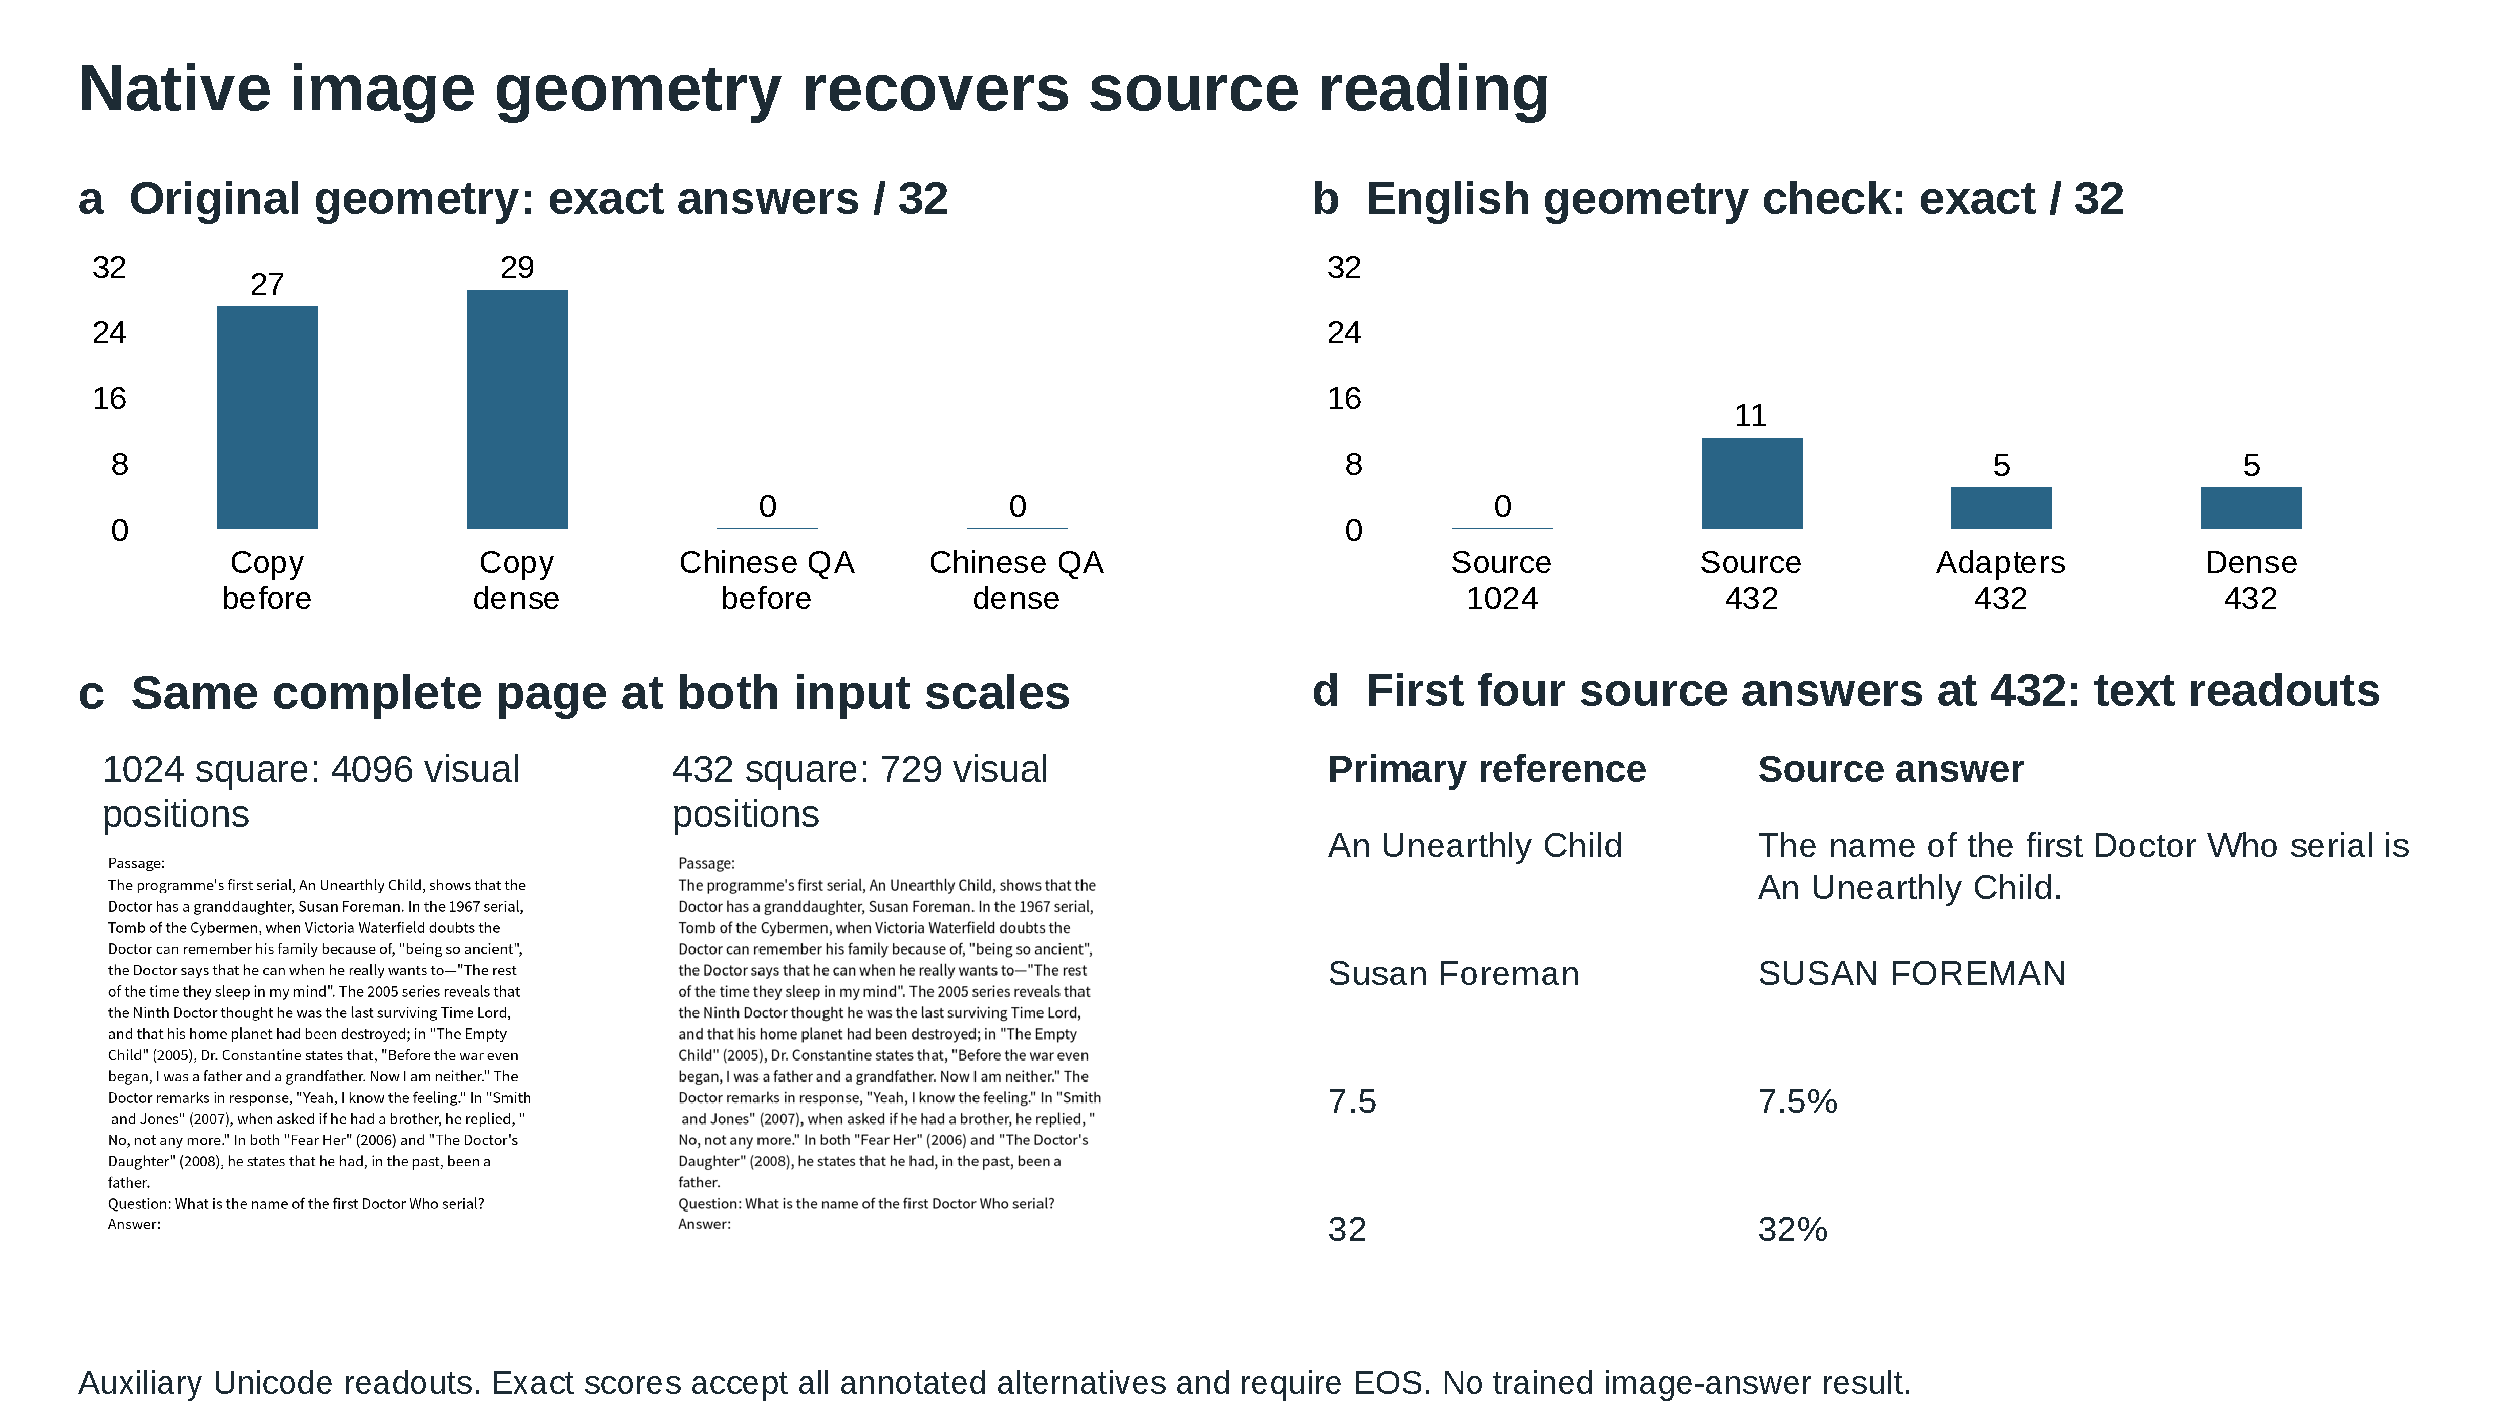
\includegraphics[width=\textwidth]{figures/Figure_S19_reader_geometry.pdf}\captionof{figure}{\textbf{Native image geometry recovers
source reading, while learned adapters remain weaker.} \textbf{a}, Complete
requested copying and Chinese QA at the original geometry before and after
the dense curriculum. \textbf{b}, Exact stopped English answers on the same
32 questions for frozen-source 1024, frozen-source 432 and the two completed
adapter states at 432. \textbf{c}, Complete first English page at both input
scales, shown at matched display size; full original canvases and PNG bytes
are embedded without cropping. This comparison documents the geometric
intervention rather than two independent samples. \textbf{d}, The first four
native-source text answers and their primary references, retained in fixed
order. Exact assessment accepts any annotated alternative and requires EOS;
extra wording and capitalization remain significant. These are auxiliary
text readouts, not answer images written by the learner. All 320 model calls
and failed answers remain available.}\label{fig:s19-reader-geometry}\end{minipage}

\clearpage
\section*{\DIFadd{Supplementary Note 43: state alignment and dependence on the canvas}}
\DIFadd{The frozen source's native-resolution English result in Note 42 does not
transfer to Chinese. On the fixed 32 Chinese questions, the source gives
0/32 exact stopped answers from either the original 1024-square image or its
432-square whole-image resize, versus 16/32 from the original visible text.
The latter is a privileged source-language control. Independent full-page
recognition of sampled codec reconstructions gives character errors 0.086875
at 1024 and 0.705221 at 432; these are readability observations, not proofs
of latent information loss. Native-scale semantic windows retain resolution
but give 0/32 Chinese and 2/32 English QA; pooling them to the native prefix
gives 0/32 in both languages. Neither frozen replacement qualifies reading.
}

\paragraph{\DIFadd{A source-preserving learned correction.}}
\DIFadd{For a complete image $X$, let $C(X)$ be the native 729-position visual feature
sequence from its whole-image 432-square resize. Let $F_A(X)$ encode the
original 1024-square image using nine overlapping native semantic windows,
with learned visual/fusion adapters $A$, then pool the fused 64-by-64 field
to 27 by 27. Both sequences have width 1,536. The corrected features are
}\[
 Z(X)=C(X)+G\bigl(F_A(X)-C(X)\bigr),\qquad G_0=0.
\]
\DIFadd{The bias-free full-rank $G$ has 2,359,296 parameters; 158 gated rank-16
visual/fusion adapters add 8,489,984. All original weights, the coarse
frontend, language body/head and image generator remain frozen. At zero
correction the complete native source prefix is exact. Pooling is lossy;
retaining all input pixels before pooling is not a lossless-context claim.
}

\DIFadd{The same frozen language body supplies offline original-text targets before
any correct answer history. For its final assistant-role state at layers
$\mathcal L=\{4,8,12,16,20,24,28\}$, define
}\[
 N(h)=\frac{h}{\sqrt{1536^{-1}\sum_d h_d^2+10^{-6}}},\qquad
 \mathcal L_{\rm state}=\frac{1}{7\cdot1536}
 \sum_{\ell\in\mathcal L}\|N(s_\ell)-N(t_\ell)\|_2^2.
\]
\DIFadd{Optimization minimizes answer cross entropy plus $\mathcal L_{\rm state}$,
with unit coefficients. Correct preceding answer history enters only the
cross-entropy term. The native mask blocks every future answer position
from the pre-answer states. The temporary FP32 causal check has normalized
maximum error $7.6294\times10^{-6}$, below $2\times10^{-5}$.
}

\DIFadd{All 640 training records appear four times: 128 copies, 256 Chinese questions
and 256 English questions from 128 paragraphs in 32 articles excluding all
sixteen English assessment articles. Preparation rejects only missing font
coverage or complete-page overflow, without teacher-outcome selection.
AdamW uses $(0.9,0.95)$, decay 0.01, norm clipping at one, 64-update warm-up
to $2\times10^{-5}$ and cosine decay to $2\times10^{-6}$. There is no
validation checkpoint selection. All 2,560 observations and finite gradients
are retained. The invocation takes 3,112.084\,s at 6.370\,GiB peak allocated
VRAM, excluding loading and the 238.713\,s offline cache. The complete adapted
model has 2,841,626,336 parameters plus the 126,892,531-parameter codec and
external pretraining; 10,849,280 trainable parameters do not define the full
model size.
}

\begin{center}\small
\begin{tabular}{lrr}
\toprule
\DIFadd{Fixed primary assessment }& \DIFadd{Native source }& \DIFadd{Learned correction}\\
\midrule
\DIFadd{English copying }& \DIFadd{7/16 }& \DIFadd{16/16}\\
\DIFadd{Chinese copying }& \DIFadd{0/16 }& \DIFadd{0/16}\\
\DIFadd{English QA }& \DIFadd{11/32 }& \DIFadd{16/32}\\
\DIFadd{Both English questions correct }& \DIFadd{3/16 }& \DIFadd{4/16}\\
\DIFadd{Chinese QA }& \DIFadd{0/32 }& \DIFadd{0/32}\\
\DIFadd{Both Chinese questions correct }& \DIFadd{0/16 }& \DIFadd{0/16}\\
\bottomrule
\end{tabular}
\end{center}
\DIFadd{English gains six correct answers and loses one on the same small, repeatedly
inspected cohort. Fifteen of sixteen correct learned answers become incorrect
without the passage; one remains correct without it. Chinese remains
unreliable: eleven of sixteen pairs give identical responses to different
questions. The first two references, \emph{India--West Pacific region} and
\emph{India Pondicherry}, both receive the shorter Chinese answer \emph{India}.
All normal Chinese responses stop, but stopping and related fragments are
not correctness. Four of the six declared reader requirements fail.
}

\DIFadd{The original preflight replays four native-source readouts, but compares the
corrected prefix/mask on only one training probe. The additional complete
four-case corrected-path check is performed after optimization, before final
scoring: four prefixes/masks and eight readouts match exactly. This timing
deviation is retained. The controller reuses the completed optimizer and
160 after-readouts; neither is restarted. No transcript, teacher state,
correct history or recognition output conditions autonomous assessment.
}

\paragraph{\DIFadd{Seen-prompt fit.}}
\DIFadd{A separate prospective diagnosis selects the first eight training records
per task and language before the primary after-readouts. All 96 calls
(source image, learner image and original-text source) stop. The learner
copies 8/8 English but 0/8 Chinese strings; all eight Chinese failures change
characters, including the first fixed case in Fig.~S20. Seen English QA
is 6/8 against original annotation alternatives, or 5/8 against its particular
cross-entropy target; strict Chinese QA is 0/8. The original-text control has
three exact Chinese copies, four further strings intact inside quotes and
one translated string. Several QA responses differ in language, surrounding
text or date formatting, while others give wrong quantities. Its strict 1/8
Chinese QA count is not a count of every semantically related answer.
No criteria are changed after inspection. The observed copying errors
establish a fit obstruction in this recipe, without identifying its unique
architectural or optimization cause. These are seen data, not generalization.
}

\paragraph{\DIFadd{A separate attention-only intervention.}}
\DIFadd{Starting instead from the dense checkpoint of Note 42, a second learner
freezes the complete calibrated visual frontend and trains fresh rank-16
residuals only in the 112 native q/k/v/o projections. Copying retains its
original strips and QA its complete square pages; no pooling or image resize
is introduced. All 640 bilingual records appear four times. The 4,358,144
new parameters receive answer cross entropy, with AdamW, 64-update warm-up
to $5\times10^{-5}$ and cosine decay to $5\times10^{-6}$. There is no
text-state teacher or validation selection. The complete adapted model has
2,843,625,184 parameters plus the same codec and external pretraining.
The 2,560-update invocation takes 1,667.861\,s at 6.345\,GiB peak allocated
memory, excluding loading and its 262.431\,s prefix cache. The real
three-update preflight preserves disabled-source logits exactly, changes
all 112 zero output matrices and gives finite nonzero gradients in all
224 residual tensors. Four disabled/zero source pairs replay exactly;
the normalized FP32 causal check has zero error. Nevertheless, the complete
160-call assessment retains 29/32 copies (Chinese 13/16, English 16/16)
but gives 0/32 QA in both languages, with no both-correct pairs. The first
English title and person questions both receive the unrelated year 1961.
All six reader requirements fail. These costs and outcomes belong to this
separate attention learner, not to the coarse/fine correction above. Its
complete export is }\path{references/evidence/native_reader_attention_result/}\DIFadd{.
}

\paragraph{\DIFadd{A controlled canvas failure.}}
\DIFadd{The 13/16 Chinese copying result in Note 42 uses 1024-by-256 strips, whereas
the correction study above uses complete 1024-square copying inputs. The
cross-model difference therefore cannot be attributed to pooling alone.
An independent 480-call control fixes the earlier dense checkpoint, its
seeds, generic instruction and all ink. All 160 original-layout decision
sequences replay exactly before altered layouts are evaluated. For every
copying request, white bottom padding gives the original square exactly:
}\[
 X_{\rm square}=\operatorname{pad}_{\rm white}(X_{\rm strip}).
\]
\DIFadd{The visual field changes from 1,024 to 4,096 positions. Exact copying falls
from 29/32 to 7/32: Chinese 13/16 to 0/16 and English 16/16 to 7/16.
No request character is resized, removed or moved. Ten padded copies fail
to stop within the 96-decision cap. A separate tight crop retains all pixels
unequal to white, adds a 16-pixel margin and rounds outward to multiples
of 16. It uses no recognition, transcript, font metric, answer or semantic
role. Replacing its white exterior reconstructs every source exactly, but
copying is 0/32. Fewer visual positions, 161--304 for these copies, do not
guarantee correct reading.
}

\DIFadd{Natural QA remains 0/32 in both languages in all three arms. The legacy and
square QA inputs are identical. Tight cropping changes their visual features,
positions and context lengths despite preserving the full visible request.
Pixel-level invertibility does not imply invariance of the learned mapping
$R(E(X))$. This control demonstrates geometric brittleness, not the unique
mechanism of failure. The three 160-call arms take 86.856, 120.337 and
64.060\,s excluding loading, with peaks 11.161, 11.161 and 10.506\,GiB.
Faster incorrect inference is not efficiency at matched useful quality.
}

\paragraph{\DIFadd{Separating source features from context layout.}}
\DIFadd{A prospectively fixed 128-call intervention uses the same frozen dense
checkpoint and all 32 copying requests. Let $S$ be the 1,024 strip features
and $Q$ the 4,096 square features; $Q_{\rm top}$ denotes its first 1,024
positions, covering the same upper 256 pixels. All request ink lies inside
that strip. Before any hybrid call, all 64 original strip and square
decision sequences replay exactly. Every pair has bit-identical nonvisual
headers and suffixes. The two hybrids use the native short or long mask,
respectively, without changing model parameters, instructions or readout.
}

\begin{center}\small
\begin{tabular}{lrrr}
\toprule
\DIFadd{Visual features }& \DIFadd{Prefix length }& \DIFadd{Chinese copies }& \DIFadd{English copies}\\
\midrule
\DIFadd{$S$ }& \DIFadd{1,063 }& \DIFadd{13/16 }& \DIFadd{16/16}\\
\DIFadd{$Q$ }& \DIFadd{4,135 }& \DIFadd{0/16 }& \DIFadd{7/16}\\
\DIFadd{$Q_{\rm top}$ }& \DIFadd{1,063 }& \DIFadd{0/16 }& \DIFadd{6/16}\\
\DIFadd{$[S;Q_{\rm tail}]$ }& \DIFadd{4,135 }& \DIFadd{2/16 }& \DIFadd{16/16}\\
\bottomrule
\end{tabular}
\end{center}
\DIFadd{Short context alone does not restore copying from the square's features.
Substituting strip features into the long context restores English copying,
but Chinese remains substantially below the strip source. These hybrid
prefixes need not encode real images. Nominally blank-region features can
contain global information; context changes also move the suffix and change
positions and available keys. Thus the comparison narrows the representation
failure without isolating a unique internal cause. All 128 raw responses
are retained. The invocation takes 68.220\,s after loading at 11.161\,GiB
peak allocated memory; the complete frozen model has 2,839,267,040 parameters
plus the same codec and external pretraining. There are no optimizer updates,
natural-QA measurements or image answers in this intervention.
}

\DIFadd{The full exports preserve all raw responses, input rasters, original
alternatives, seeds, executed-code hashes and reconstruction checks:
}\begin{quote}\footnotesize
\path{references/evidence/native_state_alignment_result/}\\
\path{references/evidence/native_state_fit_result/}\\
\path{references/evidence/native_canvas_control_result/}\\
\path{references/evidence/native_canvas_factorization_result/}
\end{quote}
\DIFadd{The state study's public per-update journal is compact; its full per-parameter
gradient journal remains local with SHA256. The canvas export binds all 480
source PNGs. CMRC 2018 and SQuAD 1.1 retain CC-BY-SA-4.0 attribution; the
Show-o2 source/model are NUS Show Lab, Apache-2.0. These auxiliary Unicode
head results do not demonstrate continuous image answers. The failed Chinese
requirements do not admit scaling or a writing-stage qualification.
}

\clearpage
\plate{Figure_S20_state_alignment}{\textbf{Limited English transfer and a
controlled failure of geometric invariance.} \textbf{a}, Source-preserving
coarse/fine correction; orange layers learn, while the native language
body and temporary text head remain frozen. Offline text-state targets
and correct answer history are training supervision only. \textbf{b}, Exact
stopped English/Chinese QA on the same 32 questions before and after the
2,560-update correction. Copying counts are shown separately. \textbf{c},
The separate earlier dense checkpoint under three whole-request layouts;
all weights and sampling seeds are fixed, and every ink pixel is preserved.
This is not a cross-model comparison. \textbf{d}, The first fixed seen
Chinese copying request and raw auxiliary text response. Only white
exterior is omitted for display; the learner receives the complete square.
The visible request pixels are retained exactly. The separately labelled
attention-only result in the footer belongs to a different learner, which
retains copying but fails QA. The editable text is a
Unicode-head readout, not an answer image generated by the learner.
All failures remain in the complete exports.}{fig:s20-state-alignment}


\clearpage
\DIFaddend \section*{Reproduction}
From the repository root, use the following entry points. GPU stages use
physical GPU 0; preparation and independent pixel checks run on CPU.
\begin{quote}\small\ttfamily
CUDA\_VISIBLE\_DEVICES=0 PYTHONPATH=. python\\
scripts/train\_causal\_visual\_block\_diffusion\_v53.py --device cuda:0
\end{quote}
\begin{quote}\small\ttfamily
CUDA\_VISIBLE\_DEVICES=0 PYTHONPATH=. python\\
scripts/eval\_causal\_visual\_block\_diffusion\_v53.py --device cuda:0
\end{quote}
Completed output directories are protected against accidental replacement.
For the exact density, with the same GPU selection, use
\begin{quote}\small\ttfamily
scripts/train\_exact\_raster\_density\_v54.py\\
scripts/eval\_exact\_raster\_density\_v54.py
\end{quote}
Independent image inference and export use
\begin{quote}\small\ttfamily
scripts/infer\_exact\_raster\_density\_v54.py.
\end{quote}
For the matched continuation, run the following with \texttt{--arm frozen}
and then \texttt{--arm joint}, completing both before the evaluator:
\begin{quote}\small\ttfamily
scripts/train\_joint\_exact\_raster\_v55.py\\
scripts/eval\_joint\_exact\_raster\_v55.py
\end{quote}
The independent runtime uses
\texttt{scripts/infer\_joint\_exact\_raster\_v55.py}.
The form diagnostic and locked pixel decoder audit use
\begin{quote}\small\ttfamily
scripts/diagnose\_raster\_form\_validity.py\\
scripts/eval\_raster\_beam\_v56.py.
\end{quote}
Independent pixel-beam inference uses
\texttt{scripts/infer\_raster\_beam.py}.
For grounded visual reading, complete both training arms before auditing:
\begin{quote}\small\ttfamily
scripts/train\_visual\_copy\_language\_v57.py --arm copy\\
scripts/train\_visual\_copy\_language\_v57.py --arm no\_copy\\
scripts/eval\_visual\_copy\_language\_v57.py.
\end{quote}
Native answers and self-contained export use
\begin{quote}\small\ttfamily
scripts/infer\_visual\_copy\_language.py.
\end{quote}
For complete image blocks, train both arms before the audit:
\begin{quote}\small\ttfamily
scripts/train\_visual\_answer\_blocks\_v58.py\\
scripts/eval\_visual\_answer\_blocks\_v58.py.
\end{quote}
Native inference uses
\begin{quote}\small\ttfamily
scripts/infer\_visual\_answer\_blocks.py.
\end{quote}
Frozen-feature preparation, matched readout training and audit use the
\texttt{cache\_frozen\_visual\_features\_v59},
\texttt{train\_frozen\_visual\_readout\_v59} and
\texttt{eval\_frozen\_visual\_readout\_v59} scripts.
The matched input-order experiment runs both orders before auditing:
\begin{quote}\small\ttfamily
scripts/train\_question\_first\_reading\_v60.py\\
--order context\\
--order question\\
scripts/eval\_question\_first\_reading\_v60.py.
\end{quote}
Native pixel preparation, full adaptation and locked audit use the existing
Python 3.12 MIXAR runtime, with \texttt{CUDA\_VISIBLE\_DEVICES=0}:
\begin{quote}\small\ttfamily
scripts/prepare\_native\_pixel\_qa\_v61.py\\
scripts/train\_native\_pixel\_instruction\_v61.py\\
scripts/verify\_native\_pixel\_export\_v61.py\\
scripts/eval\_native\_pixel\_instruction\_v61.py.
\end{quote}
Independent image inference uses
\texttt{scripts/infer\_native\_pixel\_language.py}.
The matched whole-image experiment uses the persistent sequential coordinator
\begin{quote}\small\ttfamily
scripts/run\_correlated\_native\_v62.py.
\end{quote}
It verifies both complete training reports, standalone offline replays and
the locked audit in that order. Independent image inference uses
\texttt{scripts/infer\_correlated\_native\_language.py};
the exported bundle's \texttt{run.py} does not need the repository or the
original foundation checkpoint. The optional, separately calibrated vision
diagnostic is \texttt{scripts/audit\_correlated\_native\_transcripts\_v62.py}.
That reader stays outside the actor and changes no primary gate.
The complete assignment comparison uses
\path{scripts/run_question_assignment_v63.py}; its independent raw-score
verification is \path{scripts/verify_question_assignment_result_v63.py}.
The separate successor preflight is \path{scripts/check_grounded_image_actor.py},
and its helper-only source check is \path{scripts/check_inherited_context.py}.
The writing-only curriculum is specified in
\path{references/grounded_writer_learning_protocol.md}; it is not an
additional completed language result.

The matched writer diagnosis and broader direct stage use
\path{scripts/diagnose_grounded_writer_v65.py} and
\path{scripts/train_direct_grounded_writer_v66.py}; their independent
verifiers retain the failed fidelity decisions. The separate output-codec
audit is \path{scripts/audit_codec_output_v67.py}, with native replay in
\path{scripts/verify_codec_output_v67.py}. Complete separate-space actor
execution is checked by \path{scripts/check_codec_visual_language_actor.py}.
The fixed instruction-learning protocol is
\path{references/codec_language_learning_v68_protocol.md}; its training entry
point is \path{scripts/train_codec_language_v68.py}. Prepared prompt images
and blank controls use \path{scripts/prepare_codec_language_audit_v68.py}.
The evaluator \path{scripts/eval_codec_language_v68.py} accepts only the final
10,000-update state and has a separate CPU data/metric preflight. Its
independent raw-stream verifier is \path{scripts/verify_codec_language_v68.py}.
These entry points produce the completed, failed autonomous result in
Supplementary Note 27. The source-bound integrity and output-verification
receipts are retained in \path{references/evidence/}.

The frozen-actor diagnostic is
\path{scripts/diagnose_codec_language_v68.py}. In the compatible native
PyTorch environment, use \texttt{--prepare-only} with CUDA hidden, then run
the same command on physical GPU 0 with the deterministic cuBLAS configuration,
and finally use \texttt{--verify-only} with CUDA hidden. Supply the same fresh
\texttt{--out} directory for those phases; completed measurements are never
overwritten. The source-frozen selection, assisted-history scope and
measurement checks are defined in
\path{references/codec_language_v68_diagnosis_protocol.md}.

\DIFdelbegin %DIFDELCMD < \begin{thebibliography}{18}
%DIFDELCMD < %%%
\DIFdelend \DIFaddbegin \DIFadd{The completed native-context run in Note 37 uses the compatible existing
Python 3.12 environment and authenticated local image, code and weight caches.
GPU phases require \texttt{CUDA\_VISIBLE\_DEVICES=0} and
\texttt{CUBLAS\_WORKSPACE\_CONFIG=:4096:8}. Its training and complete audit
entry points are }\path{scripts/train_native_chinese_v80.py} \DIFadd{and
}\path{scripts/audit_native_chinese_v80.py}\DIFadd{; the latter's \texttt{--verify}
phase runs with CUDA hidden. The fixed training-cohort controls use
}\path{scripts/probe_native_corpus_fit_v80.py}\DIFadd{, with separate
\texttt{--stage prepare}, \texttt{--stage evaluate} and
\texttt{--stage verify} invocations, and the same explicit source run and
fresh output directory. Preparation and verification run with CUDA hidden;
evaluation uses the GPU environment above. Exact arguments, source identities
and retained failure handling are specified in
}\path{references/native_chinese_v80_protocol.md}\DIFadd{,
}\path{references/native_corpus_fit_v80_protocol.md} \DIFadd{and
}\path{docs/native-image-continuation.md}\DIFadd{.
}

\DIFadd{The matched readout experiment in Note 38 uses
}\path{scripts/train_adaptive_readout_v81.py} \DIFadd{with separate preflight and
training stages. Preserve its failed original evaluation and partial output.
The completed checkpoints are evaluated without optimization using
}\path{scripts/evaluate_trained_readout_v81.py}\DIFadd{, first with
\texttt{--stage evaluate} in the deterministic GPU0 environment above, then
\texttt{--stage verify} with CUDA explicitly hidden. Export all verified
images and scores with }\path{scripts/export_readout_v81_result.py}\DIFadd{.
The source-bound execution and numerical criteria are in
}\path{references/adaptive_readout_v81_protocol.md}\DIFadd{,
}\path{references/adaptive_readout_v81r2_protocol.md} \DIFadd{and
}\path{references/adaptive_readout_v81_evaluation_protocol.md}\DIFadd{.
}

\DIFadd{The matched decoder-sensitive comparison in Note 39 uses
}\path{scripts/train_decoder_metric_v82.py} \DIFadd{with separate preflight, training
and CPU verification stages, under
}\path{references/decoder_metric_v82_protocol.md} \DIFadd{and
}\path{references/decoder_metric_v82r2_protocol.md}\DIFadd{. Preserve the first failed
execution and interruption records. Export the verified complete cohort with
}\path{scripts/export_decoder_metric_v82_result.py}\DIFadd{. Independently reproduce
the spatial failure diagnosis from the public PNGs using
}\path{scripts/diagnose_writing_failures.py}\DIFadd{. Standalone execution uses
}\path{scripts/infer_decoder_metric_v82.py}\DIFadd{; the fixed one-case restoration
check is }\path{scripts/check_metric_runtime_replay_v82.py}\DIFadd{.
}

\DIFadd{The paired-image experiment in Note 40 uses
}\path{scripts/prepare_paired_image_condition.py} \DIFadd{for the standalone offline
constant, }\path{scripts/train_paired_image_language.py} \DIFadd{for preparation,
caching, preflight, optimization and single-image inference, and
}\path{scripts/infer_paired_image_cohort.py} \DIFadd{for a fresh input-only cohort.
The fixed preprocessing is }\path{scripts/trim_paired_input_padding.py}\DIFadd{;
separate CPU recognition is }\path{scripts/score_paired_writing.py}\DIFadd{.
Authenticate the complete export with
}\path{scripts/export_paired_padding_result.py}\DIFadd{. Protocols and full command
examples are in }\path{references/paired_image_learning_protocol.md}\DIFadd{,
}\path{references/paired_padding_protocol.md}\DIFadd{,
}\path{references/paired_padding_full_cohort_protocol.md} \DIFadd{and
}\path{docs/paired-image-learning.md}\DIFadd{.
}

\DIFadd{The native source and visual-access observation in Note 41 use
}\path{scripts/acquire_native_unified_source.py}\DIFadd{,
}\path{scripts/probe_native_unified_source.py} \DIFadd{and
}\path{scripts/train_native_visual_access.py}\DIFadd{. Complete held-out preparation
and matched question interventions use
}\path{scripts/prepare_native_visual_access_validation.py} \DIFadd{and
}\path{scripts/probe_native_visual_access_controls.py}\DIFadd{. CPU export uses
}\path{scripts/score_native_visual_access.py}\DIFadd{. Fixed protocols, the isolated
runtime, exact commands and the remaining image-writing requirement are in
}\path{docs/native-visual-access.md} \DIFadd{and
}\path{references/native_visual_access_assessment_protocol.md}\DIFadd{.
}

\DIFadd{The full-page curriculum in Note 42 uses
}\path{scripts/prepare_native_visual_alignment.py}\DIFadd{,
}\path{scripts/train_native_visual_alignment.py} \DIFadd{and
}\path{scripts/score_native_visual_alignment.py}\DIFadd{. Prospective English pages and
source readability checks use }\path{scripts/prepare_native_english_transfer.py}
\DIFadd{and }\path{scripts/score_native_english_transfer.py}\DIFadd{. The geometry intervention
uses }\path{scripts/check_native_reader_geometry.py}\DIFadd{,
}\path{scripts/probe_native_unadapted_reader.py} \DIFadd{and
}\path{scripts/score_native_reader_geometry.py}\DIFadd{. All inference indexes exclude
answer strings. Exact commands, fresh output paths and sequential GPU stages
are specified in }\path{docs/native-visual-alignment.md}\DIFadd{,
}\path{docs/native-english-transfer.md} \DIFadd{and
}\path{references/native_reader_geometry_result.md}\DIFadd{.
}

\begin{thebibliography}{21}
\DIFaddend \small
\interlinepenalty=5000
\bibitem{pixar} Tai, Y., Liao, X., Suglia, A. \& Vergari, A. PIXAR: Auto-Regressive Language Modeling in Pixel Space. \emph{arXiv} 2401.03321 (2024). \url{https://arxiv.org/abs/2401.03321}.
\bibitem{mar} Li, T., Tian, Y., Li, H., Deng, M. \& He, K. Autoregressive Image Generation without Vector Quantization. \emph{Advances in Neural Information Processing Systems} (2024). \url{https://arxiv.org/abs/2406.11838}.
\bibitem{forcing} Chen, B. et al. Diffusion Forcing: Next-token Prediction Meets Full-Sequence Diffusion. \emph{arXiv} 2407.01392 (2024). \url{https://arxiv.org/abs/2407.01392}.
\bibitem{guidance} Dhariwal, P. \& Nichol, A. Diffusion Models Beat GANs on Image Synthesis. \emph{Advances in Neural Information Processing Systems} (2021). \url{https://arxiv.org/abs/2105.05233}.
\bibitem{repa} Yu, S. et al. Representation Alignment for Generation: Training Diffusion Transformers Is Easier Than You Think. \emph{International Conference on Learning Representations} (2025). \url{https://arxiv.org/abs/2410.06940}.
\bibitem{pixelrnn} van den Oord, A., Kalchbrenner, N. \& Kavukcuoglu, K. Pixel Recurrent Neural Networks. \emph{Proceedings of the 33rd International Conference on Machine Learning} \textbf{48}, 1747--1756 (2016). \url{https://proceedings.mlr.press/v48/oord16.html}.
\bibitem{pixelcnn} van den Oord, A. et al. Conditional Image Generation with PixelCNN Decoders. \emph{arXiv} 1606.05328 (2016). \url{https://arxiv.org/abs/1606.05328}.
\bibitem{made} Germain, M., Gregor, K., Murray, I. \& Larochelle, H. MADE: Masked Autoencoder for Distribution Estimation. \emph{Proceedings of the 32nd International Conference on Machine Learning} \textbf{37}, 881--889 (2015). \url{https://arxiv.org/abs/1502.03509}.
\bibitem{mixar} Hu, C., Tai, Y., Vergari, A., Keller, F. \& Suglia, A. MIXAR: Scaling Autoregressive Pixel-based Language Models to Multiple Languages and Scripts. \emph{arXiv} 2604.11575v2 (2026). \url{https://arxiv.org/abs/2604.11575v2}.
\bibitem{degeneration} Holtzman, A., Buys, J., Du, L., Forbes, M. \& Choi, Y. The Curious Case of Neural Text Degeneration. \emph{International Conference on Learning Representations} (2020). \url{https://arxiv.org/abs/1904.09751}.
\bibitem{pointer} See, A., Liu, P. J. \& Manning, C. D. Get To The Point: Summarization with Pointer-Generator Networks. \emph{Proceedings of ACL}, 1073--1083 (2017). \url{https://aclanthology.org/P17-1099/}.
\bibitem{cmrc} Cui, Y. et al. A Span-Extraction Dataset for Chinese Machine Reading Comprehension. \emph{Proceedings of EMNLP-IJCNLP}, 5883--5889 (2019). \url{https://aclanthology.org/D19-1600/}.
\bibitem{mgflow} Zhang, C. et al. Unifying Distributional Training for One-Step Visual Generation. \emph{arXiv} 2609.35763v4 (2026). \url{https://arxiv.org/abs/2609.35763v4}.
\bibitem{semot} Van Assel, H., De Brouwer, E., Saremi, S., Scalia, G. \& Regev, A. Generate in Reconstruction Space, Match in Semantic Space: Transport Geometry for One-Step Generation. \emph{arXiv} 2606.00514v2 (2026). \url{https://arxiv.org/abs/2606.00514v2}.
\bibitem{multimodalflow} Tao, H. et al. Multimodal Flow: Unified Flow Modeling of Language and Vision in Embedding Spaces. \emph{arXiv} 2609.40362v1 (2026). \url{https://arxiv.org/abs/2609.40362v1}.
\bibitem{ocg} Huang, L. \& Wu, X. OCG: Optical Character Grounded Visual Reasoning with Flow Matching. \href{https://www.alphaxiv.org/abs/2608.ocg-optical-character-grounded-reasoning}{Author manuscript} (2026). Peer-review status unverified.
\bibitem{qwen3vl} Bai, S. et al. Qwen3-VL Technical Report. \emph{arXiv} 2511.21631v2 (2025). \url{https://arxiv.org/abs/2511.21631v2}.
\bibitem{dolly} Databricks. Databricks Dolly 15k instruction dataset (2023). \url{https://huggingface.co/datasets/databricks/databricks-dolly-15k}\DIFaddbegin \DIFadd{.
}\bibitem{jit} \DIFadd{Li, T. \& He, K. Back to Basics: Let Denoising Generative Models Denoise. \emph{arXiv} 2511.13720v1 (2025). }\url{https://arxiv.org/abs/2511.13720v1}\DIFadd{.
}\bibitem{showo2} \DIFadd{Xie, J., Yang, Z. \& Shou, M. Z. Show-o2: Improved Native Unified Multimodal Models. \emph{arXiv} 2506.15564v3 (2025). }\url{https://arxiv.org/abs/2506.15564v3}\DIFadd{.
}\bibitem{squad} \DIFadd{Rajpurkar, P., Zhang, J., Lopyrev, K. \& Liang, P. SQuAD: 100,000+ Questions for Machine Comprehension of Text. \emph{Proceedings of EMNLP}, 2383--2392 (2016). }\url{https://aclanthology.org/D16-1264/}\DIFaddend .
\end{thebibliography}

\end{document}
